%%%%%%%%%%%%%%%%%%%%%%%%%%%%%%%%%%%%%%%%%
% Masters/Doctoral Thesis 
% LaTeX Template
% Version 2.3 (25/3/16)
%
% This template has been downloaded from:
% http://www.LaTeXTemplates.com
%
% Version 2.x major modifications by:
% Vel (vel@latextemplates.com)
%
% This template is based on a template by:
% Steve Gunn (http://users.ecs.soton.ac.uk/srg/softwaretools/document/templates/)
% Sunil Patel (http://www.sunilpatel.co.uk/thesis-template/)
%
% Template license:
% CC BY-NC-SA 3.0 (http://creativecommons.org/licenses/by-nc-sa/3.0/)
%
%%%%%%%%%%%%%%%%%%%%%%%%%%%%%%%%%%%%%%%%%

%----------------------------------------------------------------------------------------
%	PACKAGES AND OTHER DOCUMENT CONFIGURATIONS
%----------------------------------------------------------------------------------------

\documentclass[
12pt, % The default document font size, options: 10pt, 11pt, 12pt
%oneside, % Two side (alternating margins) for binding by default, uncomment to switch to one side
%chapterinoneline,% Have the chapter title next to the number in one single line
%nfrench
ngerman,
english, % ngerman for German
%singlespacing, % Single line spacing, alternatives: onehalfspacing or doublespacing
onehalfspacing,
hidelinks,
%draft, % Uncomment to enable draft mode (no pictures, no links, overfull hboxes indicated)
%nolistspacing, % If the document is onehalfspacing or doublespacing, uncomment this to set spacing in lists to single
%liststotoc, % Uncomment to add the list of figures/tables/etc to the table of contents
toctotoc, % Uncomment to add the main table of contents to the table of contents
%parskip, % Uncomment to add space between paragraphs
%nohyperref, % Uncomment to not load the hyperref package
headsepline, % Uncomment to get a line under the header
%openany\usepackage{float}
]{MastersDoctoralThesis} % The class file specifying the document structure

\usepackage[utf8]{inputenc} % Required for inputting international characters
\usepackage[euler]{textgreek}
\usepackage{graphicx}
\usepackage[T1]{fontenc} % Output font encoding for international characters
\usepackage{microtype}
%\usepackage{fontspec}
%\usepackage{palatino} % Use the Palatino font by default
\usepackage[nottoc,notlot,notlof]{tocbibind}

%\bibliographystyle{IEEEtran}
%\bibliography{/Users/kaksonenlab/Desktop/dm/thesis_git/cloned/parts/references}


%\usepackage{nimbusserif} % Use the Palatino font by default
\usepackage{gfsdidot}
%\setmainfont{Charis SIL}

\usepackage[backend=bibtex,style=authoryear,maxcitenames=2,maxbibnames=9,natbib=true]{biblatex} % Use the bibtex backend with the authoryear citation style (which resembles APA)
\usepackage{breakcites}
%\addbibresource{refs.bib} % The filename of the bibliography


\usepackage[autostyle=true]{csquotes} % Required to generate language-dependent quotes in the bibliography
\usepackage{hyperref}
\usepackage[margin=10pt,font=small,textfont=footnotesize, labelfont=bf, justification=justified,labelsep=endash]{caption}
%\usepackage{caption}
%\captionsetup{width=\linewidth}
%	COunter for numbering
\setcounter{secnumdepth}{3}

\usepackage{textcomp} % for degree symbol \textdegree
\usepackage{float}
\usepackage{tabularx,tabu,longtable,etoolbox}

%\usepackage{morefloats}
\usepackage{afterpage}
\usepackage{placeins}
\newcommand\blankpage{%
	\null
	\thispagestyle{empty}%
%	\addtocounter{page}{-1}%
	\newpage}
\usepackage{pdflscape}
\usepackage{rotating}
\usepackage{needspace}
\usepackage{titlesec, blindtext, color}
\definecolor{gray75}{gray}{0.75}
\newcommand{\hsp}{\hspace{20pt}}
\titleformat{\chapter}[hang]{\Huge\bfseries}{\thechapter\hsp\textcolor{gray75}{|}\hsp}{0pt}{\Huge\bfseries}

\usepackage[export]{adjustbox}
%----------------------------------------------------------------------------------------
%	MARGIN SETTINGS
%----------------------------------------------------------------------------------------

\geometry{
	paper=a4paper, % Change to letterpaper for US letter
	inner=2.5cm, % Inner margin
	outer=3cm, % Outer margin
	bindingoffset=2cm, % Binding offset
	top=1.5cm, % Top margin
	bottom=1.5cm, % Bottom margin
	%showframe,% show how the type block is set on the page
}

%----------------------------------------------------------------------------------------
%	THESIS INFORMATION
%----------------------------------------------------------------------------------------

%\thesistitle{Regulation of membrane scission in yeast endocytosis} % Your thesis title, this is used in the title and abstract, print it elsewhere with \ttitle
%\supervisor{Dr. Jonas \textsc{Ries}} % Your supervisor's name, this is used in the title page, print it elsewhere with \supname
%\examiner{} % Your examiner's name, this is not currently used anywhere in the template, print it elsewhere with \examname
%\degree{Dr. rer. nat.} % Your degree name, this is used in the title page and abstract, print it elsewhere with \degreename
%\author{Markus Mund} % Your name, this is used in the title page and abstract, print it elsewhere with \authorname
%\addresses{} % Your address, this is not currently used anywhere in the template, print it elsewhere with \addressname

%\subject{Biological Sciences} % Your subject area, this is not currently used anywhere in the template, print it elsewhere with \subjectname
%\keywords{Clathrin-mediated endocytosis, budding yeast, superresolution microscopy, single-molecule localization, high-throughput imaging, Actin nucleation} % Keywords for your thesis, this is not currently used anywhere in the template, print it elsewhere with \keywordnames
%\university{\href{https://www.uni-heidelberg.de}{Ruperto-Carola University of Heidelberg, Germany}} % Your university's name and URL, this is used in the title page and abstract, print it elsewhere with \univname
%\department{\href{http://department.university.com}{Department or School Name}} % Your department's name and URL, this is used in the title page and abstract, print it elsewhere with \deptname
%\group{\href{http://researchgroup.university.com}{Research Group Name}} % Your research group's name and URL, this is used in the title page, print it elsewhere with \groupname
%\faculty{\href{http://faculty.university.com}{Faculty Name}} % Your faculty's name and URL, this is used in the title page and abstract, print it elsewhere with \facname

%%\thesistitle{Regulation of membrane scission in yeast endocytosis} % Your thesis title, this is used in the title and abstract, print it elsewhere with \ttitle
%%\supervisor{Dr. Jonas \textsc{Ries}} % Your supervisor's name, this is used in the title page, print it elsewhere with \supname
%%\examiner{} % Your examiner's name, this is not currently used anywhere in the template, print it elsewhere with \examname
%%\degree{Dr. rer. nat.} % Your degree name, this is used in the title page and abstract, print it elsewhere with \degreename
%%\author{Deepikaa Menon} % Your name, this is used in the title page and abstract, print it elsewhere with \authorname
%%\addresses{} % Your address, this is not currently used anywhere in the template, print it elsewhere with \addressname

%%\subject{Biological Sciences} % Your subject area, this is not currently used anywhere in the template, print it elsewhere with \subjectname
%%\keywords{Clathrin-mediated endocytosis, budding yeast, superresolution microscopy, single-molecule localization, high-throughput imaging, Actin nucleation} % Keywords for your thesis, this is not currently used anywhere in the template, print it elsewhere with \keywordnames
%%\university{\href{https://www.uni-heidelberg.de}{Ruperto-Carola University of Heidelberg, Germany}} % Your university's name and URL, this is used in the title page and abstract, print it elsewhere with \univname
%%\department{\href{http://department.university.com}{Department or School Name}} % Your department's name and URL, this is used in the title page and abstract, print it elsewhere with \deptname
%%\group{\href{http://researchgroup.university.com}{Research Group Name}} % Your research group's name and URL, this is used in the title page, print it elsewhere with \groupname
%\faculty{\href{http://faculty.university.com}{Faculty Name}} % Your faculty's name and URL, this is used in the title 

%%%\hypersetup{pdftitle=\ttitle} % Set the PDF's title to your title
%%%\hypersetup{pdfauthor=\authorname} % Set the PDF's author to your name
%\hypersetup{pdfkeywords=\keywordnames} % Set the PDF's keywords to your keywords

\begin{document}

%\frontmatter % Use roman page numbering style (i, ii, iii, iv...) for the pre-content pages

\pagestyle{plain} % Default to the plain heading style until the thesis style is called for the body content

%----------------------------------------------------------------------------------------
%	TITLE PAGE
%----------------------------------------------------------------------------------------
%
\begin{titlepage}
%\begin{left}
%\vspace*{0.2\textheight}

%\noindent\large{UNIVERSIT\'E DE GEN\`EVE\hspace*{\fill} EMBL\\
\noindent\large{UNIVERSIT\'E DE GEN\`EVE\\
Section de chimie et biochimie\\
Department de biochimie\\}
Professeur Marko Kaksonen\\
\noindent\rule{13.6cm}{0.4pt}

\vspace{2cm}
\begin{center}
\LARGE\textbf{REGULATION OF MEMBRANE SCISSION IN YEAST ENDOCYTOSIS} \\
	\vspace{1.5cm}
\end{center}

\begin{center}	
	{TH\`ESE\\
	present\'ee \`a la Facult\'e des sciences de l'Universit\'e de Gen\`eve\\
	pour obtenir le grade de Docteur \`es sciences, mention biochemie\\}
%Oral examination: November 25\textsuperscript{th} 2016}

\vspace{1.5cm}
	par\\
	Deepikaa Menon\\
%	\vspace{1cm}
	de\\
	Chennai (India)\\
	\vspace{2cm}
	Th\`ese N\r{} xxxx\\
	\vspace{1cm}
	GEN\`EVE / HEIDELBERG\\
	photoshop EMBL\\	
	2018\\
	
	
\end{center}

%\end{center}
%\afterpage{\blankpage}
\end{titlepage}


%\begin{titlepage}
%	    \begin{center}
%	    	\vspace*{3cm}
%	    	\Huge\textbf{Superresolution imaging of clathrin-mediated endocytosis\\ in yeast}
%	    \end{center}
%	    \vspace*{\fill}
%	    \Large{
%	    	\begin{tabular}{l l}
%	    		Referees: & Prof. Dr. Marko Kaksonen \\
%	    		& Prof. Dr. Michael Knop \\
%	    	\end{tabular}}
%\afterpage{\blankpage} 
%\end{titlepage}


%
%{\scshape\LARGE \univname\par}\vspace{1.5cm} % University name
%\textsc{\Large Doctoral Thesis}\\[0.5cm] % Thesis type
%
%\HRule \\[0.4cm] % Horizontal line
%{\huge \bfseries \ttitle\par}\vspace{0.4cm} % Thesis title
%\HRule \\[1.5cm] % Horizontal line
% 
%\begin{minipage}[t]{0.4\textwidth}
%\begin{flushleft} \large
%\emph{Author:}\\
%\href{http://www.johnsmith.com}{\authorname} % Author name - remove the \href bracket to remove the link
%\end{flushleft}
%\end{minipage}
%\begin{minipage}[t]{0.4\textwidth}
%\begin{flushright} \large
%\emph{Supervisor:} \\
%\href{http://www.jamessmith.com}{\supname} % Supervisor name - remove the \href bracket to remove the link  
%\end{flushright}
%\end{minipage}\\[3cm]
% 
%\large \textit{A thesis submitted in fulfillment of the requirements\\ for the degree of \degreename}\\[0.3cm] % University requirement text
%\textit{in the}\\[0.4cm]
%\groupname\\\deptname\\[2cm] % Research group name and department name
% 
%{\large \today}\\[4cm] % Date
%%\includegraphics{Logo} % University/department logo - uncomment to place it
% 

%
%%----------------------------------------------------------------------------------------
%%	DECLARATION PAGE
%%----------------------------------------------------------------------------------------
%
%\begin{declaration}
%\addchaptertocentry{\authorshipname}
%
%\noindent I, \authorname, declare that this thesis titled, \enquote{\ttitle} and the work presented in it are my own. I confirm that:
%
%\begin{itemize} 
%\item This work was done wholly or mainly while in candidature for a research degree at this University.
%\item Where any part of this thesis has previously been submitted for a degree or any other qualification at this University or any other institution, this has been clearly stated.
%\item Where I have consulted the published work of others, this is always clearly attributed.
%\item Where I have quoted from the work of others, the source is always given. With the exception of such quotations, this thesis is entirely my own work.
%\item I have acknowledged all main sources of help.
%\item Where the thesis is based on work done by myself jointly with others, I have made clear exactly what was done by others and what I have contributed myself.\\
%\end{itemize}
% 
%\noindent Signed:\\
%\rule[0.5em]{25em}{0.5pt} % This prints a line for the signature
% 
%\noindent Date:\\
%\rule[0.5em]{25em}{0.5pt} % This prints a line to write the date
%\end{declaration}
%
%\cleardoublepage

%----------------------------------------------------------------------------------------
%	QUOTATION PAGE
%----------------------------------------------------------------------------------------
%\addtocounter{page}{2}%
%\vspace*{0.2\textheight}

%\noindent\enquote{\itshape Basic research is what I'm doing when I don't know what I'm doing.}\bigbreak

%\hfill Wernher von Braun

%\null\vfill

%\noindent{}Parts of the work described in this thesis have been published:

%\bigskip

%\noindent\textbf{Mund, M.}, Kaplan, C., \& Ries, J. (2014). Localization microscopy in yeast. Methods in Cell Biology, 123, 253–271.

%\bigskip

%\noindent{}Picco, A., \textbf{Mund, M.}, Ries, J., Nédélec, F., \& Kaksonen, M. (2015). Visualizing the functional %architecture of the endocytic machinery. eLife, 4, 1039.

%----------------------------------------------------------------------------------------
%	ABSTRACT PAGE
%----------------------------------------------------------------------------------------

\begin{abstract}
\addchaptertocentry{Abstract} % Add the abstract to the table of contents
\begin{center}{\huge{Abstract} \par}\end{center}
\bigskip



Endocytosis is an ancient pathway that regulates communication of the cell with its environment. During this process, the plasma membrane is deformed in a controlled sequence: a flat membrane forms an invagination that undergoes scission to produce a cargo-filled vesicle. Breaking the membrane invagination to form a vesicle is perhaps the most dramatic shape transition in this development. This has excited a large body of literature on the cause of membrane scission. Work on mammalian cells has converged on a scission mechanism based on membrane neck constriction by the GTPase dynamin. A clear understanding of what causes scission remains incomplete for the much simpler endocytic network in yeast cells. 

		\vspace{5mm}
In this thesis, I investigate the mechanism of membrane scission in  \textit{Saccharomyces cerevisiae} and the proteins involved by combining mutagenesis with live-cell imaging of fluorescently tagged proteins. 

		\vspace{5mm}
Endocytic sites are very stereotypic in yeast, recruiting about 50 proteins- most with mammalian homologues- in a highly specific sequence. These proteins can be assigned to separable modules based on their role in the endocytosis. Members of the coat module arrive when the membrane is still flat and form the template for invagination. Actin regulators arrive later and produce the forces required to pull up the membrane. Scission proteins arrive at the end of the timeline and regulate vesicle formation. 

		\vspace{5mm}
The yeast BAR domain complex Rvs is an important regulator of scission: in cells without Rvs, scission efficiency decreases by nearly 30\%. The 70\% of invaginations that undergo scission in the cells form smaller vesicles than usual. Rvs thus appears to regulate both timing and likelihood of scission, but it has not been clear how it does so, or how it gets recruited to membrane tubes in the first place. 

		\vspace{5mm}
I find that Rvs localization is timed by its BAR domain. The BAR domain senses a particular membrane shape, and Rvs is only recruited to endocytic sites once this shape is acquired. Surprisingly, localization efficiency and localization itself is affected by a second domain of Rvs167, the SH3 domain. This domain helps recruitment of Rvs and likely couples the actin network to vesicle scission, triggering disassembly of the actin network once scission occurs. 

		\vspace{5mm}
Several models have been proposed for what eventually causes scission. I test predictions of some of these models. I find that forces generated by dynamin and lipid hydrolysis do not drive vesicle formation. Scission timing is also independent of the number of BAR domains recruited to membrane tubes, so is not based on BAR concentration-dependent membrane rupture. This timing is instead regulated by the amount of actin at endocytic sites, and hence by the magnitude of forces generated on the membrane. There appears to be a threshold force over which the membrane reliably ruptures. The function of Rvs is to scaffold the membrane, and prevent scission before this force is generated, allowing reliable formation of vesicles. 


\end{abstract}
\begin{otherlanguage}{ngerman}
\begin{abstract}
	\addchaptertocentry{Zusammenfassung} % Add the abstract to the table of contents
\begin{center}{\huge\textit{Zusammenfassung} \par}\end{center}
	\bigskip
	
	Clathrin-vermittelte Endozytose ist ein essenzieller zellulärer Prozess, um Moleküle von der Zelloberfläche aufzunehmen. Mehr als 50 Proteine bilden die zugrundeliegende makromolekulare Maschinerie, welche in Eukaryoten höchst konserviert ist. Um ihre Konstruktionsweise zu verstehen, welche eine Vesikelbildung mit hoher Effizienz und Regelmäßigkeit erlaubt, ist es notwendig zu untersuchen, wie endozytotische Proteine strukturell organisiert sind. Aufgrund der kleinen Größe, Komplexität und Dynamik der endozytotischen Maschinerie ist die Anordnung dieser Proteine \textit{in situ} jedoch größtenteils unbekannt.
	
	Ich habe Einzelmolekül-Lokalisationsmikroskope verwendet, um endozytotische Strukturen in fixierten Zellen von Bäckerhefe \textit{Saccharomyces cerevisiae} mit hoher räumlicher Auflösung abzubilden. Dabei habe ich eine komplexe Organisation der endozytotischen Proteinen festgestellt.
	
	Mithilfe von Hochdurchsatz-Lokalisationsmikroskopie konnte ich zehntausende endozytotische Strukturen untersuchen. Dabei habe ich eine bemerkenswerte radiale Ordnung gefunden, in welcher die funktionalen Module festgelegte radiale Bereiche besetzen. Je weiter Endozytose fortgeschreitet, desto größer und regelmäßiger werden die Strukturen. Zu Beginn sind die Anordnungen vielfältig in Größe und Form, während sie später einen hohen radialen Organisationsgrad aufweisen. Ich habe entdeckt, dass Aktin-Polymerisation, welche in Hefe zur Endozytose benötigt wird, nur in einem durch Aktin-Nukleirungsfaktoren bestimmten, ringförmigen Bereich auftritt. Dieser Bereich bildet sich um eine Proteinschicht herum, in welcher Proteine die Plasmamembran mit dem Aktinnetzwerk verknüpfen. Durch dieses Ringmuster kann die notwendige Kraft, um die Plasmamembrane einzustülpen, durch die Bildung eines Aktinnetzwerkes effizient erzeugt und auf die Membran übertragen werden. In einem äußeren Ring zieht ein endozytotischer Myosin-Motor möglicherweise das Aktin-Netzwerk auseinander, um den Einstülpungsprozess zu unterstützen.
	
	Ich habe ein neues Konzept entwickelt, um den endozytotischen Zeitpunkt von fixierten Strukturen direkt aus den hochaufgelösten Bildern zu bestimmen, indem sie mithilfe von Fluoreszenz-Partikelverfolgungs-Daten aus lebenden Zellen ausgewertet werden. Dadurch konnte ich die höchst dynamische mobile Phase der Endozytose mit zeitlicher und hoher räumlicher Auflösung darstellen. Diese Visualisierung zeigte direkt, dass sich das Aktin-Netzwerk aus einer Nukleierungszone auf der Plasmamembran bildet, welche durch Nukleirungsfaktoren gebildet wird.
	
	Ich schlage deshalb ein Modell vor, wie sich die endozytotische Maschinerie organisiert. Nach einer Initiierungsphase mit variablem Zeitablauf und vielfältigen Strukturen gibt es einen Übergang hin zu regelmäßigen, radial organisierten Proteinanordnungen, welche sich um die zentrale Proteinschicht bilden. Durch diese Organisation wird ein Bereich robust vorbestimmt, in welchen sich später das Aktin-Netzwerk bilden kann. Der Beginn der Aktin-Polymerisierung ist ein wichtiger mechanistischer Schritt, der den Übergang hin zur mobilen Phase der Endozytose bewirkt, in welchem schließlich das Clathrin-umhüllte Vesikel gebildet wird.
	
\end{abstract}
\end{otherlanguage}
%----------------------------------------------------------------------------------------
%	ACKNOWLEDGEMENTS
%----------------------------------------------------------------------------------------

\begin{acknowledgements}
%\addchaptertocentry{\acknowledgementname} % Add the acknowledgements to the table of contents

Thank you Marko, for your patience and guidance while I discovered biology, whether or not you realized what you were getting into. I feel (gratuitously) lucky to have been supervised by someone with whom I share a philosophy of science. Many thanks to the lab: Ori, Camilla, Hetty, Tanja, and Andrea, for getting me started on the messy details, your invaluable feedback throughout, and for making coming to work fun. The Geneva crew, Daniel, Mateusz, Serena, and Anne-Sophie, thanks for the many animated discussions, and for sharing wierd work hours! 

Thanks to Jonas and the rest of the Ries lab for shelter during the transition to Geneva. Jonas, Im still a bit skeptical about whether its actually healthy to eat that fast, but I will keep trying. Joran, Markus, Kostek, Jan, thank you for making limbo bearable. Markus, for the many conversations, meals, and for annoying me into becoming a better scientist. I am delighted to be the other grumpy person. 

Noticeably complacent about expressing my feelings, I will take the opportunity to thank the people I am deeply indebted to for getting me through these years. Thibaut, Martina and Paul, I have been rescued many times only by your existence, thank you for existing. Anastasia, for sharing your home and friendship. Many others in Heidelberg and Geneva who have made this time enjoyable: Filipa, Marvin, Phillippe, Ori, Daniel, thank you for the company.

Last and quite far from least, the fact that this thesis exists is owed to Helke Hildebrand, Dean of the Graduate program at EMBL when I started my PhD. Thank you Helke, for the endless supply of support, encouragement, and chocolate. 



I am truly grateful to many people, who I was lucky to get to know, work with, or just hang out with, and who made the last four years a unique experience.

First and foremost: Thank you Jonas, for inviting me to join your group when it had just become one, and for sharing this truly exciting time of starting a lab, when ideas turn into projects, and rooms that seem large become too small. I am really grateful for your guidance and support, your openness to my ideas and the freedom to pursue them, for keeping your door open at all times, for your physicist's approach to thinking about biology, and your respectful and enjoyable way of leading the lab. It was really fruitful and fun working with you over the past four years. 

Thank you Marko, for being a second supervisor to me, and quasi adopting me into your lab. It was a privilege working with you and your group. Your collaborative spirit is truly inspiring and a great, productive way to do science. 

I would like to thank my TAC members Michael Knop and Edward Lemke, for great scientific discussions during my committee meetings. Your external view and direct feedback was most appreciated, and really helped me during my PhD. Thank you, Michael and Marko, for reviewing this thesis, and Ulrich Schwarz for agreeing to participate in the defense.

Thank you, all you cool people who are and were in the Ries lab! Thank you Ulf, Joran, Kostek, Li-Ling, Jervis, Johannes, Raja, Tooba, Rohit, Sunil, Jan, Johannes, Manuel, Asia, Silvia, Sven and Andreas - we surely have a great working atmosphere in the lab and had amazing retreats, BBQs and lab day actions. You guys made the Ries lab an awesome place to do a PhD.

Merci Joran, you are a great friend, colleague and desk neighbor. Having you in the lab is a gift, and working with you is absolutely awesome. Thanks for all the french curses, it is such a great feeling to see that somebody else can be even more grumpy than me.

Bedankt Jan, you are really one of us! Thank you for your work, your commitment and the dutchiness you brought to the lab. Who thought someone could stay longer than Rohit. 

Thank you Kaksonens for taking me in for your group meetings! Thanks Tanja and Andrea for getting me started into the yeast world, and of course also Dominik, Camilla, Hetty, Ori and Deepikaa. Thank you Ori and Deepikaa for staying around and keeping some Kaksonen at EMBL. Thanks Deepikaa for choosing the Ries lab for desk asylum, and being (much more than just) our grumpy receptionist. We will always have a desk for you. Maybe a small one. Ori, I admire your optimistic and thoughtful way of working and going through life, and wish you an awesome time in the next years, with everything that lies ahead.

I would like to express my gratitude to the EMBL media kitchen and the mechanical and electronic workshops for their great support of our work.

Thank you Alba, for giving me a quiet place to write!

Thanks to all you great people that made it fun to be in Heidelberg. Thanks Nik, Simon and Joran for our Doppelkopf nights with awesome Bock rounds, thanks EMBL predocs for a cool community and especially Ale, Deepikaa, Joran, Nik, Simon and Ori, you made this time really memorable.

\vspace{\baselineskip}

Last, and certainly not least, I want to thank my family. Vielen Dank, liebe Eltern, für eure Unterstützung! Lieber Jakob, du bist ein klasse Bruder, und mit deiner gelassenen Geradlinigkeit wirklich ein Vorbild für mich.

\vspace{\baselineskip}

Liebe Hanna, Worte werden dem nicht gerecht, was ich für dich fühle und dir verdanke, aber ich versuch's: Du bist eine bezaubernde, wundervolle Frau, und hast mit deiner Liebe großes Glück in mein Leben gebracht, für das ich dir innig und unendlich verbunden bin. Ohne dich, deine bedingungslose Unterstützung und Gutherzigkeit, und deine unbeschreibliche Empathie, wäre diese Arbeit nicht möglich gewesen.

\vspace{\baselineskip}

Lieber Felix und liebe Nora, ihr seid die wunderbarsten Menschen, die ich kenne. Ihr seid das, worauf ich am stolzesten bin, und oft kann ich mein Glück mit euch gar nicht fassen. In Momenten, in denen alles richtig nervt, zaubert euer Lächeln einfach alles weg.



\end{acknowledgements}

%----------------------------------------------------------------------------------------
%	LIST OF CONTENTS/FIGURES/TABLES PAGES
%----------------------------------------------------------------------------------------


\tableofcontents % Prints the main table of contents

\listoffigures % Prints the list of figures

\listoftables % Prints the list of tables

%----------------------------------------------------------------------------------------
%	ABBREVIATIONS
%----------------------------------------------------------------------------------------

\begin{abbreviations}{ll} % Include a list of abbreviations (a table of two columns)

% Please add the following required packages to your document preamble:
% \usepackage{booktabs}

		\textbf{2D}                      & Two-dimensional                                       \\
		\textbf{3D}                      & Three-dimensional                                     \\
%		\textbf{5-FOA}                   & 5-fluoroorotic acid                                   \\
%		\textbf{ADP}                     & Adenosine diphosphate                                 \\
		\textbf{ATP}                     & Adenosine triphosphate                                \\
%		\textbf{AF}                      & Alexa Fluor                                           \\
		\textbf{ANTH}                    & AP180 N-terminal homology                             \\
%		\textbf{CP}                      & Capping protein                                       \\
		\textbf{CME}                     & Clathrin-mediated endocytosis                         \\
		\textbf{ConA}                    & Concanavalin A                                        \\
		\textbf{CLEM}                    & Correlative light and electron microscopy             \\
		\textbf{DNA}                     & Deoxyribonucleac acid                                 \\
%		\textbf{DMSO}                    & Dimethyl sulphoxide                                   \\
		\textbf{EDTA}                    & Ethylene diamine tetraacetate                         \\
		\textbf{EE}                      & Early endosome \\
%		\textbf{EH}                      & Epsin homology                                        \\
		\textbf{EM}                      & Electron microscopy                                   \\
		\textbf{EMCCD}                   & Electron multiplying charge-coupled device            \\
		\textbf{ENTH}                    & Epsin N-terminal homology                             \\
		\textbf{ER}                      & Endoplasmic reticulum                                 \\
		\textbf{FRAP}                    & Fluorescence recovery after photobleaching            \\						
%		\textbf{LB}                      & Lysogeny broth                                        \\
		\textbf{MVB}                     & Multivesicular body \\
		\textbf{NPF}                     & Nucleation promoting factor                           \\
		\textbf{ORF}                     & Open reading frame                                    \\
		\textbf{OD\textsubscript{600}}   & Optical density (600 nm)                              \\
%		\textbf{PFA}                     & Paraformaldehyde                                      \\
		\textbf{PBS}                     & Phosphate buffered saline                             \\
		\textbf{PIP\textsubscript{2}}    & Phosphatidyl inositole (4,5) diphosphate              \\
		\textbf{PEG}                     & Poly ethylene glycol                                  \\
		\textbf{PM}                      & Plasma membrane \\
		\textbf{PCR}                     & Polymerase chain reaction                             \\
		\textbf{RFP}                     & Red fluorescent protein                               \\
		\textbf{ROI}                     & Region of interest                                    \\
		\textbf{RNA}                     & Ribonucleic acid                                      \\
		\textbf{RT}                      & Room temperature                                      \\
		\textbf{SH3}                     & Src homology 3                                        \\
		\textbf{SC}                      & Synthetic complete                                    \\
		\textbf{TIRF}                    & Total internal reflection fluorescence                \\
%		\textbf{UIM}                     & Ubiquitin interaction motif                           \\
		\textbf{UV}                      & Ultra violet                                          \\
%		\textbf{VPS}                      & Vacuolar protein sorting \\
		\textbf{WH}                      & WASP homology                                         \\
		\textbf{WASP}                    & Wiskott-Aldrich syndrome protein                      \\
				\textbf{WT}                    & Wild-type                     \\
		\textbf{YPD}                     & Yeast extract peptone dextrose                        \\
		\textbf{YPAD}                    & Yeast extract peptone dextrose plus adenine          

\end{abbreviations}

%----------------------------------------------------------------------------------------
%	PHYSICAL CONSTANTS/OTHER DEFINITIONS
%----------------------------------------------------------------------------------------

%\begin{constants}{lr@{${}={}$}l} % The list of physical constants is a three column table
%
%% The \SI{}{} command is provided by the siunitx package, see its documentation for instructions on how to use it
%
%	Speed of Light & $c_{0}$ & \SI{2.99792458e8}{\meter\per\second} (exact)\\
%%Constant Name & $Symbol$ & $Constant Value$ with units\\
%
%\end{constants}

%----------------------------------------------------------------------------------------
%	SYMBOLS
%----------------------------------------------------------------------------------------

%\begin{symbols}{lll} % Include a list of Symbols (a three column table)
%
%$a$ & distance & \si{\meter} \\
%$P$ & power & \si{\watt} (\si{\joule\per\second}) \\
%%Symbol & Name & Unit \\
%
%\addlinespace % Gap to separate the Roman symbols from the Greek
%
%$\omega$ & angular frequency & \si{\radian} \\
%
%\end{symbols}

%----------------------------------------------------------------------------------------
%	DEDICATION
%----------------------------------------------------------------------------------------

% \dedicatory{Für Hanna} 

%----------------------------------------------------------------------------------------
%	THESIS CONTENT - CHAPTERS
%----------------------------------------------------------------------------------------

\mainmatter % Begin numeric (1,2,3...) page numbering

\pagestyle{thesis} % Return the page headers back to the "thesis" style

% Include the chapters of the thesis as separate files from the Chapters folder
% Uncomment the lines as you write the chapters



% change reference at the end

\chapter{Introduction} % Main chapter title
\graphicspath{ {/Users/kaksonenlab/Desktop/figures/} }
\label{Ch:Intro} % Change X to a consecutive number; for referencing this chapter elsewhere, use \ref{ChapterX}

\section{Endocytosis and cell trafficking pathways}
The plasma membrane serves as the defining barrier between the interior and exterior of the cell, thus creating cellular identity, and facilitating evolution out of the primordial soup into a defined structure that can regulate entry of signals into the cell. In eukaryotes, and with increasing complexity, in multicellular eukaryotes, tuning cellular response to external signals has resulted in a complex network of signalling pathways, and tight coupling of these pathways with the process of endocytosis. Endocytosis refers to the uptake of molecules too big to simply pass through the plasma membrane. It involves the bending of the plasma membrane into a cargo-filled invagination, and culminates in the severing of this invagination to form a vesicle. This vesicle and its contents are then targeted to other cellular organelles for degradation or recycling. 


\vspace{5mm}

Apart from internalizing cargo, endocytosis allows regulation of the plasma membrane itself: its lipid and protein composition, and therefore many of its physical and biochemical properties like tension, rigidity, and surface-receptor composition. Cargo taken up by endocytic pathways include these surface-receptors and their ligands that are transported across the cell, forming the link between cell signalling and endocytosis.
Endocytosis essentially forms the basis of all cellular responses, from incorporating external stimulus, to communication between different cellular compartments. This process arguably drove the development of organisms from single cell to multicellular eukaryotes.  
%	\includegraphics[width=21.5cm,height=21.5cm,keepaspectratio,



\vspace{5mm}
Plasma membrane regulation and internalization of signalling molecules are critical for the function of the cell. Among the vast array of important cargo that are taken up via endocytosis are cholesterol (Goldstein and Brown, 1973; Anderson, Goldstein and Brown, 1976), insulin (Fan et al., 1982), and other hormones. Not surprisingly, many human diseases have been linked to defects in the endocytic pathway like familial hypercholesterolemia- the study of which established the field of endocytosis, Alzheimer’s, and some types of cancer (Goldstein and Brown, 1973; Anderson, Goldstein and Brown, 1976, Maxfield, 2014, Mosesson, Mills and Yarden, 2008). The importance of the endocytic machinery as the entry portal into the cell is evident in the fact that it is hijacked by pathogens like viruses and bacteria to enter host cells (Mercer, Schelhaas and Helenius, 2010). Other components of the cellular signalling pathway transmit signals across the cell and between various organelles like the Golgi apparatus and endoplasmic reticulum. These membranes undergo similar transitions of the bounding membrane, and have mechanistic and biochemical similarities (McMahon and Mills, 2004; Traub, 2005), suggesting a universal principle of membrane deformation. 

\vspace{5mm}
Although many early discoveries relating to endocytic pathways were identified in mammalian cell types (Hemmaplardh and Morgan, 1976; Karin and Mintz, 1981), description of endocytosis in \textit{Saccharomyces cerevisiae} (Riezman, 1985) marked the beginning of the field of yeast endocytosis. Ease of genetic manipulation, availability of a completed genome sequence, and relative simplicity of endocytic pathways- there is only one- drove several discoveries that established yeast as a powerful model organism (Boettner, Chi and Lemmon, 2012; Payne, 2013).



\section{Clathrin-mediated endocytosis}
Many different endocytic pathways exist that facilitate the internalization of cargo at the plasma membrane, as depicted in Fig.\ref{intro_mayor}. These pathways select for differences in size and type of cargo. Of them, Clathrin-mediated endocytosis (CME), is universal among eukaryotes. In mammalian cells CME transports 90\% of labelled surface protein

\begin{figure}[H]
	%	\centering
	\hspace*{-1cm}
	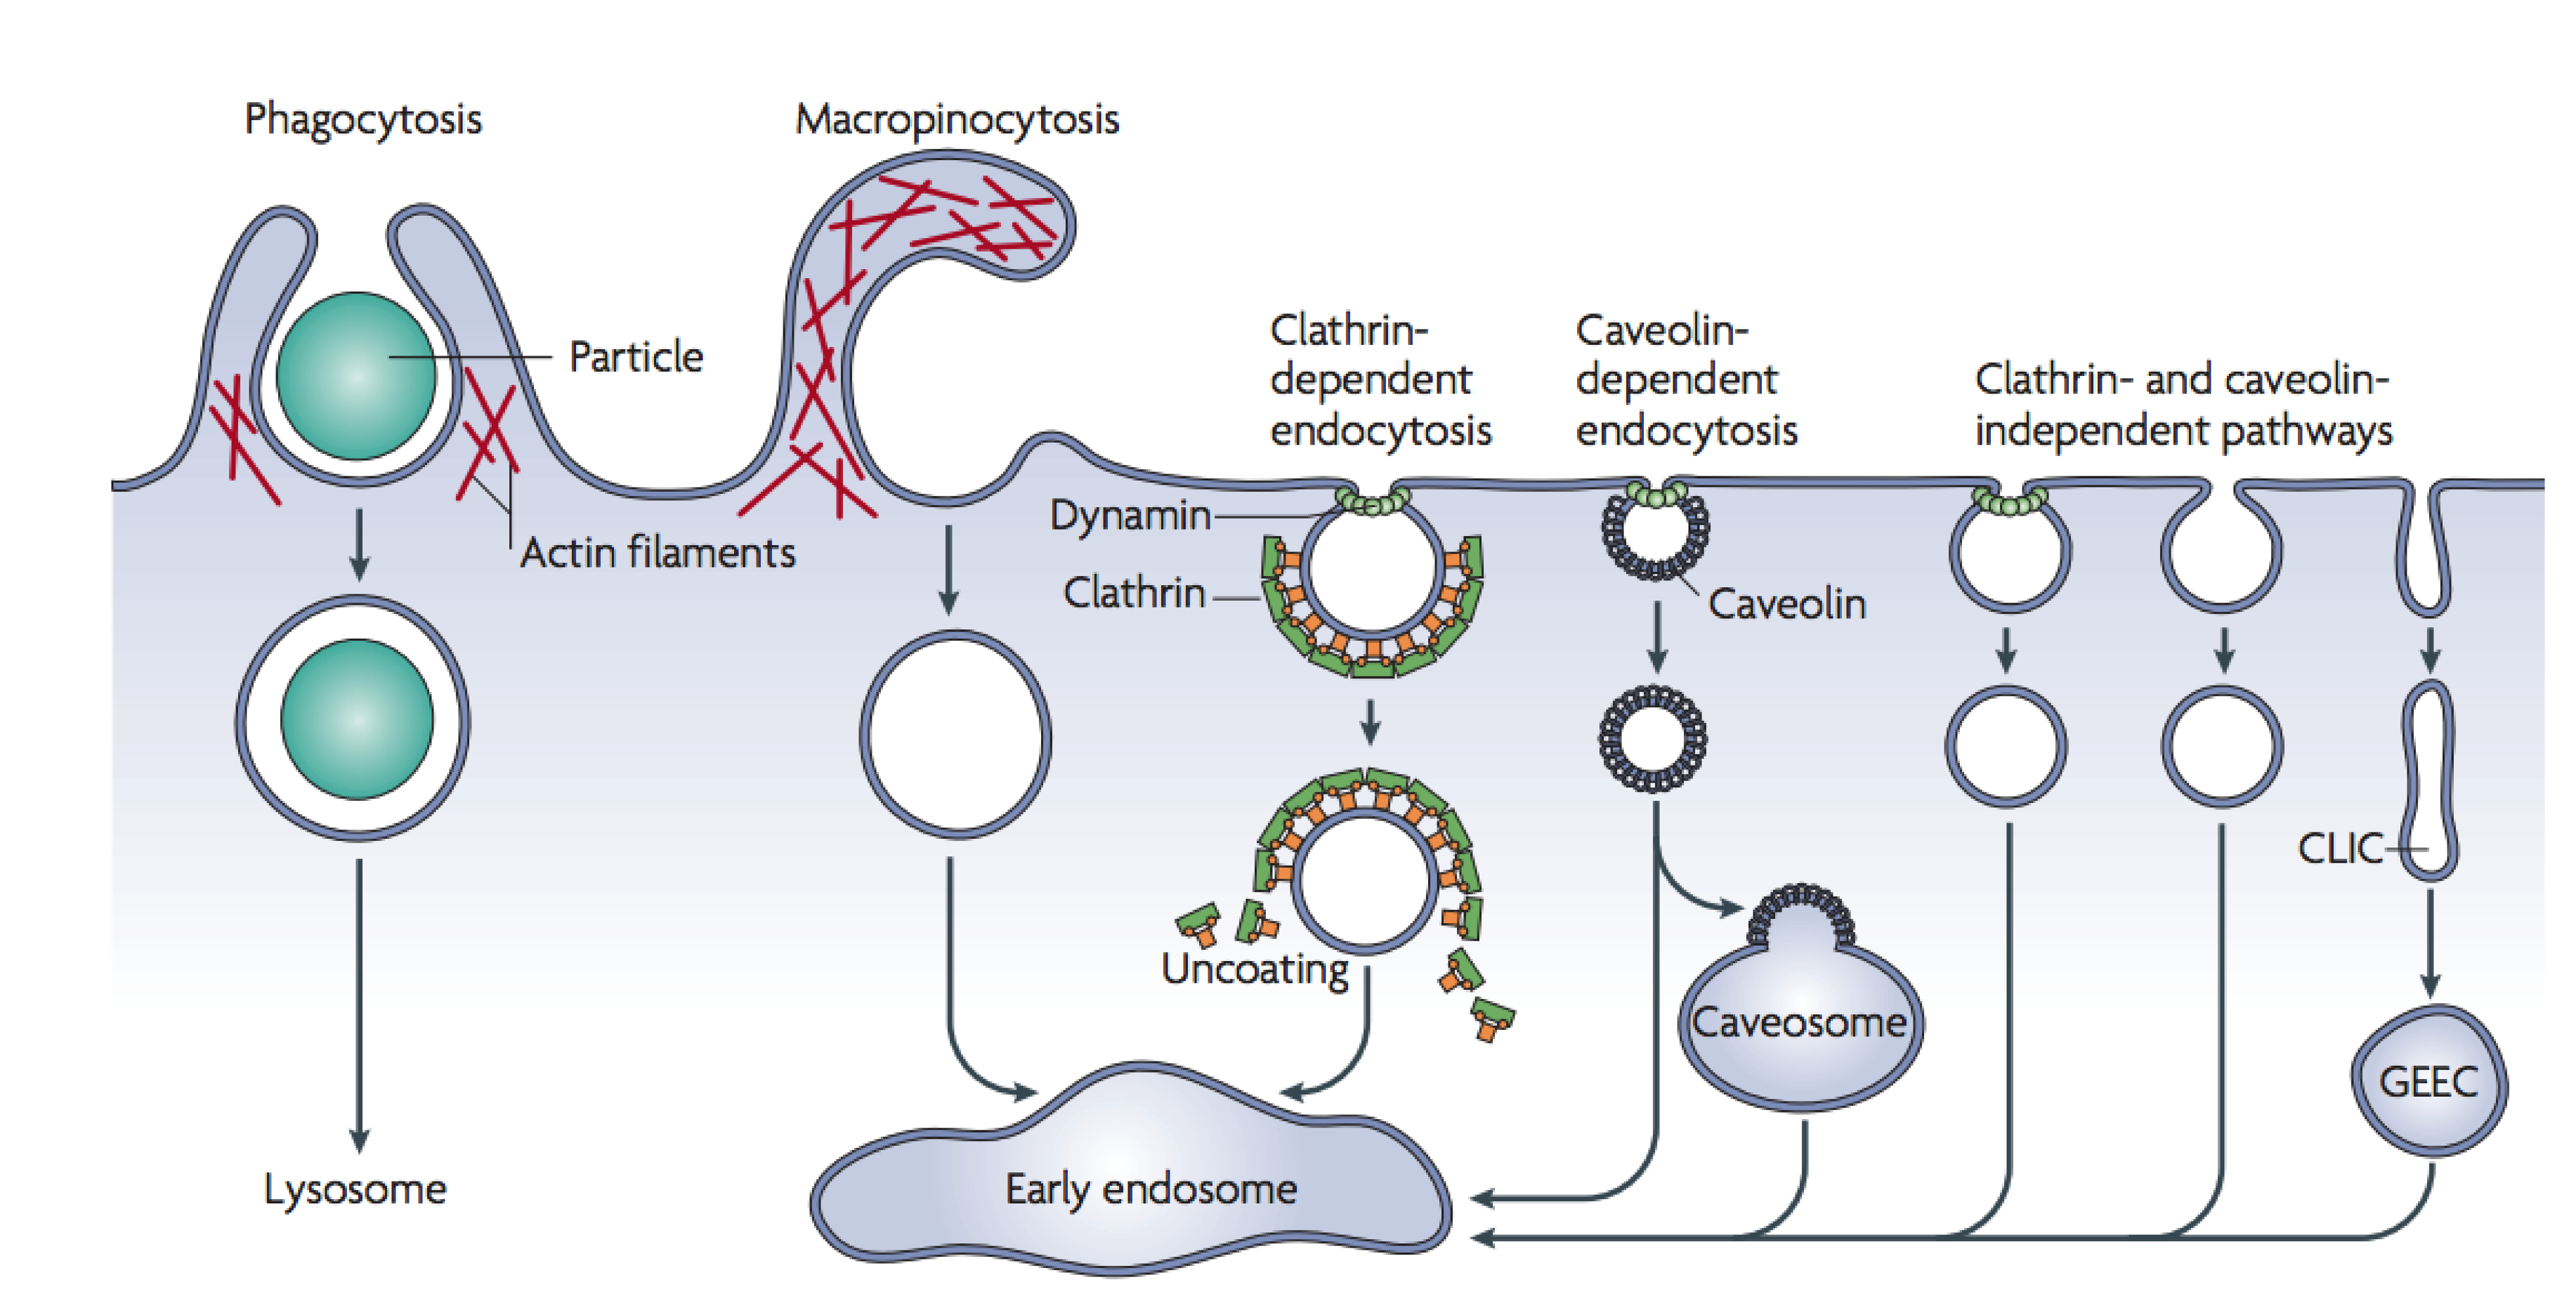
\includegraphics[width=14cm, height=16cm, keepaspectratio]{figures/intro/Fig1_mayor}
	\caption[Endocytic pathways in cells]
	{Some of the endocytic pathways in mammalian cells. Large particles are incorporated by phagocytosis, bulk fluid by macropinocytosis. A large array of cargo is taken into the cell via CME and calveolin-dependent endocytosis. Vesicles formed by these pathways are targeted to the early endosome. Clathrin and calveolin-independent pathways incorporate cargo and involve different geometries, including tubular "clathrin- and dynamin-independent carriers" (CLIC), that arrive at "GPI-anchored protein enriched early endosomes" (GEEC), before they are transported to endosomes.  \textit{Reprinted by permission from Springer Nature: Nature Reviews Molecular Cell Biology (Mayor and Pagano, 2007), copyright (2007)}
		\label{intro_mayor}}
\end{figure}

 into the cell (Bitsikas, Corrêa and Nichols, 2014). It was first identified when studying yolk uptake in mosquitos, and ultrastructural studies of their oocytes (where frequency of uptake events is high enough to be easily studied) identified a bristly coat formation inside the cell membrane and similarly bristly vesicles (Fig.\ref{intro_clathrin}). These vesicles then lost the bristly coat and fused to eventually form yolk bodies in the mature oocyte (Roth and Porter, 1964). The bristle was noted in several cell types, and later identified as a lattice of a single highly conserved protein (Pearse, 1976). This protein was named Clathrin, derived from the latin word for lattice. 


\vspace{5mm}
Clathrin is formed of light and heavy chains incorporated into a triskelion (Ungewickell and Branton, 1981) that assembles into closed hexagonal and pentagonal structures on the inner leaflet of the plasma membrane (Fig.\ref{intro_clathrin}). CME has, since four decades ago, been recognized has an ubiquitous mechanism of membrane uptake in cell types ranging from the frog presynaptic membrane (Heuser and Reese, 1973) to rat vas deferens (Friend and Farquhar, 1967). Clathrin also localizes to the trans-golgi network (TGN): these clathrin-coated vesicles mediate traffic from the TGN to the endosome. Specification of vesicle cargo and targeting to different cellular compartments is achieved by clathrin interaction with specialized adaptor proteins like the adaptor protein complexes (AP), which specifies Golgi-to-early endosome traffic, while Golgi-localized gamma-adaptin (GGA) complexes specify Golgi-to-late endosome traffic (Payne, 2013). 



\begin{figure}[H]
\centering
%\hspace*{-0.6cm}
	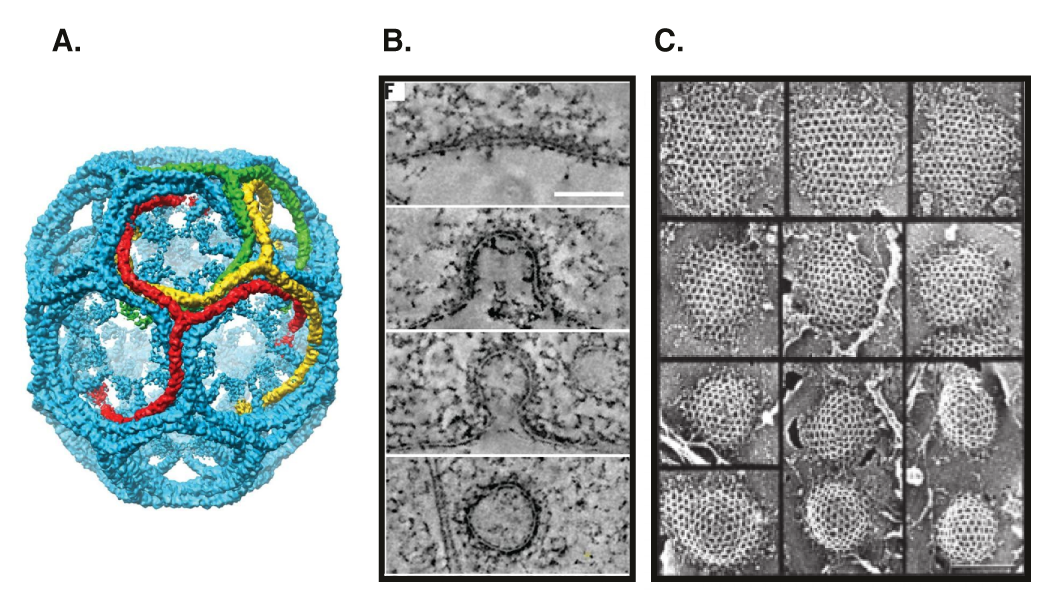
\includegraphics[width=13cm, height=16cm, keepaspectratio]{figures/intro/clathrin2}
	\caption[Endocytic pathways in cells]
	{ A: Model for a clathrin-cated vesicle based on cryo electron microscopy.Three individual triskeleons are highlighted. \textit{Reprinted wjth permission from Springer Nature: Nature. Molecular model for a complete clathrin lattice from electron cryomicroscopy,  Fotin et al., Copyright 2004}.
		B:   Slices through tomograms of clathrin-coated pits in different stages of invagination. \textit{From Avinoam et al, Science 2016. Reprinted with permission from AAAS.}
		C: Freeze-etch view of plasma membrane of mouse fibroblast showing a range of clathrin lattices. \textit{Republished with permission from CCC, from Three-dimensional visualization of coated vesicle formation in fibroblasts, Heuser, JCB 84, 1980 }
		\label{intro_clathrin}}
\end{figure}

	
\section{CME in mammalian and yeast cells }
		\subsection{Clathrin is required for mammalian CME}
The clathrin lattice was speculated as responsible for remodelling the plasma membrane and selecting cargo in the first papers that noted the “bristly” coat (Roth and Porter, 1964; Kanaseki and Kadota, 1969).  In multicellular organisms like \textit{Caenorhabditis elegans}, clathrin depleted by RNAi results in decreased endocytic uptake in oocytes and dead progeny (Grant and Hirsh, 1999). In \textit{Drosophila melanogaster}, deletion of clathrin heavy chain results in embryonic lethality (Bazinet et al., 1993). Knock-down of the heavy chain by RNAi in Hela cells results in decrease in endocytosis by 80\% (Huang et al., 2004). Essentially, endocytosis fails in the absence of clathrin in multicellular organisms. How exactly the clathrin coat shapes the progression of endocytosis has been heavily debated, but its involvement itself has not. 

\vspace{5mm}
Early work in yeast revealed that clathrin is not necessary for endocytosis (Payne and Schekman, 1985). Loss of clathrin only changes the size of the vesicles formed and leads to decrease in the number of established endocytic sites (Kaksonen, Toret and Drubin, 2005; Kukulski et al., 2016). Clathrin appears to affect establishment of sites and regulation of scission, but is not necessary for membrane invagination. It is now apparent that though the mammalian and yeast systems are mechanistically similar and most of the yeast endocytic proteins have mammalian homologues (Weinberg and Drubin, 2012), there are some significant differences.


		\subsection{Actin forces are required for yeast CME}
A single gene in yeast encodes the highly abundant actin protein, which is essential for cell survival (Koteliansky et al., 1979; Greer and Schekman, 1982). Organization of actin into axial filaments and cortical patches polarized to emerging buds was first described using phalloidin staining in fixed \textit{S.cervisiae} (Adams and Pringle, 1984). These patches were later established as dynamic endocytic sites by observing co-localization with other endocytic proteins (Kübler et al., 1993). While the mammalian CME is heavily dependent on clathrin for invagination, the yeast system relies on actin filament polymerization and depolymerization for membrane invagination: disrupting actin filament dynamics blocks endocytosis (Kübler et al., 1993). 



	
		\subsection{CME in yeast is highly regular}
	In yeast, over fifty proteins are recruited, interact, and disassemble during the endocytic process. In mammals as well as in yeast, proteins that arrive at an endocytic site can be assigned into different modules according to their relative time of recruitment and function (Fig.\ref{intro_endpathway}). 

\vspace{5mm}
An initiation phase assembles coat proteins on the plasma membrane and establishes an endocytic site. The early proteins involved in the initiation phase are highly variable in both recruitment as well as time spent at sites. Initiation is followed by a very stereotypic sequence of events that assembles coat proteins, nucleates actin, organizes the actin network, invaginates a membrane tube, and finally severs the membrane to produce vesicles (Kaksonen, Toret and Drubin, 2005). While the entire process of initiation through scission occurs over a period of about a minute, once membrane invagination begins, inward movement and consecutive scission occurs in under fifteen seconds. This indicates tight regulation of the post-initiation sequence of events in the endocytic timeline. 

		\vspace{5mm}
Sterotypicity of the later stages of yeast endocytosis allows us to average the behaviour of a particular protein from multiple endocytic sites. Tracking the behaviour and organization of these proteins has led to a remarkably detailed understanding of the spatial and temporal regulation of endocytosis in yeast (Kaksonen, Toret and Drubin, 2005; Picco et al., 2015; Mund et al., 2018). The different stages of endocytosis are discussed below. 

		
 


			\subsubsection{Early initiation phase}
The initiation phase establishes endocytic sites and selects cargo (Brach et al., 2014). Deletion of an entire seven protein set of early endocytic proteins (Ede1, Syp1, Yap1801/1802, Apl1, Pal1, Pal2) does not prevent endocytosis. It seems that the initiation of endocytosis in yeast is independent of the recruitment of any one protein, and is likely a result of several different cooperative or independent factors (Brach et al., 2014). This could give the process robustness in the absence of alternate pathways for uptake of essential nutrients and signals. The variability in this phase could also provide a “check-point”, to ensure that sufficient cargo is loaded (Weinberg and Drubin, 2012) before later (energy consuming) phases are triggered. 


			
			\subsubsection{Coat module}
Coat proteins serve to template later-arriving proteins (Mund et al., 2018), as well as form the link between the actin network and membrane (Skruzny et al., 2012). Clathrin adaptors and the clathrin triskelion are not necessary for the progression of sites. Deletion of coat proteins Sla2 (Hip1R homologue) and Ent1 (Epsin homologue) results in what is known as an “uncoupling” phenotype. In these cells, actin polymerizes at the plasma membrane, but the membrane is decoupled from actin forces. This results in actin “flames” at cortical patches without membrane bending (Kaksonen, Sun and Drubin, 2003; Skruzny et al., 2012). A complex formed between Sla1, Pan1 and End3, which links the early coat to other coat proteins and polymerized actin, is involved in actin regulation itself, and connects vesicles to actin cables and endosomes (Wendland and Emr, 1998; Sun et al., 2015; Toshima et al., 2016). These proteins move inward into the cytoplasm with the membrane invagination
			



			\subsubsection{Actin module}
Once coat proteins are assembled, proteins that nucleate and organize a branched actin network are recruited. Actin filaments are nucleated by the Arp2/3 complex, acting in concert with actin nucleation promoting factors (NPFs): Wiscott-Aldrich syndrome protein (WASP) homologue Las17, type 1 myosins Myo3 and Myo5, intersectin homologue Pan1, and actin binding protein Abp1. Las17 is a potent actin nucleator, without which endocytosis essentially fails (Yidi Sun, 2006). Myo3/5 are non-processive motor proteins that interact with and can translocate actin filaments, but whose mechanistic contribution to endocytosis is unknown. Deletion of either Myo5 or Myo3 has subtle phenotypes, but deletion of both effectively blocked endocytosis (Yidi Sun, 2006). Abp1 binds actin filaments and is thought to activate the Arp2/3 complex. Without Abp1, cells are viable, but coat proteins persist on vesicles instead of disassembling after membrane scission. This suggests that Abp1 helps to dismantle the endocytic machinery. In support of this role, recruitment of late-stage enzymes like Ark1 and Prk1 that recycle endocytic proteins to membrane invaginations require Abp1. 


%\newpage



	\begin{figure}[H]
	\centering
%	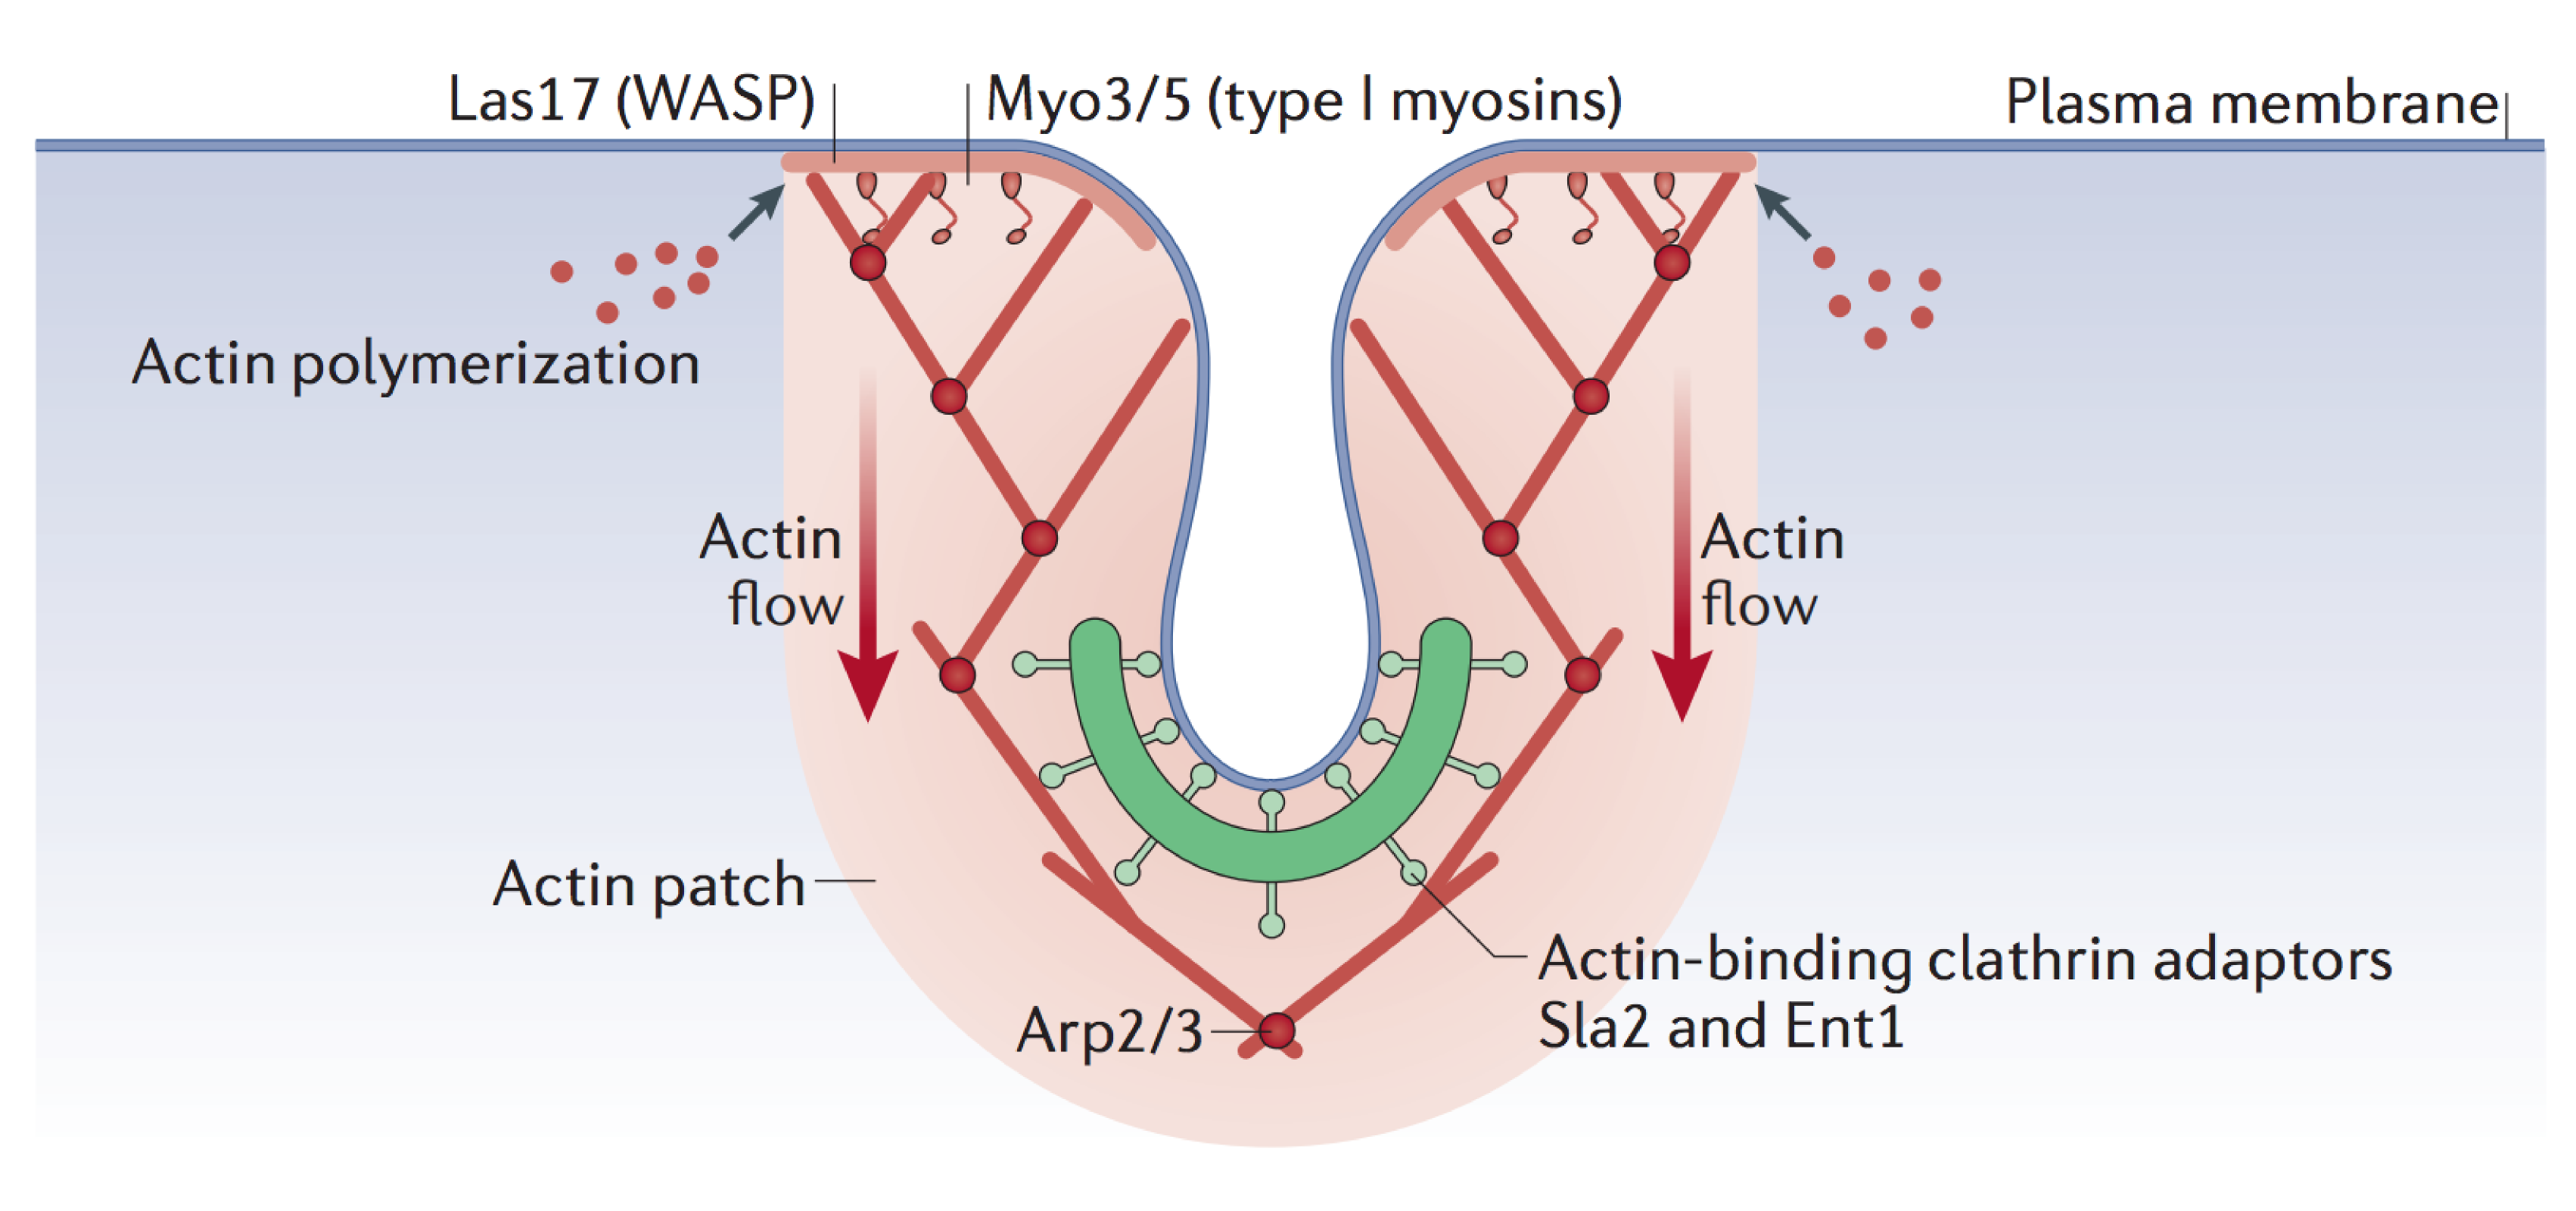
\includegraphics[scale=0.5]{figures/intro/actin_kaksonen}
		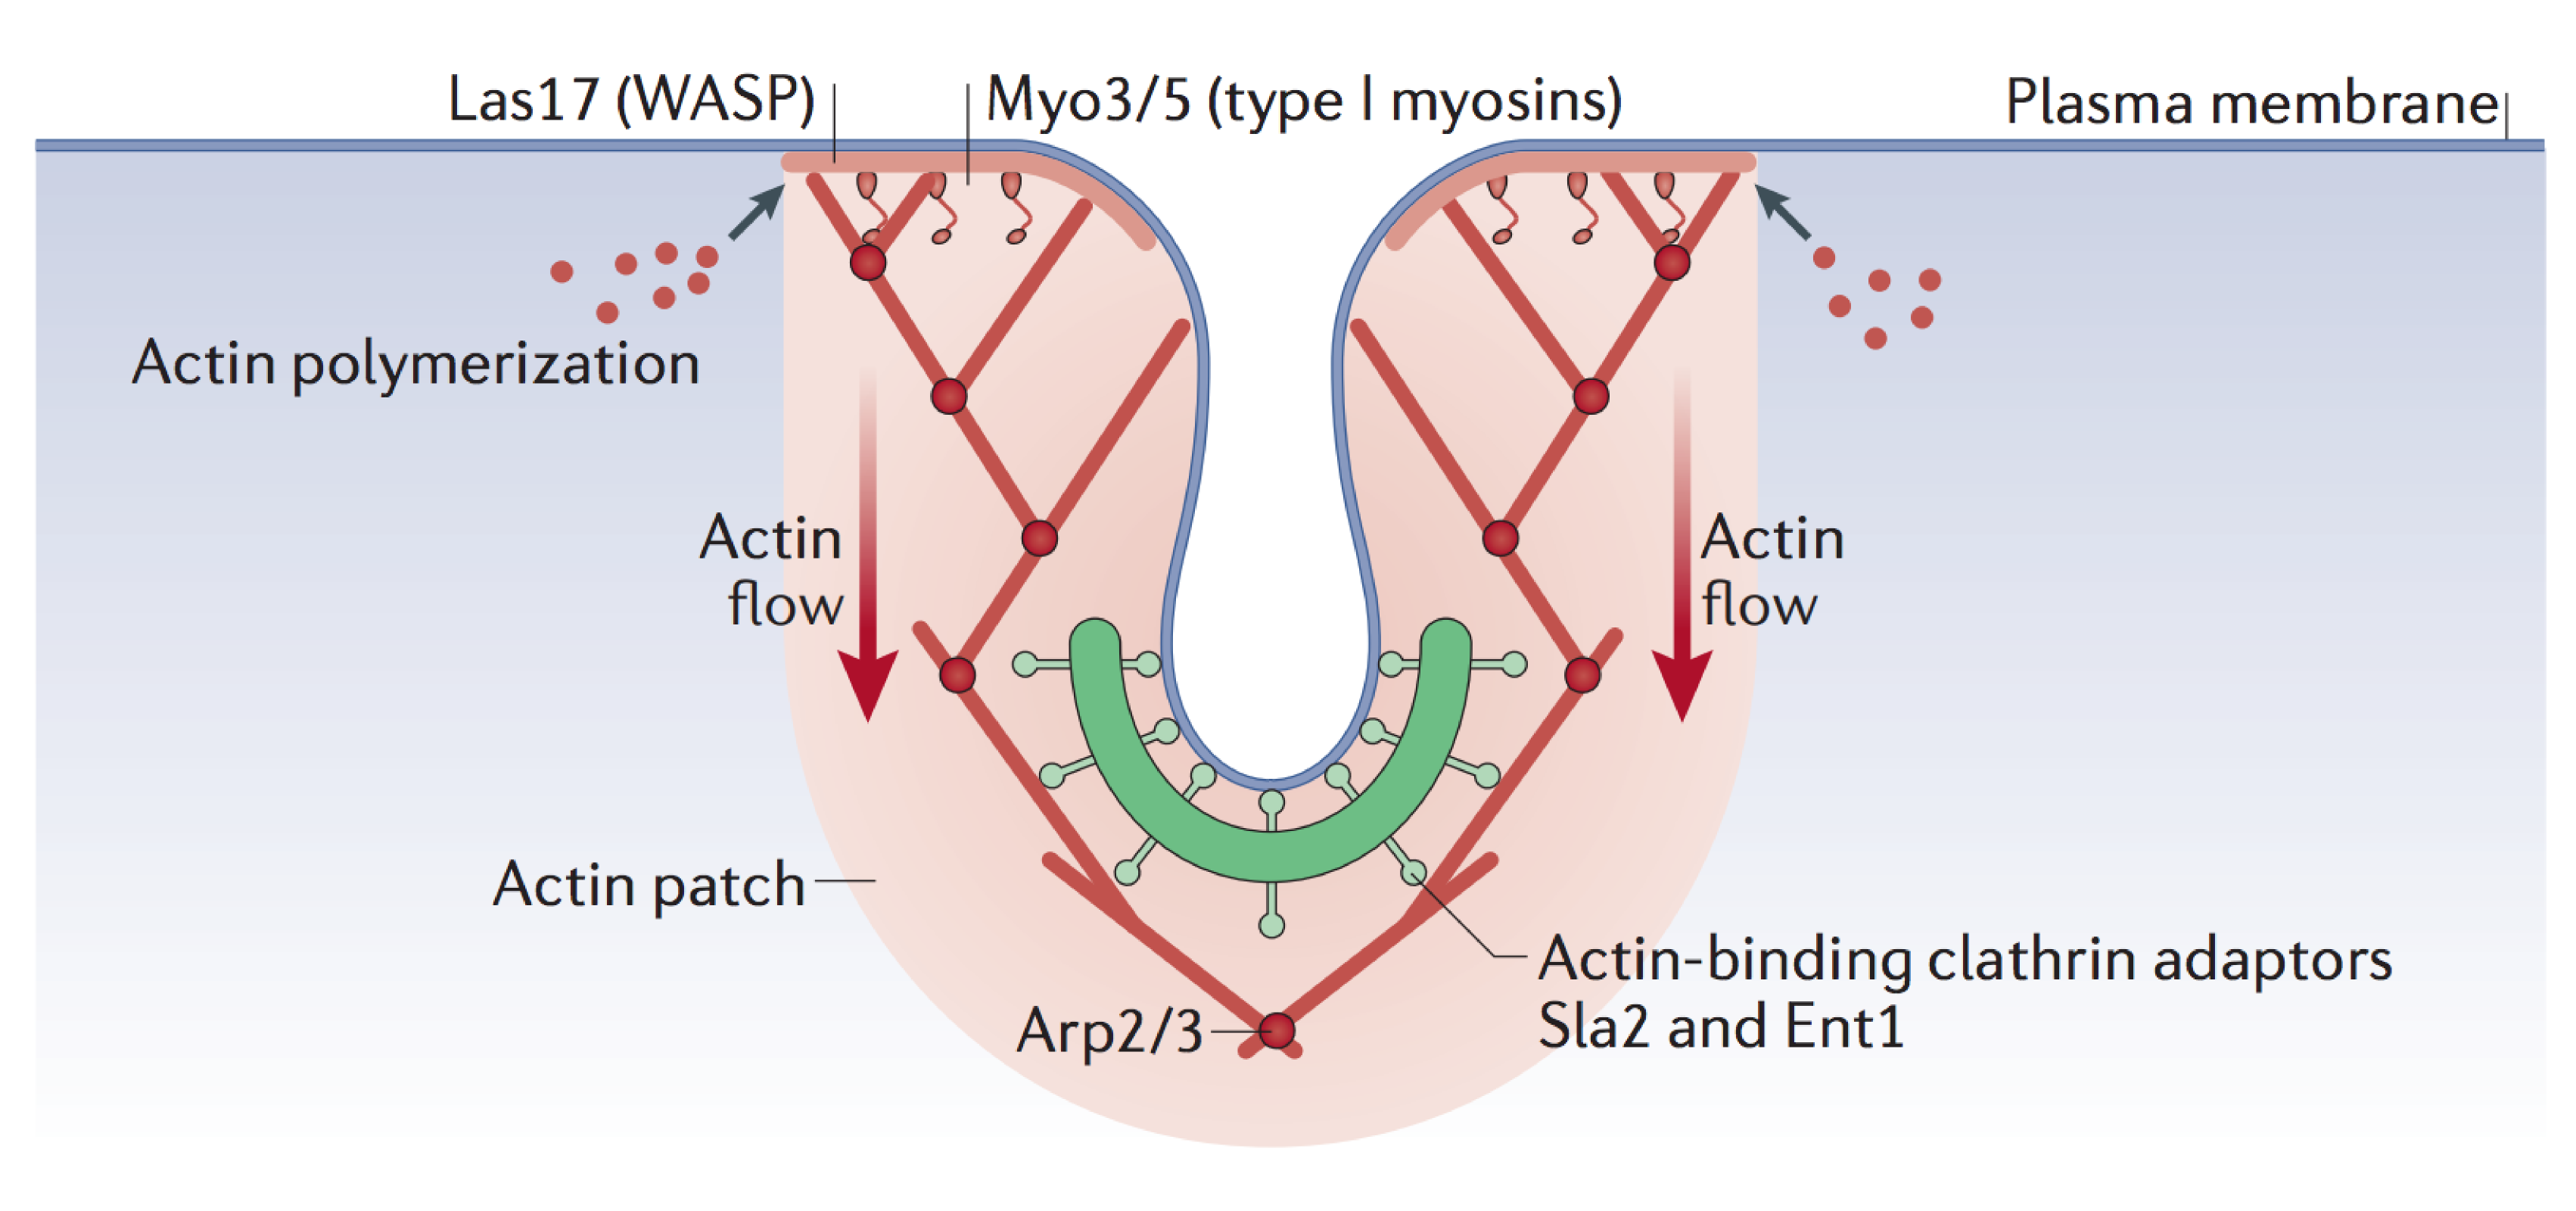
\includegraphics[width=14cm, height=15cm, keepaspectratio]{figures/intro/actin_kaksonen}
	\caption[Actin network in endocytosis]
	{The model for actin-driven membrane invagination in yeast. Actin filaments are nucleated around the base of the invagination by the Arp2/3 complex, which is activated by Las17 and Myo3/5. Actin polymerization at the base pushes the actin network inward into the cell (actin flow). The actin network is coupled to the membrane by Sla2 and Ent1, which is also pulled inward with the actin network as actin filaments polymerize. \textit{Reprinted by permission from Springer Nature: Nature Reviews Molecular Cell Biology (Kaksonen and Roux, 2018), copyright (2018)
	\label{intro_actin_netork}}}
\end{figure}


		\vspace{5mm}
Bbc1, Bzz1, and Vrp1 are other actin associated proteins that are recruited within the actin module. Bbc1 is known to inhibit Las17 NPF activity: its deletion accumulates actin at endocytic sites(Picco et al., 2018). Bzz1, an F-BAR protein, relieves Las17 of NPF activity inhibition by Sla1(Yidi Sun, 2006). Vrp1 acts in concert with myosins and Las17 to stimulate the Arp2/3 complex (Anderson et al., 1998; Wong et al., 2010). 

			\vspace{5mm}
Once NPFs and WASP/Myo proteins are recruited, Arp2/3 is recruited and actin polymerization begins. Actin crosslinkers like Sac6 and Scp1, capping protein complexes like Cap1/Cap2, Aip1/Cofilin, Abp1/Aim3 are recruited at this time. This begins the invagination of membrane. Actin monomers are added at the base of the invagination, and the actin network is linked to the membrane via coat proteins Sla2 and Ent1. As actin polymerization progresses, the entire actin network is pushed inwards, taking the membrane along with it (Picco et al., 2015).	

\newpage
\begin{figure}[H]
	\centering
	\hspace{-1.5cm}
%	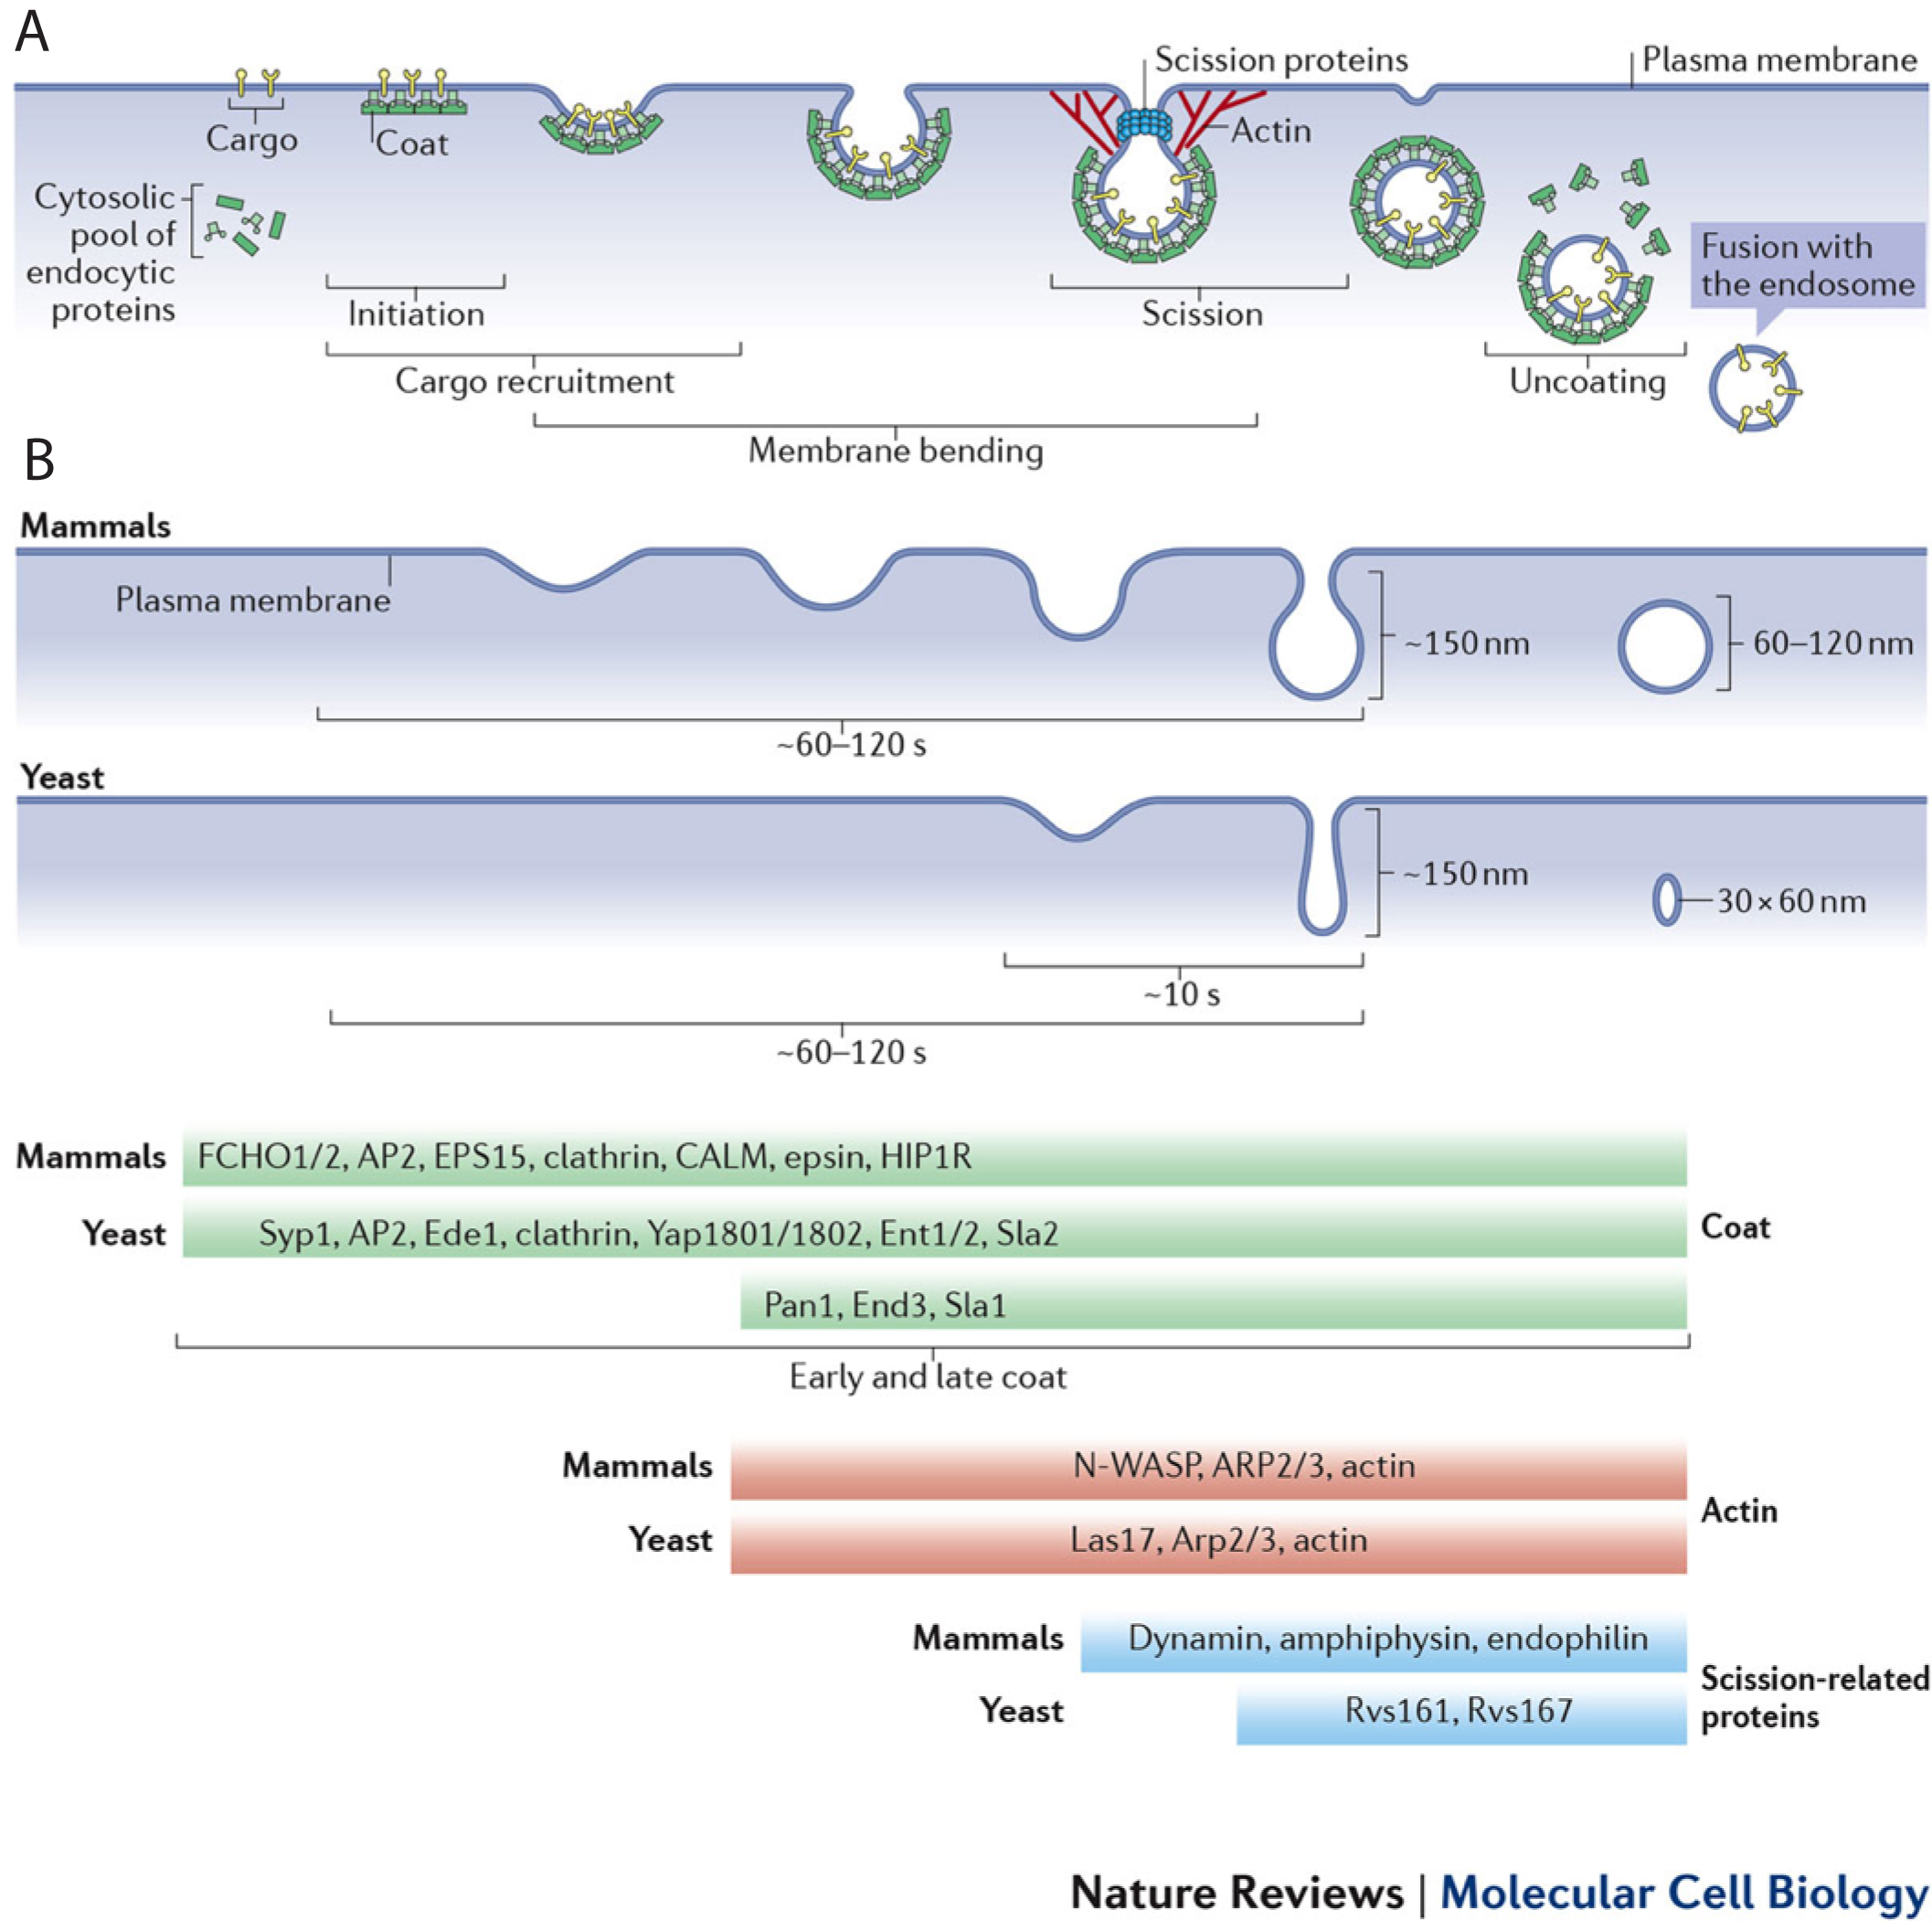
\includegraphics[scale=0.8]{figures/intro/Fig2_kaksonen}
		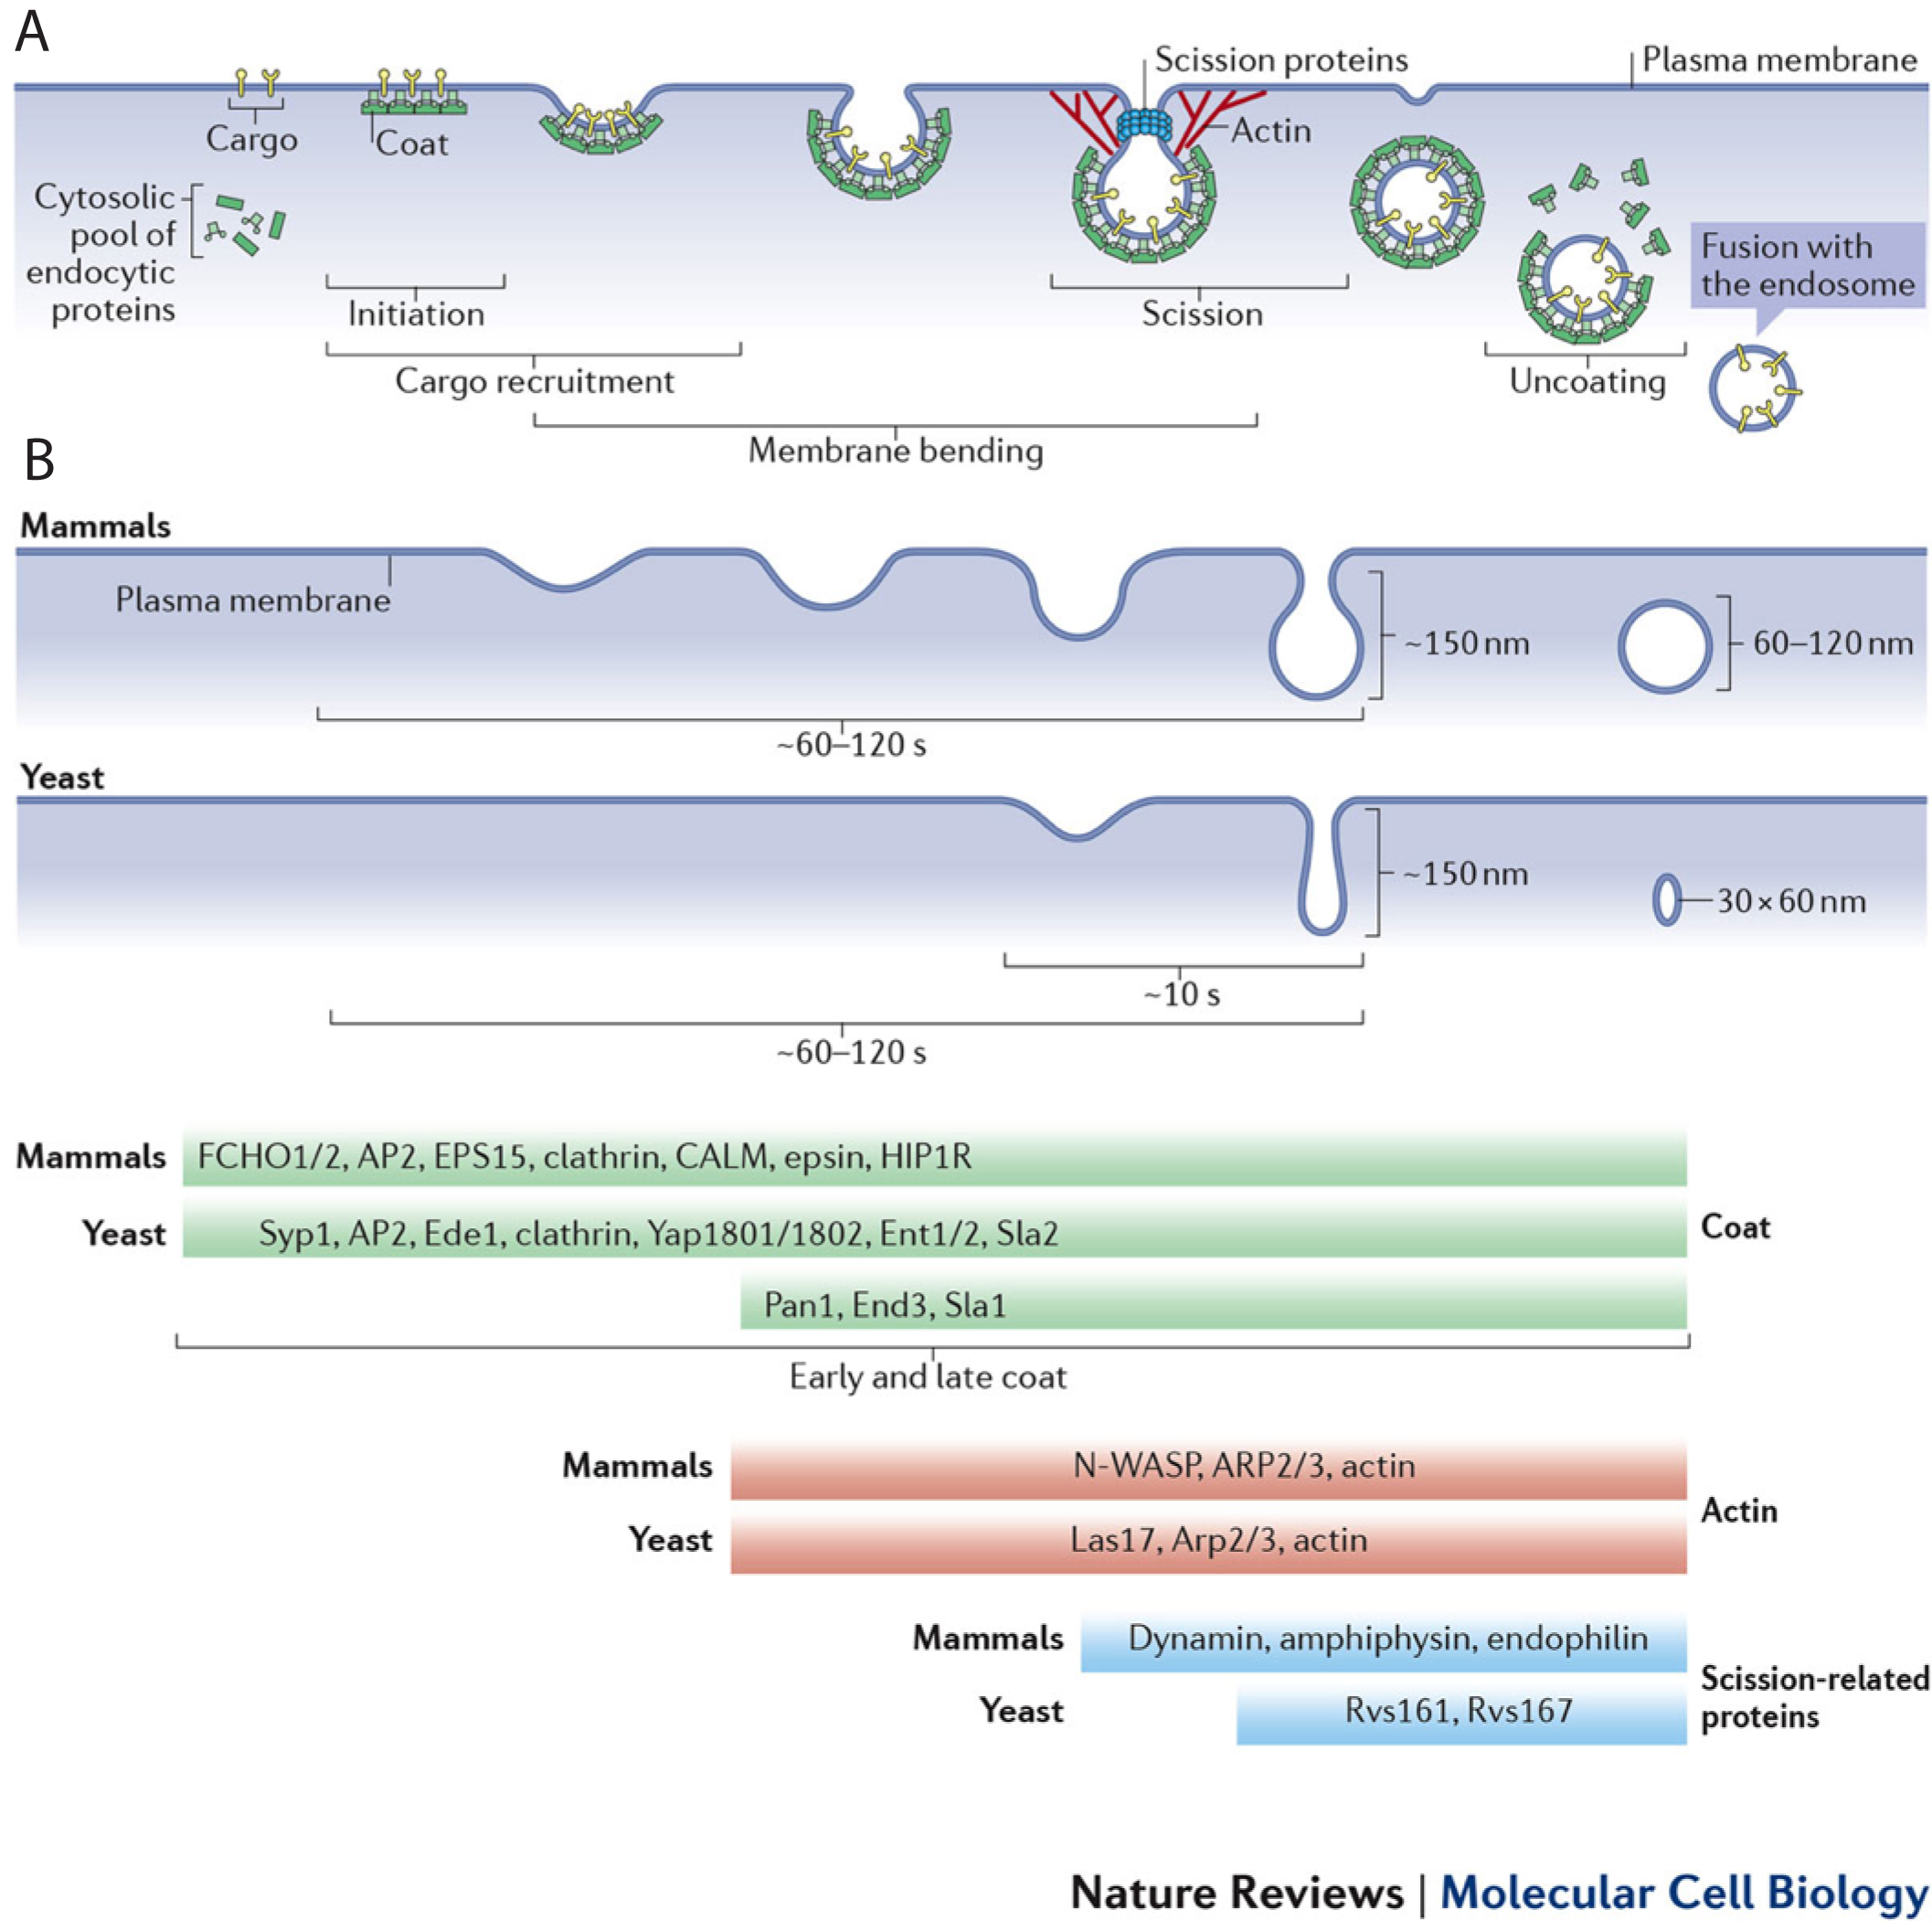
\includegraphics[width=15cm, height=28cm, keepaspectratio]{figures/intro/Fig2_kaksonen}
	\caption[Endocytic pathway in mammalian and yeast cells]
	{A: Proteins involved in endocytosis are recruited from a cytoplasmic pool. Initiation of an endocytic event and cargo recruitment is followed by membrane bending. Membrane scission eventually forms a vesicle that releases its components, allowing it to be transported down the trafficking pathway. B: Membrane invagination in mammalian cells results in wider vesicles than in yeast cells. Proteins that are involved can be grouped based on their function in the endocytic pathway. Shown here are the main proteins involved that are conserved between the two species. 
		\textit{Reprinted by permission from Springer Nature: Nature Reviews Molecular Cell Biology (Kaksonen and Roux, 2018), copyright (2018)}
		\label{intro_endpathway}}
\end{figure}

\newpage
			\subsubsection{Scission module}
When the membrane invagination grows about 140nm, scission occurs, forming a vesicle. What actually causes scission in yeast is not yet determined (see Section\ref{yeast_scission}).
The role of the dynamin in yeast endocytosis is unclear so far. N-BAR domain complex Rvs161/Rvs167 (Rvs) is recruited in the late stage of invagination, and membrane scission occurs shortly after it arrives (Kukulski et al., 2012; Picco et al., 2015). 
\vspace{5mm}
Coat proteins and the actin network are finally disassembled from the vesicle after scission and the nascent vesicle is transported into the cell. Disassembly of coat components are regulated by kinases Ark1/Prk1 that phosphorylate several coat proteins like Sla1, Sla2, and Pan1. Glc17 and its adaptor Scd5 likely dephosphorylate these proteins so that can be incorporated into a new endocytic event. How the actin machinery is disassembled is not clear. The actin network is constantly assembled and disassembled throughout endocytosis, and growth of the actin network likely indicates that the rate of assembly of filaments is higher than disassembly. NPFs Myosins and Las17 stop being recruited to endocytic sites seconds before scission occurs (Picco et al, 2015), so actin network disassembly is likely a result of a change in the ratio of assembly/ disassembly of the actin network. Disassembly is likely caused by increased rate of disassembly of actin, compared to assembly. 




		
		\newpage
\subsection{Membrane scission in mammalian cells}
		\subsubsection{Scission is dependent on dynamin} 
In mammalian cells, endocytic membrane scission is primarily effected by the GTPase dynamin. Dynamin was originally discovered as mediating interactions between microtubules (Shpetner and Vallee, 1989). It is now known to play a pivotal role in membrane scission and fusion events at many different cellular organelles. The importance of dynamin in endocytosis was demonstrated in a temperature-sensitive mutant of the Drosophila shibire gene, which results in paralysis of flies at the non-permissive temperature. These flies fail to form synaptic vesicles (Grigliatti et al., 1973; Poodry and Edgar, 1979; van der Bliek and Meyerowrtz, 1991). Shibire codes for multiple isoforms of dynamin that are differentially expressed across the organism (Chen et al., 1991). Knock-down of dynamin isoforms disrupts vesicle-formation after invagination, resulting in accumulation of a large number of long membrane tubes (Ferguson et al., 2009). 

		\subsubsection{Dynamin is an oligomeric GTPase}
%		PIP\textsubscript{2}
Dynamins consist of a GTPase domain, a stalk region, a bundle signalling element that acts as the linker between the GTPase domain and stalk, a phosphatidylinositol (4,5)-bisphosphate (PtdIns(4,5)P2 , henceforth 	PIP\textsubscript{2})- binding pleckstrin homology domain (PH) domain and a proline rich domain (PRD) that extends beyond the GTPase domain (Antonny et al., 2016). \textit{In vitro}, dynamin oligomerizes into helical structures with the PH domain apposed against the membrane, and the GTPase domain facing away from the membrane (Sweitzer and Hinshaw, 1998; Zhang and Hinshaw, 2001). As depicted in Fig\ref{intro_dynamin_scission}, dynamin within the helical structure undergoes conformation changes upon GTP hydrolysis that constricts the helix as well as the membrane tube under it, collapsing the inner leaflet of the bilayer membrane into a hemi-fission state, resulting in membrane fission (Zhao et al., 2016). Disruption of its GTPase activity results in membrane tubes that accumulate dynamin and fail to undergo scission (Takei et al., 1995; David et al., 1996; Ringstad, Nemoto and De Camilli, 1997).

		
	\begin{figure}[H]
			\centering
			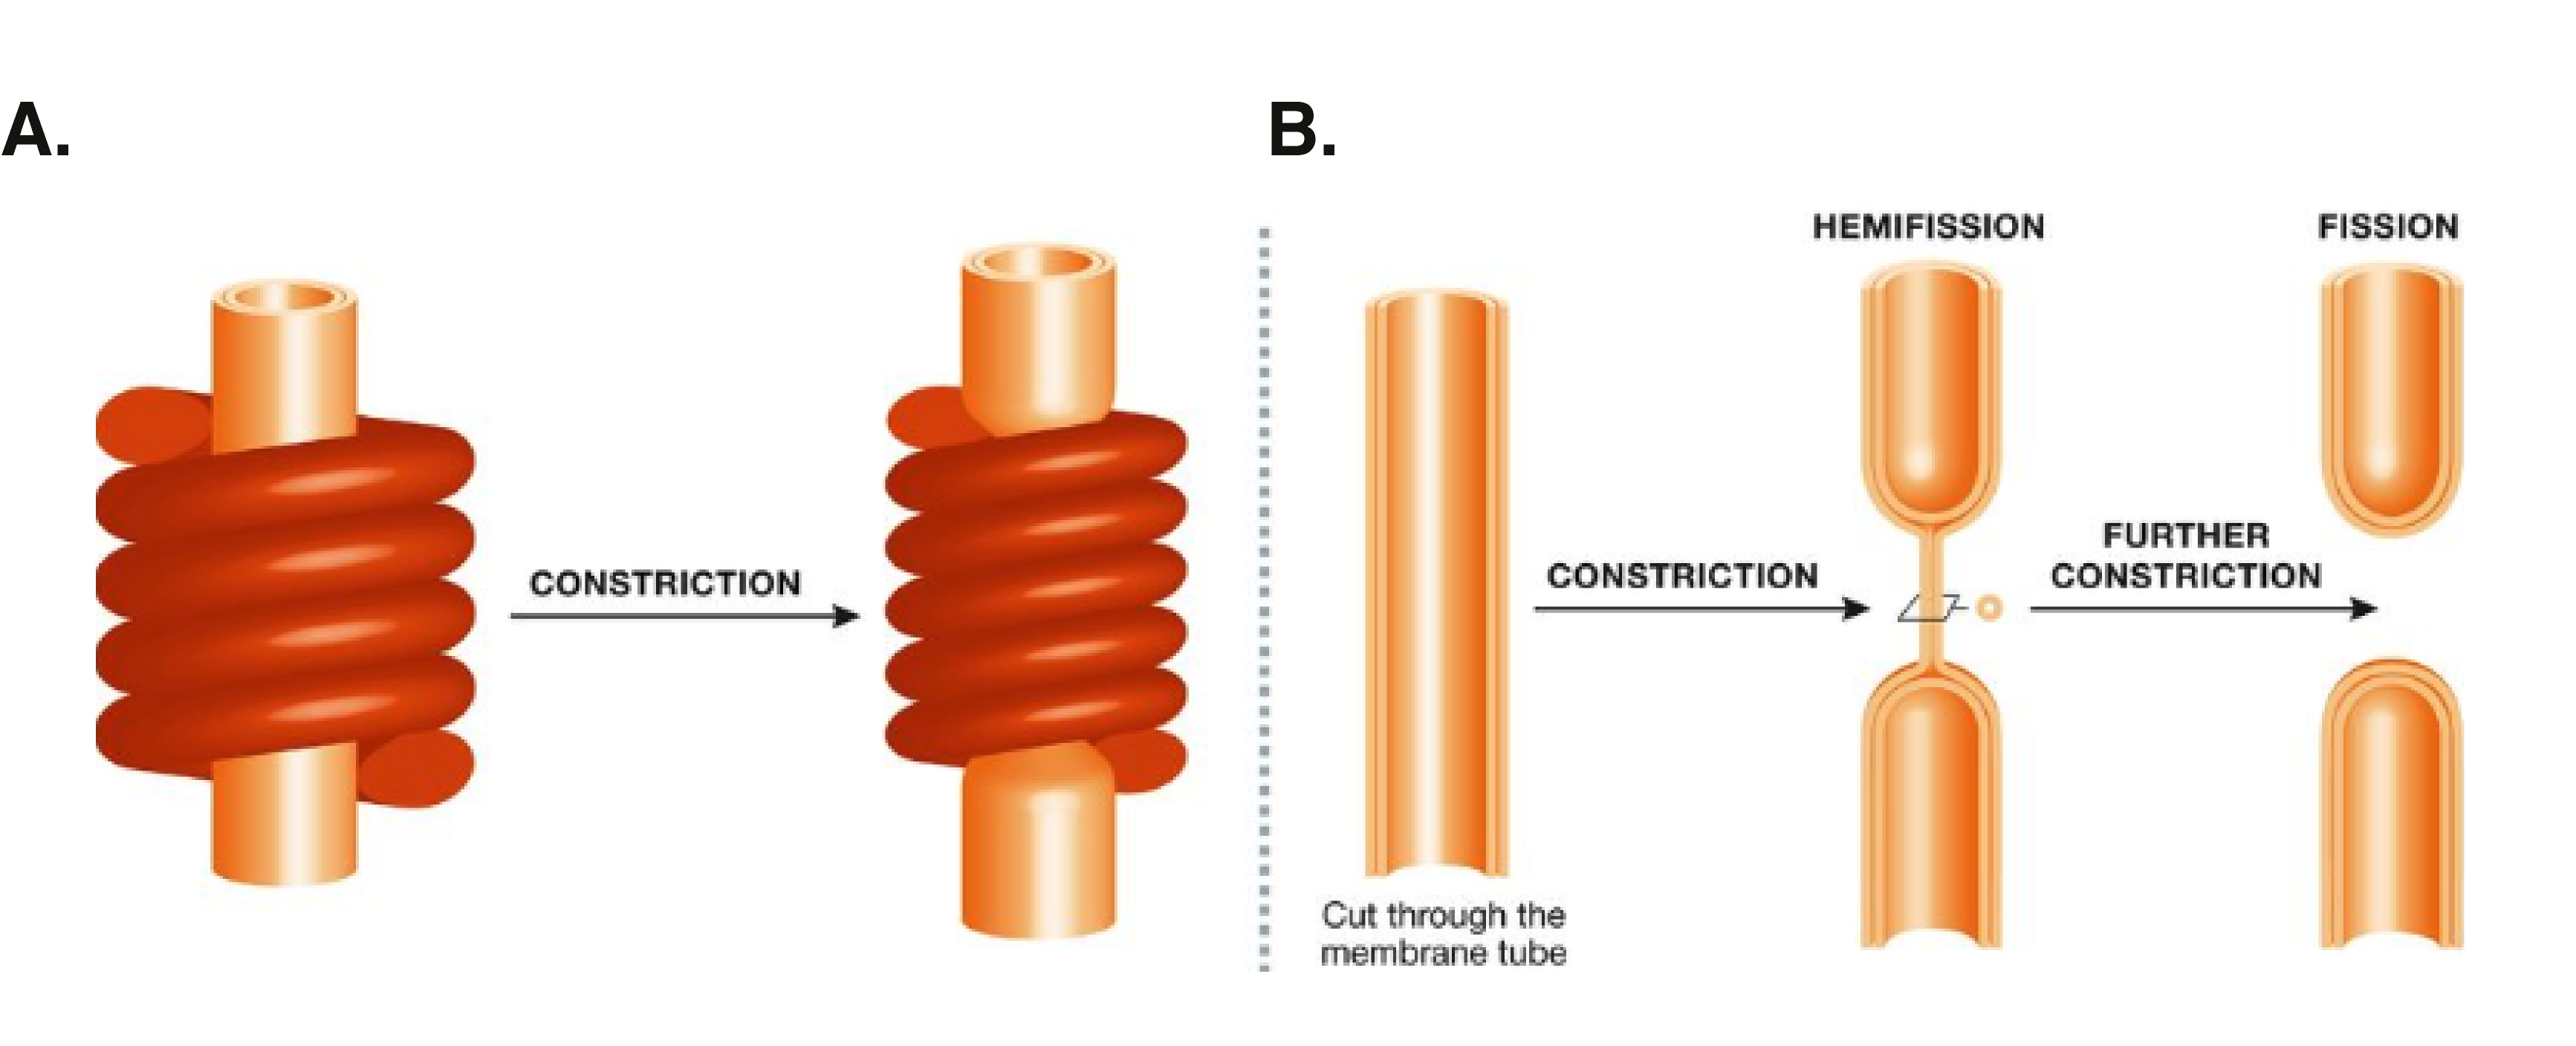
\includegraphics[scale=0.545]{figures/intro/dynamin_3}
\caption[Dynamin forms a scaffold]
					{Dynamin-mediated membrane constriction model. Dynamin forms a helical structure around the membrane. GTP hydrolysis constricts the helix and the membrane into first a hemifission state and then to fission.
					\textit{Reproduced from Antonny et al, under Creative Commons Cttribution Non-Commercial No Derivatives Licence CC BY-NC-ND}
		\label{intro_dynamin_scission}}
		\end{figure}


%(Adam et al., 2015) under creative commons licence \href{https://creativecommons.org/licenses/by/4.0/}{CC BY 4.0}}}

		\subsubsection{Dynamin interacts with BAR proteins to cause scission}
\textit{In vivo}, dynamin arrives at clathrin-coated pits via interaction with BAR proteins endophilin and amphiphysin (Ferguson et al., 2009). BAR domain proteins form intrinsically curved protein dimers. In addition to the BAR domain, most BAR proteins have additional motifs that mediate their interaction with membranes or other proteins. Some BAR proteins have an N-terminal amphiphatic helix (N-helix) that is inserted into the membrane bilayer.  Others have phosphoinositide binding motifs like phox or pleckstrin homology (PH) domains, which direct BAR proteins to specific lipids within membranes. Some BAR proteins contain Src homology 3 (SH3) domains that mediate protein-protein interaction. These SH3 regions act as a scaffold for the proline-rich domains (PRD) of dynamin (Grabs et al., 1997). 



		\subsubsection{Dynamin and BAR proteins interact via PRD and SH3 regions }
Dynamin’s PRD interacts with the SH3 domains of BAR proteins endophilin and amphiphysin (Grabs et al., 1997; Cestra et al., 1999; Farsad et al., 2001; Meinecke et al., 2013). Endophilin and dynamin appear to help recruit each other: Endophilin recruitment is reduced in the absence of dynamin, and vice-versa. Interaction with the endophilin BAR domain is also known to inhibit the GTPase action of dynamin (Farsad et al., 2001; Meinecke et al., 2013; Hohendahl et al., 2017). Meanwhile, amphiphysin levels are unchanged in absence of dynamin, while deletion of amphiphysin results in increased recruitment and prolonged lifetimes of dynamin and absence of membrane scission (Meinecke et al., 2013). These results suggest a role for amphiphysin for disassembly of dynamin involving GTP hydrolysis, and a role for endophilin in dynamin assembly. The mechanistic interplay between the two BAR proteins with dynamin is still debated, and the sequence of events that leads to membrane scission remains unclear (Neumann and Schmid, 2013; Hohendahl et al., 2017). Dynamin localization to clathrin-coated pits is not entirely dependent on BAR proteins, but both GTP hydrolysis and interaction with BAR proteins is necessary for efficient vesicle scission in mammalian cells (Shupliakov et al., 1997; Meinecke et al., 2013).


\label{key}

	\subsection{Membrane scission in yeast} \label{yeast_scission}
		\subsubsection{Yeast dynamin-like proteins}
In yeast, three dynamin-like large GTPases have been identified: Vps1, Dnm1, and Mgm1. Dnm1 and Mgm1 are involved in mitochondrial fission and fusion (Cerveny et al., 2007). Vps1 is essential for vacuolar protein sorting (Rothman et al., 1990). It is also involved in fission and fusion of vacuoles (Peters et al., 2004) and peroxisomes (Hoepfner et al., 2001), and is required for regulation of golgi to endosomal trafficking (Gurunathan, David and Gerst, 2002). Vps1 may also arrive at early endocytic events (Nannapaneni et al., 2010). None of the three yeast dynamins have the typical PH domain (Bui et al., 2012; Moustaq et al., 2016) that in mammals interacts with the lipid bilayer. Instead, an “InsertB” region likely performs the same function. Although yeast dynamins also do not have PRDs that could interact with the SH3 domains of yeast BAR proteins, Vps1 has been shown to interact with clathrin and other endocytic proteins (Yu, 2004; Nannapaneni et al., 2010; Goud Gadila et al., 2017), while other work has failed to observe localization of Vps1 at endocytic sites (Kishimoto et al., 2011; Goud Gadila et al., 2017). The role of Vps1 in endocytosis is thus not clear, but it is a candidate for the role of the canonical dynamin in CME.



		\subsubsection{Yeast BAR domain proteins Rvs161/167 regulate scission timing}
In yeast, the Amphiphysin/ Endophilin homologue is the heterodimeric complex Rvs161/167 (Friesen et al., 2006) (Rvs). Apart from an N-BAR domain, Rvs167 has a C-terminal SH3 domain. Rvs arrives at endocytic sites in the last stage of the endocytosis, and disassembles rapidly at the time of membrane scission (Picco et al., 2015). Deletion of Rvs results in failure of membrane scission in nearly 30\% of endocytic events (Kaksonen, Toret and Drubin, 2005). Scission failure is identified by the movement inwards of the endocytic protein coat into the cytoplasm, followed by its retraction back towards the cell wall, indicating a failure to form vesicles. No mutation of other endocytic proteins exhibits this phenotype. Electron microscopy has shown that in \textit{rvs167$\Delta$} cells, vesicles formed are smaller than in wild-type (WT) cells. This profile suggests that although Rvs is not necessary for scission, localization of the complex makes scission more efficient, and influences the invagination length at which scission occurs. Some mutations like that of the yeast Syndapin Bzz1 and Synaptojanin Inp52 in the background of \textit{rvs167$\Delta$} exacerbates the retraction phenotype (Kishimoto et al., 2011), suggesting that Rvs might act in concert with other proteins. 

\vspace{5mm}
		\subsubsection{Forces needed for membrane invagination and scission}
Forces are required to deform the membrane and pull it inward. In yeast, estimates of these forces are in the order of 1000 - 5000pN (Dmitrieff and Nédélec, 2015), influenced largely by the high turgor pressure within the cells. Intracellular forces of this magnitude are typically provided by components of the cytoskeletal network like microtubules and actin filaments. Disrupting formation of actin filaments completely disassembles the actin network and stops endocytosis (Kübler and Riezman, 1993; Aghamohammadazadeh and Ayscough, 2009). A substantial amount of the force required to pull up the membrane therefore comes from actin filament polymerization.

\vspace{5mm}
Actin monomers polymerize into filaments at the base of endocytic invaginations (Picco et al., 2015). Polymerization of actin filaments against a membrane can generate forces that push away this membrane, a mechanism that is employed across many organisms and cell types to produce movement. For example, the bacteria Listeria propels itself across its host cell by high-jacking the actin machinery of the host, and polymerizing an actin “comet tail” behind it. 

\vspace{5mm}
Simulations show that the highest force requirement for membrane deformation occurs at the beginning of membrane invagination (Dmitrieff and Nédélec, 2015). After a tubular structure is formed, a constant force can continue to pull the tube into the cytoplasm. At the time of scission, rather than a constantly growing actin network, NPF activity has essentially already plateaued (Picco et al., 2015), indicating there is likely less force exerted on the membrane at the time of scission than before scission. It is not clear what causes the final shape transition from membrane tube to vesicle.  

\vspace{5mm}
Rvs deletion appears to affect this transition, but its mechanistic contribution to this process has not been determined. Since yeast dynamins do not have PRDs, there is probably no interaction between dynamin and Rvs. A mechanism that does not involve PRD-SH3 interactions like in mammalian cells is therefore likely. Several scission models have been presented in the literature so far. They are described briefly below and in more detail in the results section (see \ref{Ch:Results}). 


%		\subsubsection{What causes scission?}
%		How Rvs may affect scission has not been determined. Since yeast dynamins do not have a PRD, there is likely no interaction with Rvs, so a mechanism that does not involve PRD-SH3 interactions like in mammalian cells is likely necessary. Yeast cells are under high turgor pressure that makes forces from actin polymerization necessary for invagination77,78. There is therefore likely to be some interplay between scission-stage proteins and the actin network that could modulate the final shape transitions. 

		
			\subsubsection{Proposed scission mechanisms}
			\mbox{}\\
			Although none of the three dynamin-like proteins has a proline-rich domain, increased membrane retractions have been seen in \textit{vps1$\Delta$}\textit{rvs167$\Delta$} cells compared to \textit{rvs167$\Delta$}  cells (Rooij et al., 2010), indicating that Vps1 might affect scission. 

			\vspace{5mm}
Another hypothesis is that lipid hydrolysis by yeast synaptojanin-like proteins can cause vesicle scission (Liu et al., 2006). Synaptojanins dephosphorylate PIP\textsubscript{2}, a lipid subtype enriched at endocytic sites. In this model, Rvs would form a scaffold on the membrane tube, protecting the underlying PIP\textsubscript{2}. Hydrolysis of unprotected PIP\textsubscript{2} causes a boundary between hydrolyzed PIP\textsubscript{2} at the bud tip and BAR-covered PIP\textsubscript{2} at the tube. This lipid boundary produces a line tension at the interphase between the lipids that could generate enough force to pinch off a vesicle. 

%\textit{vps1\textDelta} \textit{rvs167\textDelta} 

			\vspace{5mm}
\textit{In vitro} experiments have recently suggested protein friction as a mechanism by which membrane scission could occur (Simunovic et al., 2017). In this model, a BAR domain scaffold exerts a frictional force on a membrane that is pulled under it. In yeast, this pulling force could be generated by actin polymerization, while Rvs scaffolds the membrane tube. 
Steric pressure exerted on the membrane by disordered protein domains that typically follow the BAR region has also been proposed as a mechanism for scission (Snead et al., 2018). In these experiments, the amphiphysin BAR domain is able to drive scission, but scission efficiency increases three- to four-fold because of the disordered protein regions. These regions do not need to have any specific biochemical properties: they can be replaced by any other disordered protein region. It has also been proposed that BAR domains scaffold membrane tubes and stabilize them, preventing scission (Boucrot et al., 2012; Dmitrieff and Nédélec, 2015). For a more detailed discussion on these models, see \ref{Ch:Results}.

			\vspace{5mm}
%Many of these theories make contradictory predictions., 
Many of these models are based on \textit{in vitro} data using mammalian BAR proteins, at protein concentrations orders of magnitude higher than physiologically relevant levels, and without the context of interaction partners, relevant membrane tension, native lipid composition and intracellular turgor pressure. The mechanism for membrane scission in yeast is yet to be determined. 

 




\newpage
		
\section{BAR domain proteins}
	
Proteins in the BAR protein superfamily have a highly conserved BAR domain structure named after their founding members, metazoan BIN/ Amphiphysin and yeast proteins Rvs161/ Rvs167. These proteins are involved in a range of cellular processes including endocytosis, actin organization, cell polarity, transcription and tumor suppression (Sakamuro et al., 1996; Ren et al., 2006). 

Of the mammalian isoforms of the founding members, Bin1 (Amphiphysin II) and Bin3 are ubiquitously expressed, while Amphiphysin I is expressed only in neurons. The conserved portion of these proteins, as well as of Rvs161 and Rvs167, is an N-terminal region that forms the BAR domain. This domain typically forms dimers that have an intrinsic curvature defined by the dimerization angle. This curvature categorizes BAR proteins to classical BAR (high curvature), Fer–Cip4-homology-BAR (F-BAR, shallow curvature), and I-BAR (inverted curvature) (FigBARstructure). Membrane-binding is mediated by cationic clusters that bind via non-specific electrostatic interactions to anionic lipids like phosphatidyl serine (PS) or PIP\textsubscript{2}).

%named for the conserved module contained in their founding 

%\vspace{0.5mm}

\begin{figure}[H]
	\centering
	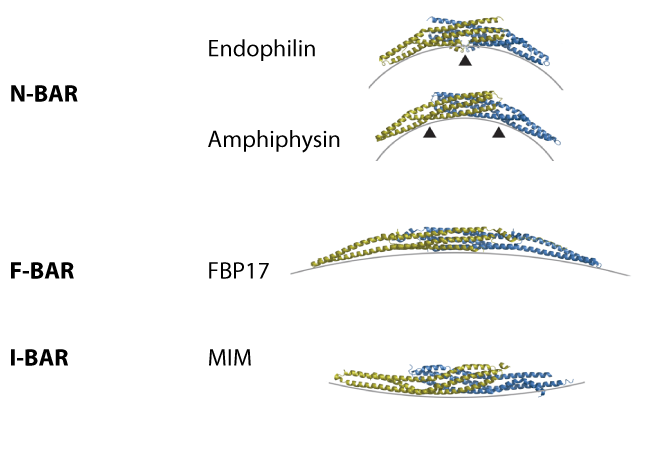
\includegraphics[scale=0.7]{figures/intro/BAR_structures}
		\caption[Structures of BAR domain dimers]{Domain structures from different families of BAR proteins. One monomer is depicted in yellow, the other in blue. Arrow heads indicate positions on the BAR domain that are inserted hydrophobically into the membrane. \textit{Adapted with persmission from John Wiley \& Sons, Inc.: The EMBO Journal (Qualmann, Koch, and Kessels, 2011), copyright (2011)}
		\label{bar_structures}}
\end{figure}

\newpage
\vspace{5mm}
BAR dimers are able to oligomerize and scaffold large areas of membrane. These scaffolds can tubulate and generate curvature across membrane regions much larger than the dimensions of a BAR dimer (Farsad et al., 2001; Peter et al., 2004) (Fig.\ref{intro_barscaffold}). BAR scaffolds can also bind membranes in a curvature-dependent manner. Correlation between the membrane shapes that they bind \textit{in vivo} and their intrinsic curvature has been shown for many BAR proteins. At membranes, they are thought to induce, stabilize, or generate specific curvature. 
	
\begin{figure}[H]
	\centering
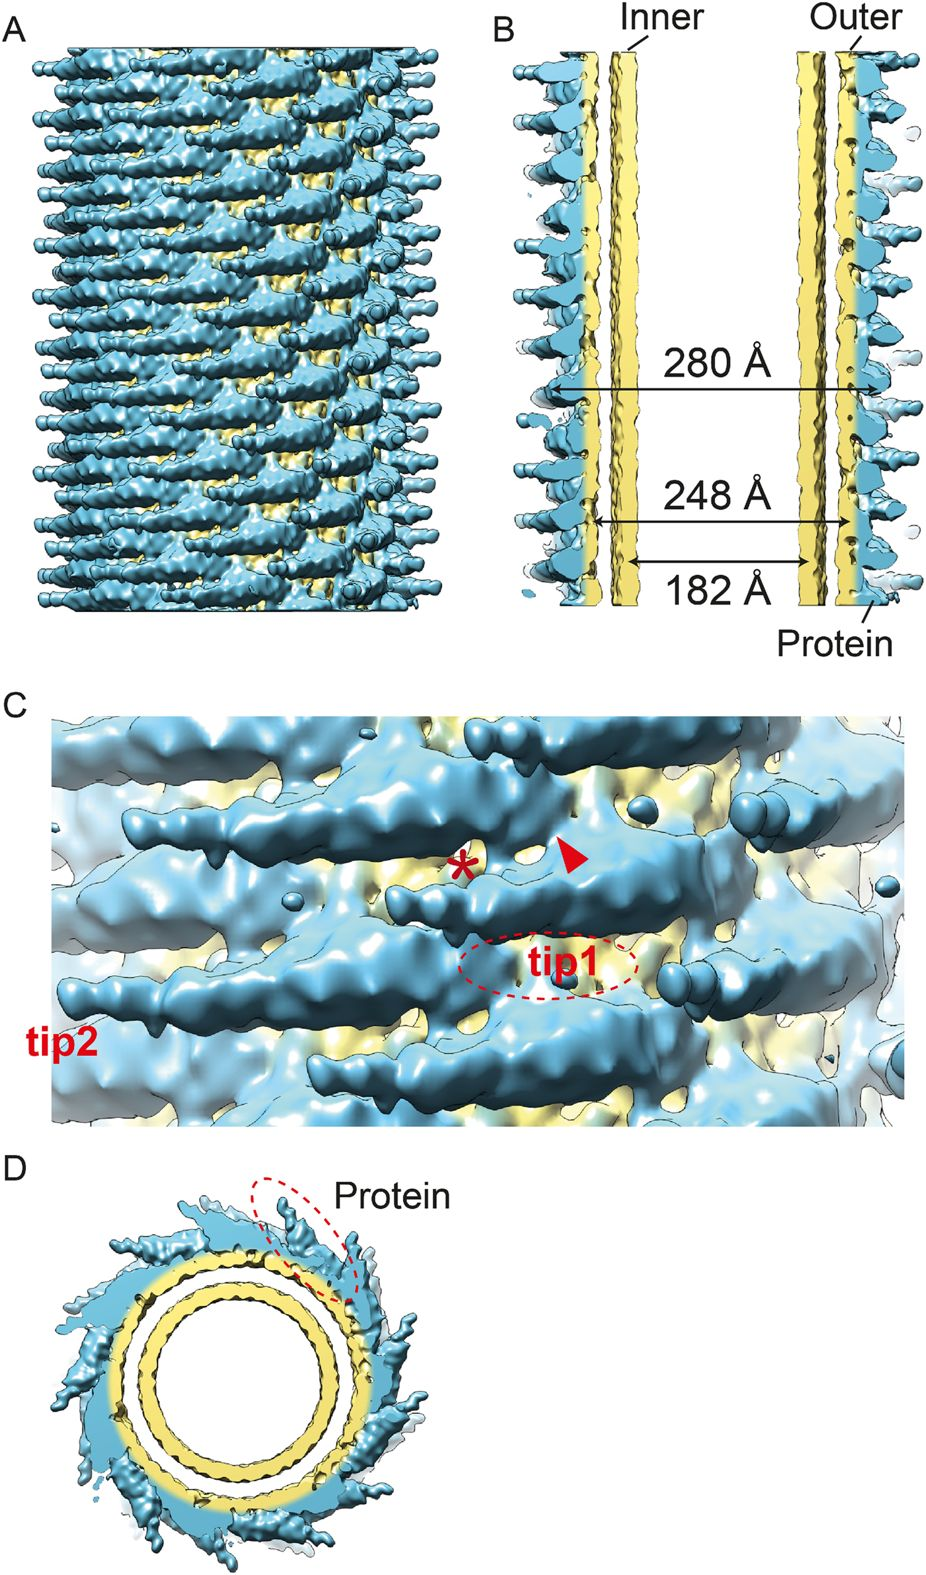
\includegraphics[scale=0.36]{figures/intro/BAR_scaffold}
\caption[BAR domain scaffolds]
{A: 3D reconstruction of amphiphysin-mediated tube from cryo-EM. Protein densities in blue, lipid densities in yellow. B: Inner and outer leaflet of membrane is indicated. Numbers correspond to total diameter, and diameter of inner and outer membrane tubes. \textit{Figure reprinted from (Adam et al., 2015) under creative commons licence \href{https://creativecommons.org/licenses/by/4.0/}{CC BY 4.0}}
\label{intro_barscaffold}}
	\end{figure}



	\subsection{NBAR proteins and membrane shapes}	
Classical BAR domain proteins form a crescent-shaped structure. Some of them have an N-terminal amphiphatic helix (N-helix), forming a subclass of classical BAR called N-BAR domains. Two significant endocytic BAR proteins, Endophilins and Amphiphysins, are both N-BAR proteins. 35-40 residues at the N-terminal region of the genes form the N-helix that acts as an amphiphatic wedge (Peter et al., 2004) . This wedge is unstructured until it is inserted into the membrane (Jennifer L Gallop, 2006). Insertion of the wedge into the one leaflet of a membrane bilayer causes displacement of lipids. This results in a change in the area of one lipid layer compared to the other, which in turn results in bending of the membrane. This indicates that N-helix insertion into a membrane bilayer could favour bending and scission (Kozlovsky and Kozlov, 2003; Boucrot et al., 2012). BAR domains lacking this helix are not able to efficiently tubulate  liposomes (Jennifer L Gallop, 2006). The N-helix also increases efficiency of binding to liposomes (Farsad et al., 2001) in a curvature sensitive manner, suggesting that the N-helix likely interacts with membrane curvatures additionally to the BAR mechanism. 


	\vspace{5mm}
High resolution structural data has shown that N-BAR proteins can form helical scaffolds on tubular membranes (Peter et al., 2004; Shimada et al., 2007; Mim et al., 2012). An energetically favourable arrangement of BAR domains consists of dimers parallel to each other, apposed to the membrane. This scaffold favours membrane tubulation and prevents scission by stabilizing the membrane tube (Boucrot et al., 2012). N-helices appear to favour vesicle formation. N-helices combined with BAR scaffolds can therefore allow coexistence of both vesicles and tubules, with preference for one or the other depending on the ratio between number of N-helices that favour vesiculation, and BAR generated scaffold stability (Boucrot et al., 2012). 



	\vspace{5mm}
BAR proteins implicated in CME , Amphiphysin and Endophilin can tubulate membranes \textit{in vitro}(Peter et al., 2004; Jennifer L Gallop, 2006; Mim et al., 2012) and form a helical scaffolds via lateral interactions between BAR dimers (Sorre et al., 2012). 



	\subsection{N-BAR protein Amphiphysin }		
%		\subsubsection{Classical BAR domains : Amphiphysin}
Two mammalian isoforms of Amphiphysins (Amph) exist. AmphI is enriched in neurons in mammals, while AmphII (Bin1) is expressed in other tissue types, with one isoform enriched in muscle T-tubule junctions (Lee et al., 2002). The only Amphiphysin in flies (d-Amph) is expressed in various tissues, and enriched at muscle T-tubule junctions. The d-Amph dimer forms a coiled coil, with each BAR domain made of three long, kinked alpha-helices (Peter et al., 2004). In-vitro, liposome tubulation activity of Amphiphysin is concentration dependent. At very high concentrations, Amphiphysin is also able to sever tubular membrane to form vesicles (Peter et al., 2004). 

	\vspace{5mm}
Amph I and II both have BAR domains, a proline rich region, and C-terminal SH3 domain.
Amphiphysin I binds clathrin and its clathrin adaptor AP2 (Razzaq et al., 2001) and can polymerize clathrin into invaginated lattices in a BAR domain dependent manner (Peter et al., 2004). Both AmphI and AmphII also bind dynamin, and the lipid phosphatase Synaptojanin (Cestra et al., 1999).




	\subsection{N-BAR protein Endophilin }	
%		\subsubsection{Classical BAR domains : Endophilin}
The Endophilin A1-A3 (EndoA) family of genes were discovered in a screen for SH3 domain containing proteins (Giachino et al., 1997). EndophilinA were subsequently found to co-localize with dynamin, interact with Synaptojanin (Ringstad, Nemoto and De Camilli, 1997) and amphiphysin (Micheva et al., 1997): all three already identified as important regulators of synaptic vesicle recycling by endocytosis. A second mammalian protein was later discovered as related to endophilin, and termed EndophilinB (EndoB). 

	\vspace{5mm}
EndoA1 isoform is found in neurons, EndoA2 is expressed ubiquitously, and EndoA3 is enriched in the brain and testes. All three are found at presynaptic membranes. Crystal structure of EndoA1 shows the same overall structure as that of amphiphysin, with an additional amphiphatic helix similar to the N-helix, located at the centre of the crescent-shaped dimer (Weissenhorn, 2005; Jennifer L Gallop, 2006) (Fig,BARstructure). This helix is thought to insert into the membrane in the same way as the N- helix, potentially increasing membrane tubulation efficiency. EndoA1 and 2 may interact with calcium channels at synapses, and may be involved in lipid modification (Huttner and Schmidt, 2000; Gallop, Butler and McMahon, 2005), suggesting different roles for the two BAR domain proteins in membrane interaction. Endophilin interacts with dynamin, NWASP and Synaptojanin proteins via its SH3 domain (Cestra et al., 1999; Otsuki, Itoh and Takenawa, 2003; Hohendahl et al., 2017)





	\subsection{NBAR protein in yeast: the Rvs complex}		
RVS161 and RVS167 (reduced viability upon starvation) genes were discovered in a screen that tested for survival under starvation conditions (Crouzet et al., 1991). Rvs161 and Rvs167 are both N-BAR domain proteins that are thought to form obligate heterodimeric complexes (Rvs) \textit{in vivo} (Sivadon, Crouzet and Aigle, 1997; Lombardi and Riezman, 2001). There is some evidence of heterodimerization: loss of one destabilizes the other, deletion phenotypes of Rvs167 is the same as that of Rvs161, and FCCS measurements indicate that they dimerize (Lombardi and Riezman, 2001; Kaksonen, Toret and Drubin, 2005; Boeke et al., 2014). However, Rvs161 functions that do not overlap with those of Rvs167 have been reported. For instance, Rvs161 interacts with Fus2 in cell-cell fusion, while Rvs167 does not (Brizzio, Gammie and Rose, 1998). It is likely that at endocytic sites the Rvs proteins function as heterodimers, while Rvs161 also forms heterodimers with Fus2 that are involved in different processes. 

	\vspace{5mm}
Rvs161 and Rvs167 are very similar in structure at the N-terminus. Both contain N-BAR domains that are 42\% similar, 21\% identical, but are not interchangeable (Sivadon, Crouzet and Aigle, 1997). In addition to the BAR domain, Rvs167 has a Glycine-Proline-Alanine rich (GPA) region and a C-terminal SH3 region. The GPA region is thought to act as a linker with no known other function, while loss of the SH3 domain affects budding pattern and actin morphology. Most Rvs deletion phenotypes can however, be rescued by expression of the BAR domain alone ( Sivadon, Crouzet and Aigle, 1997), suggesting that the BAR domains are the main functional unit of the complex. Homology modelling has shown that the BAR domain of Rvs167 is similar to Amphiphysin and Endophilin (Fig.\ref{rvs_structure}), and is therefore also likely to function similarly to the mammalian homologues. In keeping with this theory, Rvs has been shown to tubulate liposomes \textit{in vitro} (Youn et al., 2010). 


\vspace{5mm}
\begin{figure}[H]
	\centering
	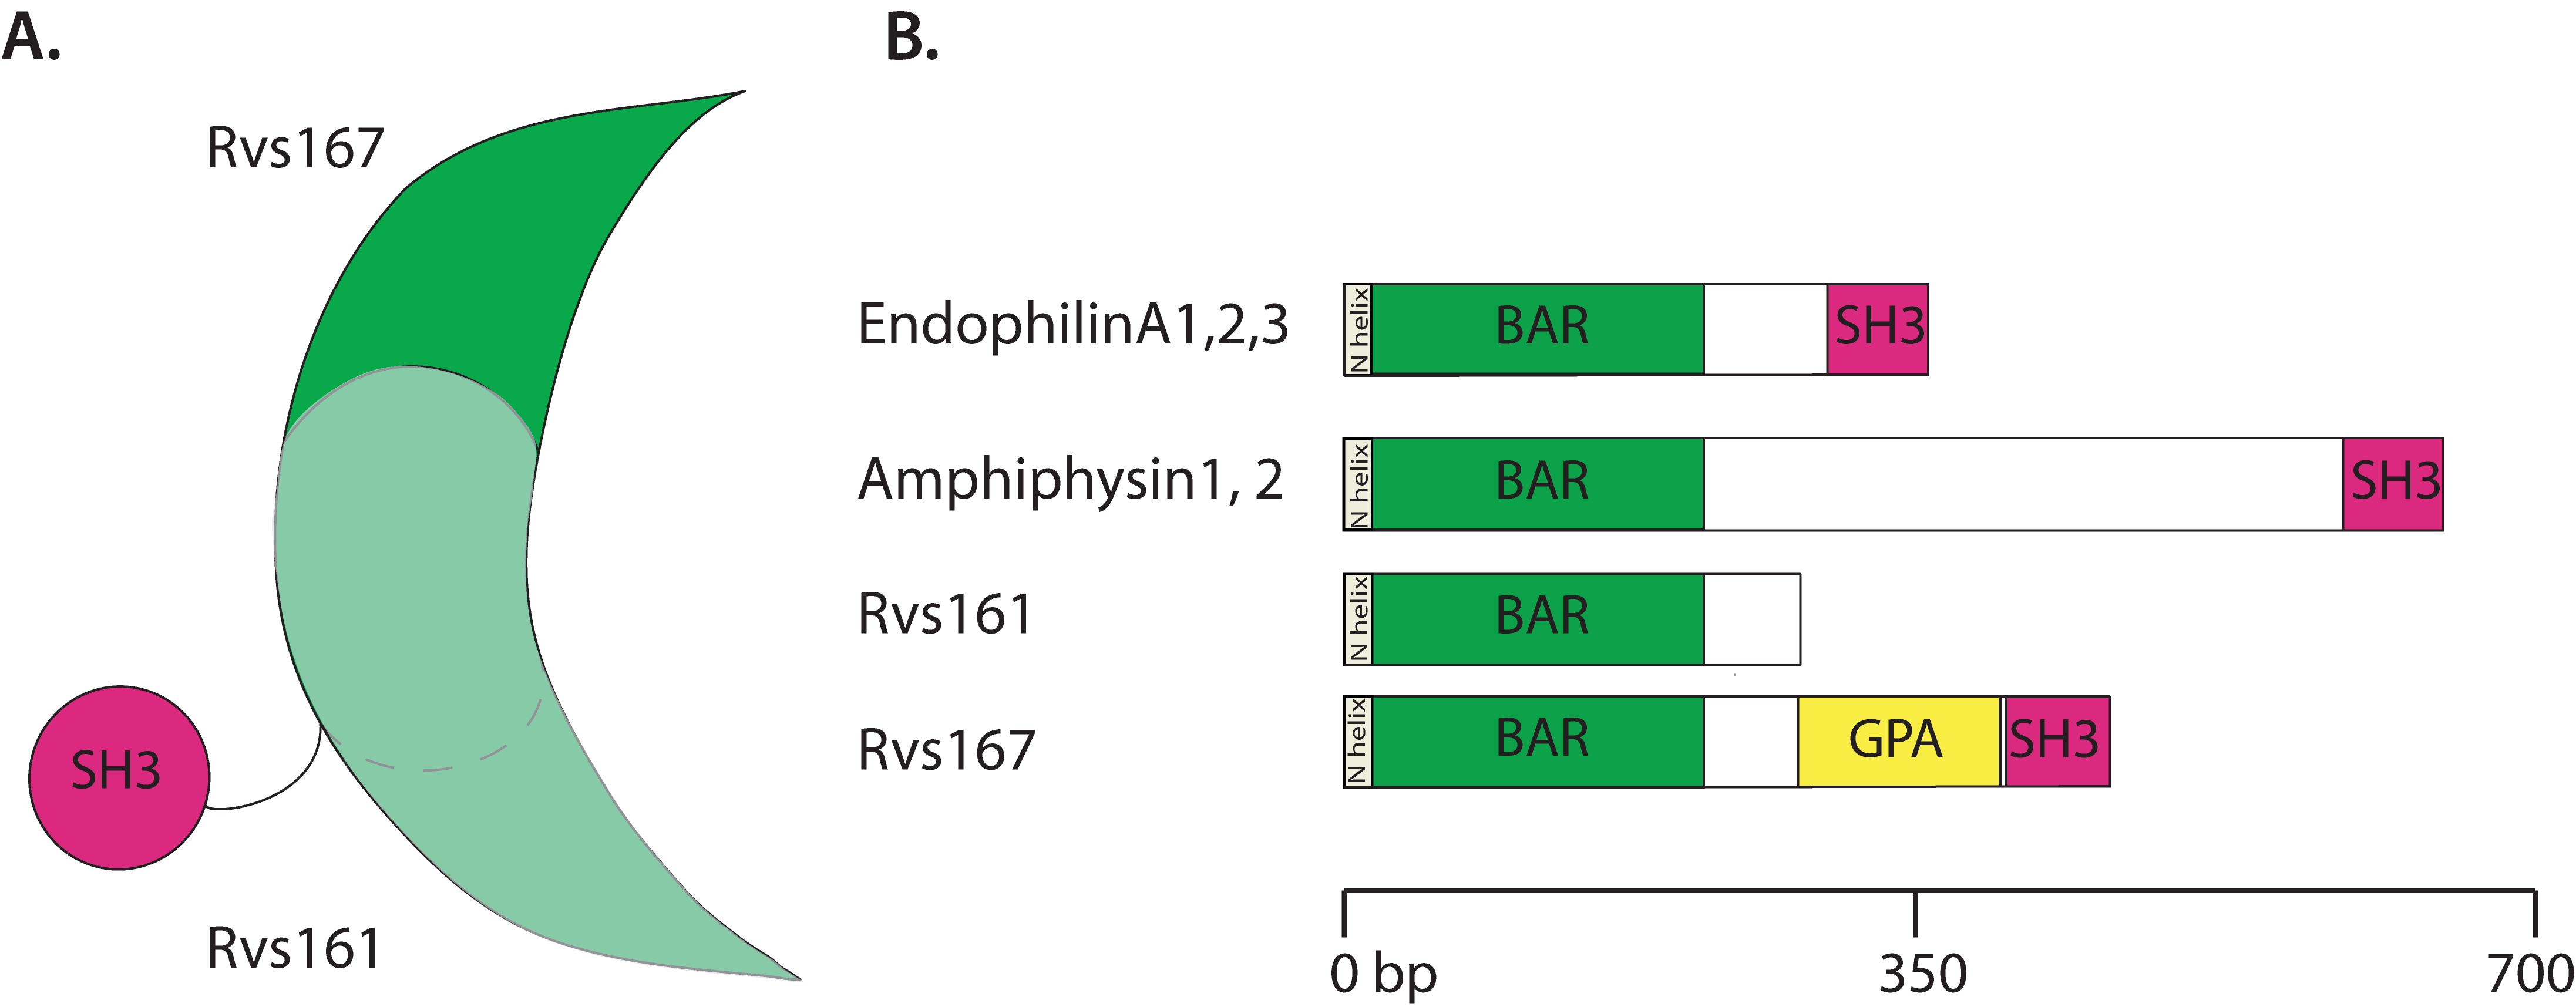
\includegraphics[scale=0.38]{figures/intro/Rvs_stucture2}
	\caption[Homolgy model of Rvs and BAR protein domains]
	{A: Schematic of Rvs dimer.	B: domain structures of endocytic BAR domain proteins
		\label{rvs_structure}}
\end{figure}


	\vspace{5mm}
\subsubsection{Rvs deletion phenotype}
Cells with Rvs deleted cannot grow under high salt conditions. They are also sensitive to increased sphingolipid levels, and have random instead of bipolar budding pattern (Bauer et al., 1993; Sivadon et al., 1995; Lombardi and Riezman, 2001; Toume and Tani, 2016). Rvs deleted cells also have aberrations in actin localization: instead of actin patches polarized to emerging buds, patches are homogenously distributed across mother and daughter cells. Loss of Rvs therefore affects localization of actin, and heightens sensitivity of yeast cells to stressful growth conditions.
 	
 	\vspace{2mm}
Rvs arrives at endocytic sites has shown that Rvs arrives in the last stage of endocytosis (Kaksonen, Toret and Drubin, 2005; Picco et al., 2015). When maximum number of Rvs is recruited, that is, at peak fluorescent intensity, movement of the Rvs complex shows a jump inwards into the cytoplasm, concomitant with a sharp decay in its fluorescent intensity, a behaviour unique among endocytic proteins (Kaksonen, Toret and Drubin, 2005; Picco et al., 2015). As mentioned earlier, loss of Rvs also affects membrane scission efficiency and causes formation of smaller vesicles than in wild-type (WT) cells. How the Rvs complex affects membrane scission, and what eventually causes membrane scission are the major questions addressed in this work




		

%(Adam et al., 2015) under creative commons licence \href{https://creativecommons.org/licenses/by/4.0/}{CC BY 4.0}}}
%\begin{itemize}
%	\item Is localization microscopy suitable to study endocytosis in budding yeast?
%\end{itemize}
 
% Chapter Template

\chapter{Aims of the study} % Main chapter title

\label{Ch:Aims} % Change X to a consecutive number; for referencing this chapter elsewhere, use \ref{ChapterX}

More than 50 different proteins are involved in clathrin-mediated endocytosis. At endocytic sites, they assemble into a small, complex and dynamic macromolecular machinery. Although individual components have been identified and well-characterized during decades of research, their structural organization is poorly understood. In my PhD project, I proposed that single-molecule localization based superresolution microscopy provides both the molecular specificity and necessary spatial resolution to study how proteins are arranged \textit{in situ} within the endocytic machinery. More specifically, I addressed the following questions:

\begin{itemize}
	\item How is Rvs recruited to endocytic sites? 
\end{itemize}

The recently developed technique of localization microscopy critically depends on dense and specific fluorescent labeling of the cellular structure of interest with a dye suitable for localization microscopy. In the first part of my project, I established an optimized sample preparation pipeline to enable high quality dual-color localization microscopy of yeast cells. These efforts are described in section \ref{LocMic_yeast}.

\begin{itemize}
	\item How does it regulate scission 
\end{itemize}
\chapter{Results}    \label{results}
\section{Recruitment of Rvs to endocytic sites}

Rvs localization in yeast endocytosis
As has been shown before, Rvs localizes to endocytic patches at the yeast plasma membrane in the late scission-stage8,9. When imaged and tracked at the equatorial plane, the late-stage coat protein Sla1 arrives and accumulates at endocytic sites, starts to moves into the cytoplasm concomitant with the arrival of actin8,9. Sla1 is pulled inwards along with the membrane and follows its movement through endocytosis. It will be used throughout this work as the marker for coat movement. As inward movement of the coat begins, the Sla1 patch is disassembled, inferred from the decay of the fluorescent intensity of Sla1-GFP8. Rvs167 arrives after a parallel membrane tube is formed, and scission occurs at 60\% of its lifetime at the plasma membrane9,10. At the time of scission, the Rvs167-GFP centroid shows a sharp jump into the cytoplasm, a profile that is unique among endocytic proteins. Concomitantly, fluorescent intensity of Rvs167-GFP shows a sudden decay.

\begin{figure}
	\centering
	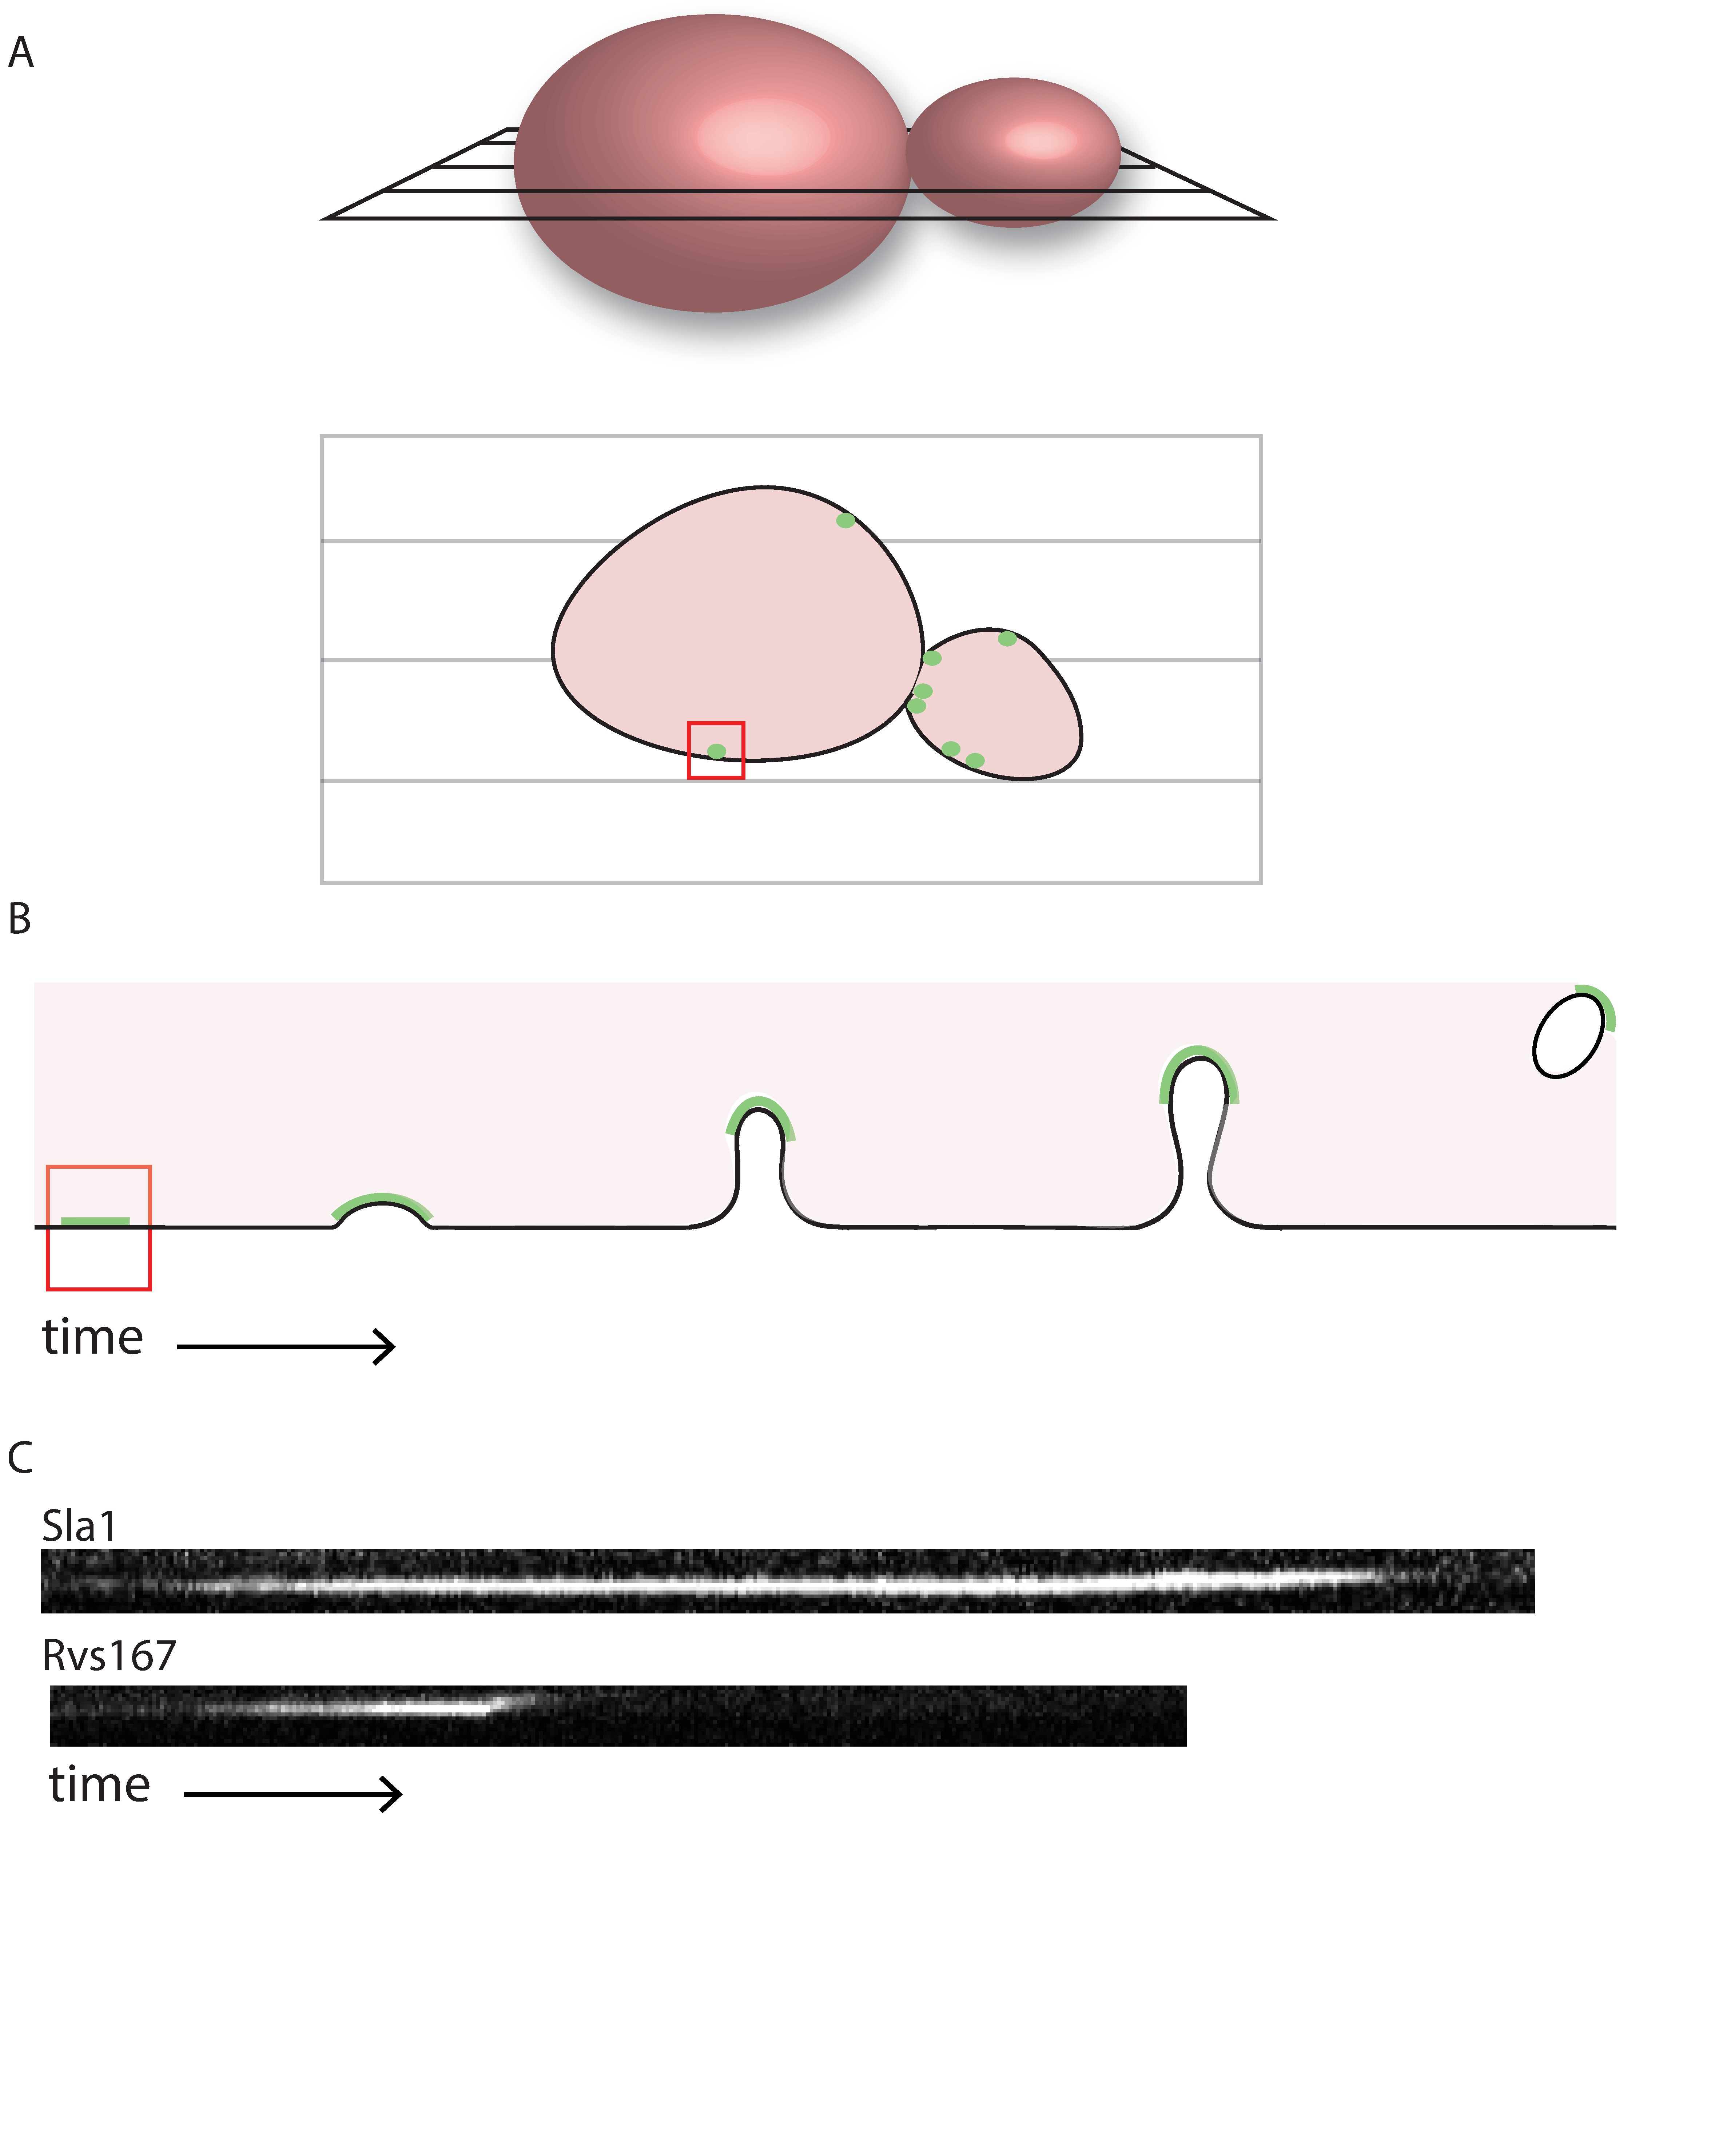
\includegraphics[width=18cm,height=18cm,keepaspectratio, valign=t]{figures/results_final/yeast_schemat_fig1_C}
	\caption[Centroid tracking yeast endocytic proteins]
	{A: Above: Schematic of a yeast cell, showing the equatorial plane. Below: Cross section of the cell at the equatorial plane, with fluorescently tagged endocytic proteins at the plasma membrane. B: Movement of coat protein Sla1-GFP shows slow inward movement, while Rvs167-GFP shows a sharp jump into the cytoplasm that is concomitant with membrane scission and vesicle formation.
2.1C: Schematic of the timeline of membrane invagionation during endocytosis, with Sla1 and Rvs167 indicated. 2.1D: Averaged centroids of Sla1 and Rvs167 through the endocytic timeline. Sla1 follows the membrane as it is pulled inwards into the cytoplasm. Rvs arrives at membrane tubes, potentially forming a scaffold around the tube. Upon membrane scission, the scaffold along the tube is disassembled, resulting in an inward jump of the Rvs167 centroid (to protein localized at the base of the newly formed vesicle), and a sharp decay in its fluorescent intensity. 
 \label{fig1_schematic}}
\end{figure}

subsection{Recruitment of Rvs and function of domains: } 

	\subparagraph{Curvature sensing or generation? }
	\mbox{}\\
Cellular membrane shape is a result of properties like rigidity, tension, intracellular pressure, that are all influenced by membrane lipid composition and the proteins embedded in it1,2. Since tension, pressure, and rigidity all oppose membrane deformation, energy is required to deform and bend it. BAR domains can generate curvature if the energy required to deform the membrane is less than the energy spent in binding flat membrane.

\vspace{5mm}
			
Curvature-generation by scaffolding and imposing its own shape on membranes has been extended to various types of BAR proteins, (Arkhipov et al., 2009; Frost et al., 2008; Henne et al., 2007; Itoh et al., 2005; Pykalainen et al., 2011; Saarikangas et al., 2009; Shimada et al., 2007; Yu and Schulten, 2013). In order for BAR scaffolds to impose membrane curvature, some requirement have to be met3: they have to have present a large membrane-interacting surface that can mediate membrane binding, have intrinsic curvature that can be imposed on the surface, and have a rigid structure that can overcome bending resistance of the membrane. Because of their shape (Peter 2004, Gallop 2006, Weissenhorn 2005), and their capacity to oligomerize into large assemblies on tubes (Mim 2012, Mizuno 2010, Takei 1999, Yin 2009), it has been suggested that BAR domains impose their shape on the membrane, and generate membrane curvature on cellular membranes. Further, it has been shown that the central BAR region is rigid and required for tubulation, both in-vivo and of liposomes4. The N-helix of NBAR domains can also generate curvature independently of the BAR scaffold (Varkey 2010, Westphal and Chandra 2013). In endophilin, the BAR domain is relatively far from the membrane, suggesting a mechanism dependent on the N-helix (Jao 2010). Different BAR domains thus likely employ different mechanisms to interact with the membrane for generating vesicles, and tubes (Ambroso 2014). For example, the N-helix of endophilin is necessary for liposome binding5, while that of amphiphysin is important, but not necessary6. 


\vspace{5mm}
Curved BAR proteins that can induce curvature are also able to sense curvature: in-vitro, BAR domains show a preferential-binding to vesicles based on their intrinsic curvature. Curvature-generation and sensing seem to intrinsically coupled mechanisms. That BAR domains are able to generate curvature does not imply that this is their function, at least in endocytosis: in-vivo, the significance of curvature-generation is not determined. Tracking over thirty different endocytic proteins in NIH-3TC cells (derived from mouse fibroblasts), TIRF imaging shows that Endophilin2 and Amphiphysin1 arrive late in the endocytic time-line right before scission7, suggesting they arrive when membrane tubes are already formed. 


\vspace{5mm}
In the case of Rvs, centroid tracking and averaging shows that the complex localizes to sites late in the endocytic timeline, close to scission8. CLEM studies have further shown that Rvs localizes to sites after the membrane invaginations are about 60nm deep into the cytoplasm: Rvs localizes once membrane curvature is established. Whether this localization is dependent on membrane curvature, recognized by the BAR domain has not been shown. 



	\subsection{BAR domain senses membrane curvature in-vivo}
	To test whether Rvs is recruited because of membrane curvature, I first imaged Rvs167-GFP without the BAR domain, that is Rvs167-delsh3-GFP (henceforth BAR-GFP). BAR-GFP forms cortical patches (Fig.2.2A), so BAR domain is able to localize to the plasma membrane in the absence of the SH3 domain. In a yeast strain expressing both BAR-GFP and Abp1-mCherry, BAR-GFP co-localizes with Abp1, indicating that BAR domains are recruited to endocytic patches (Fig2.2A, C). In order to test whether this localization is due of membrane curvature, I compared the dynamics of Rvs167-GFP against BAR-GFP in sla2del cells (Fig2.2D-F). Sla2 is a coat protein that acts as a linker between the membrane and the actin cytoskeleton by binding both via its N-terminal ANTH domain, and its C-terminal THATCH domain. This allows forces generated within the actin network to be transmitted to the membrane11. In sla2del cells, rather than cortical actin patches, an “uncoupling phenotype” is observed11,12. Although endocytic coats are formed, actin is polymerized continuously at these sites, the membrane is not pulled inwards, and vesicles are not formed: forces generated by the actin network are not transmitted to the membrane (Fig.2.2E).

\begin{figure}
	\centering
	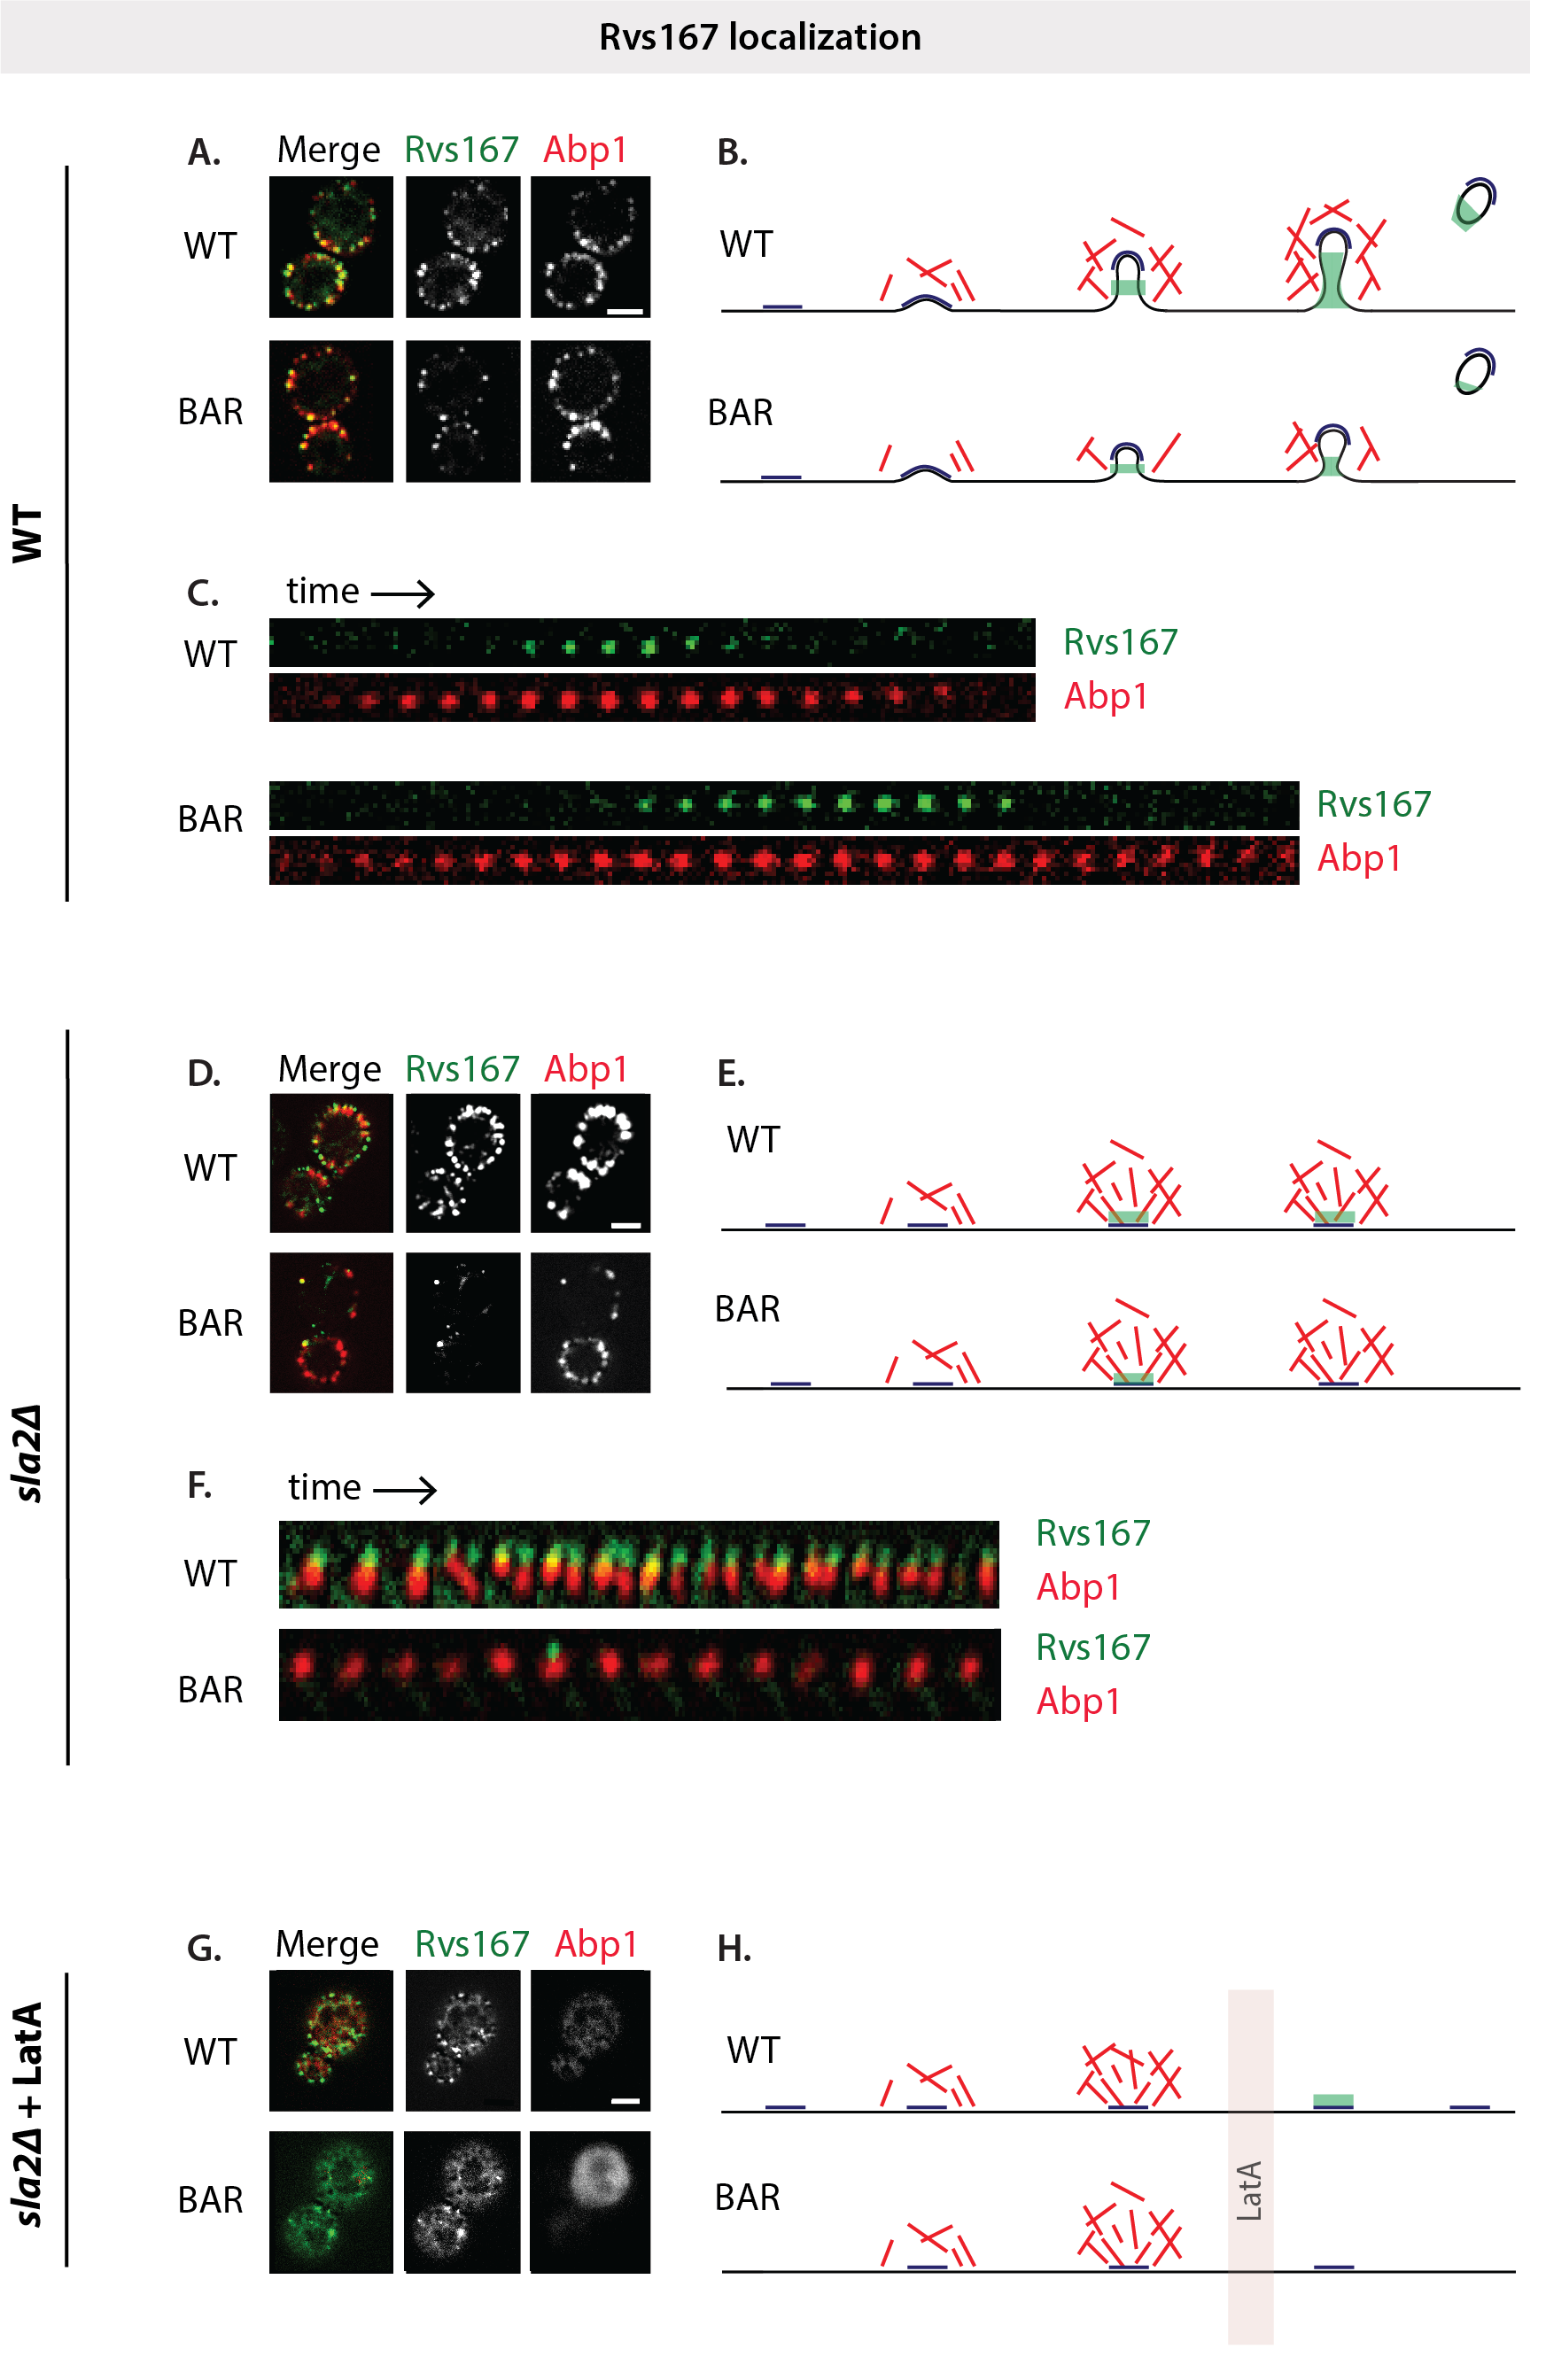
\includegraphics[width=22cm,height=22cm,keepaspectratio]{figures/results_final/sla2_del_final6}
	\caption [Localization of Rvs167 and BAR with and without membrane curvature]
	{A: Maximum intensity projections of time lapse images of Rvs167-GFP and BAR-GFP co-expressed with Abp1-mCherry. Exposure rate, 250ms for GFP and RFP channels, excited using 488 and 561nm lasers respectively. B: Schematic of membrane progression of in WT endocytic events. C: Kymograph of Rvs167-GFP and BAR-GFP localizations on the plasma membrane with Abp1-mCherry. Each frame of kymograph is every third frame from time lapse images. 
D: Maximum intensity projection of time lapse images of sla2del cells expressing Rvs167-GFP and BAR-GFP with Abp1-mCherry. E: Schematic of membrane invagination in the absence of Sla2. F: Kymograph of Rvs167-GFP BAR-GFP with Abp1-mCherry. Exposure rate 1000ms for GFP, 800ms for RFP, excited using 488 and 561nm lasers. 
G: Maximum intensity projection of time lapse images of sla2del cells expressing Rvs167-GFP and BAR-GFP, along with Abp1-mCherry, treated with LatA for 10’. Exposure rate 1000ms for GFP, 800ms for RFP. H: Schematic of membrane invagination in Sla2del cells treated with LatA. All scale bars, 2um\label{fig2_sla2del}}
\end{figure}

	\vspace{5mm}
In sla2del cells, Rvs167-GFP is recruited to the plasma membrane (Fig.2.2D,F) at the plasma membrane, and together with Abp1-mCherry. Some Rvs167-GFP patches persist at the plasma membrane, while many are assembled and disassembled at Abp1 patches. Some Rvs167 patches do not co-localize with Abp1. In sla2del cells expressing BAR-GFP, localization is mostly removed except for rare transient patches at the plasma membrane that are co-localized with Abp1, while most of the patches appear to be recruited independent of Abp1. Rvs167-GFP and BAR-GFP patches are both dynamic, indicating an interaction exists in both cases that is able to assemble and disassemble Rvs patches at the plasma membrane. 

	\subsection{The SH3 domain is able to localize Rvs in an 
		actin and \\ curvature-independent manner}

	As I show in the previous section, full-length Rvs is able to localize to cortical patches in Sla2del cells. This localization must come from the SH3 domain, since BAR alone does not localize in cells without sla2. We expected that the SH3 domain must interact with WASP or actin-binding proteins: an interaction with Abp1 has been shown, as well as with Las17, type I Myosins, and Vrp1. In order to prove this, I imaged BAR-GFP and Abp1-mCherry in sla2del cells treated with the actin sequestering agent LatrunculinA (LatA). LatA is a sea-sponge toxin that binds monomeric actin and prevents incorporation of actin into filaments. Since high actin turnover is required at endocytic sites, LatA effectively disassembles WASP components and other actin-binding proteins of the endocytic machinery, and blocks endocytosis. In combination with the sla2 deletion, latA treatment will effectively prevent membrane curvature as well as remove actin-binding proteins from endocytic sites. Loss of actin binding proteins is verified by the loss of Abp1 signal in the RFP channel.


	\vspace{5mm}
Surprisingly, full-length Rvs is transiently localized to the plasma membrane in spite of the LatA treatment, suggesting that the SH3 domain is able to recruit Rvs to the plasma membrane. This recruitment occurs in the absence of a BAR-membrane interaction, since BAR-GFP localization is completely removed in LatA treated cells. Rvs167-GFP patches are transient, so an assembly-disassembly mechanism is mediated by the SH3 domain outside of its BAR domain interaction. Localization of Rvs161, which does not have an SH3 domain, is also removed by LatA treatment12, supporting the conclusion that the BAR domains of the Rvs complex senses membrane curvature in-vivo. 

	\subsection{Loss of the SH3 domain affects endocytic progression}s
Since the SH3 domain plays a surprisingly larger role in the function of Rvs, I investigated its effect further. The SH3 domain generally mediates protein-protein interaction by binding to proline-rich sequences that contain a core PXXP motif13,14 (where X is any amino acid). These domains are ubiquitous in cellular interaction pathways, and several endocytic proteins have at least one SH3 domains, used to self-regulate activity, as well as to modulate local concentrations of protein. Although SH3 domains are abundant, they appear to have specific of binding partners. For Rvs167 SH3, neither the specific binding partner, nor its function in the scheme of endocytosis is known. From early work, the BAR domain is expected to act as the functional module of the Rvs proteins: most of the phenotypes of Rvs deletion can be compensated by expression of the BAR domain alone, although the SH3 domain is required in addition to the BAR domain for bipolar budding pattern15. 

	\vspace{5mm}
In order to probe the contribution of the Rvs SH3 domain to endocytosis, I studied coat and Rvs dynamics by expressing Rvs167 without the SH3 domain. Quantification of the number of BAR-GFP molecules reruited to endocytic sites shows that without the SH3 domain, recruitment is reduced by half (30.1 +/- 9.9 for BAR-GFP compared to 53.2 +/- 5.3 for Rvs167-GFP), although the cytoplasmic concentration of protein is not affected compared to Rvs167-GFP. The inward jump of BAR-GFP is reduced, compared to the full-length protein, and a number of BAR-GFP patches remain on the plasma membrane and are disassembled without inward movement. Movement of the coat protein Sla1 is similarly reduced. Sla1 moves in to approximately 50nm instead of the 140nm found in WT invaginations. Abp1-GFP recruitment without the SH3 domain is reduced to 50\% of WT recruitment, from 347+/- 30.6 molecules in WT to 172.6 +/- 12.9. Shorter invaginations with a maximum of 60nm have been observed in the case of Rvs167 deletion by CLEM 10, which is about the same length as those observed in the SH3 deletion: loss of the SH3 domain appears to be detrimental to the function of the Rvs complex.

\begin{figure}
	\centering
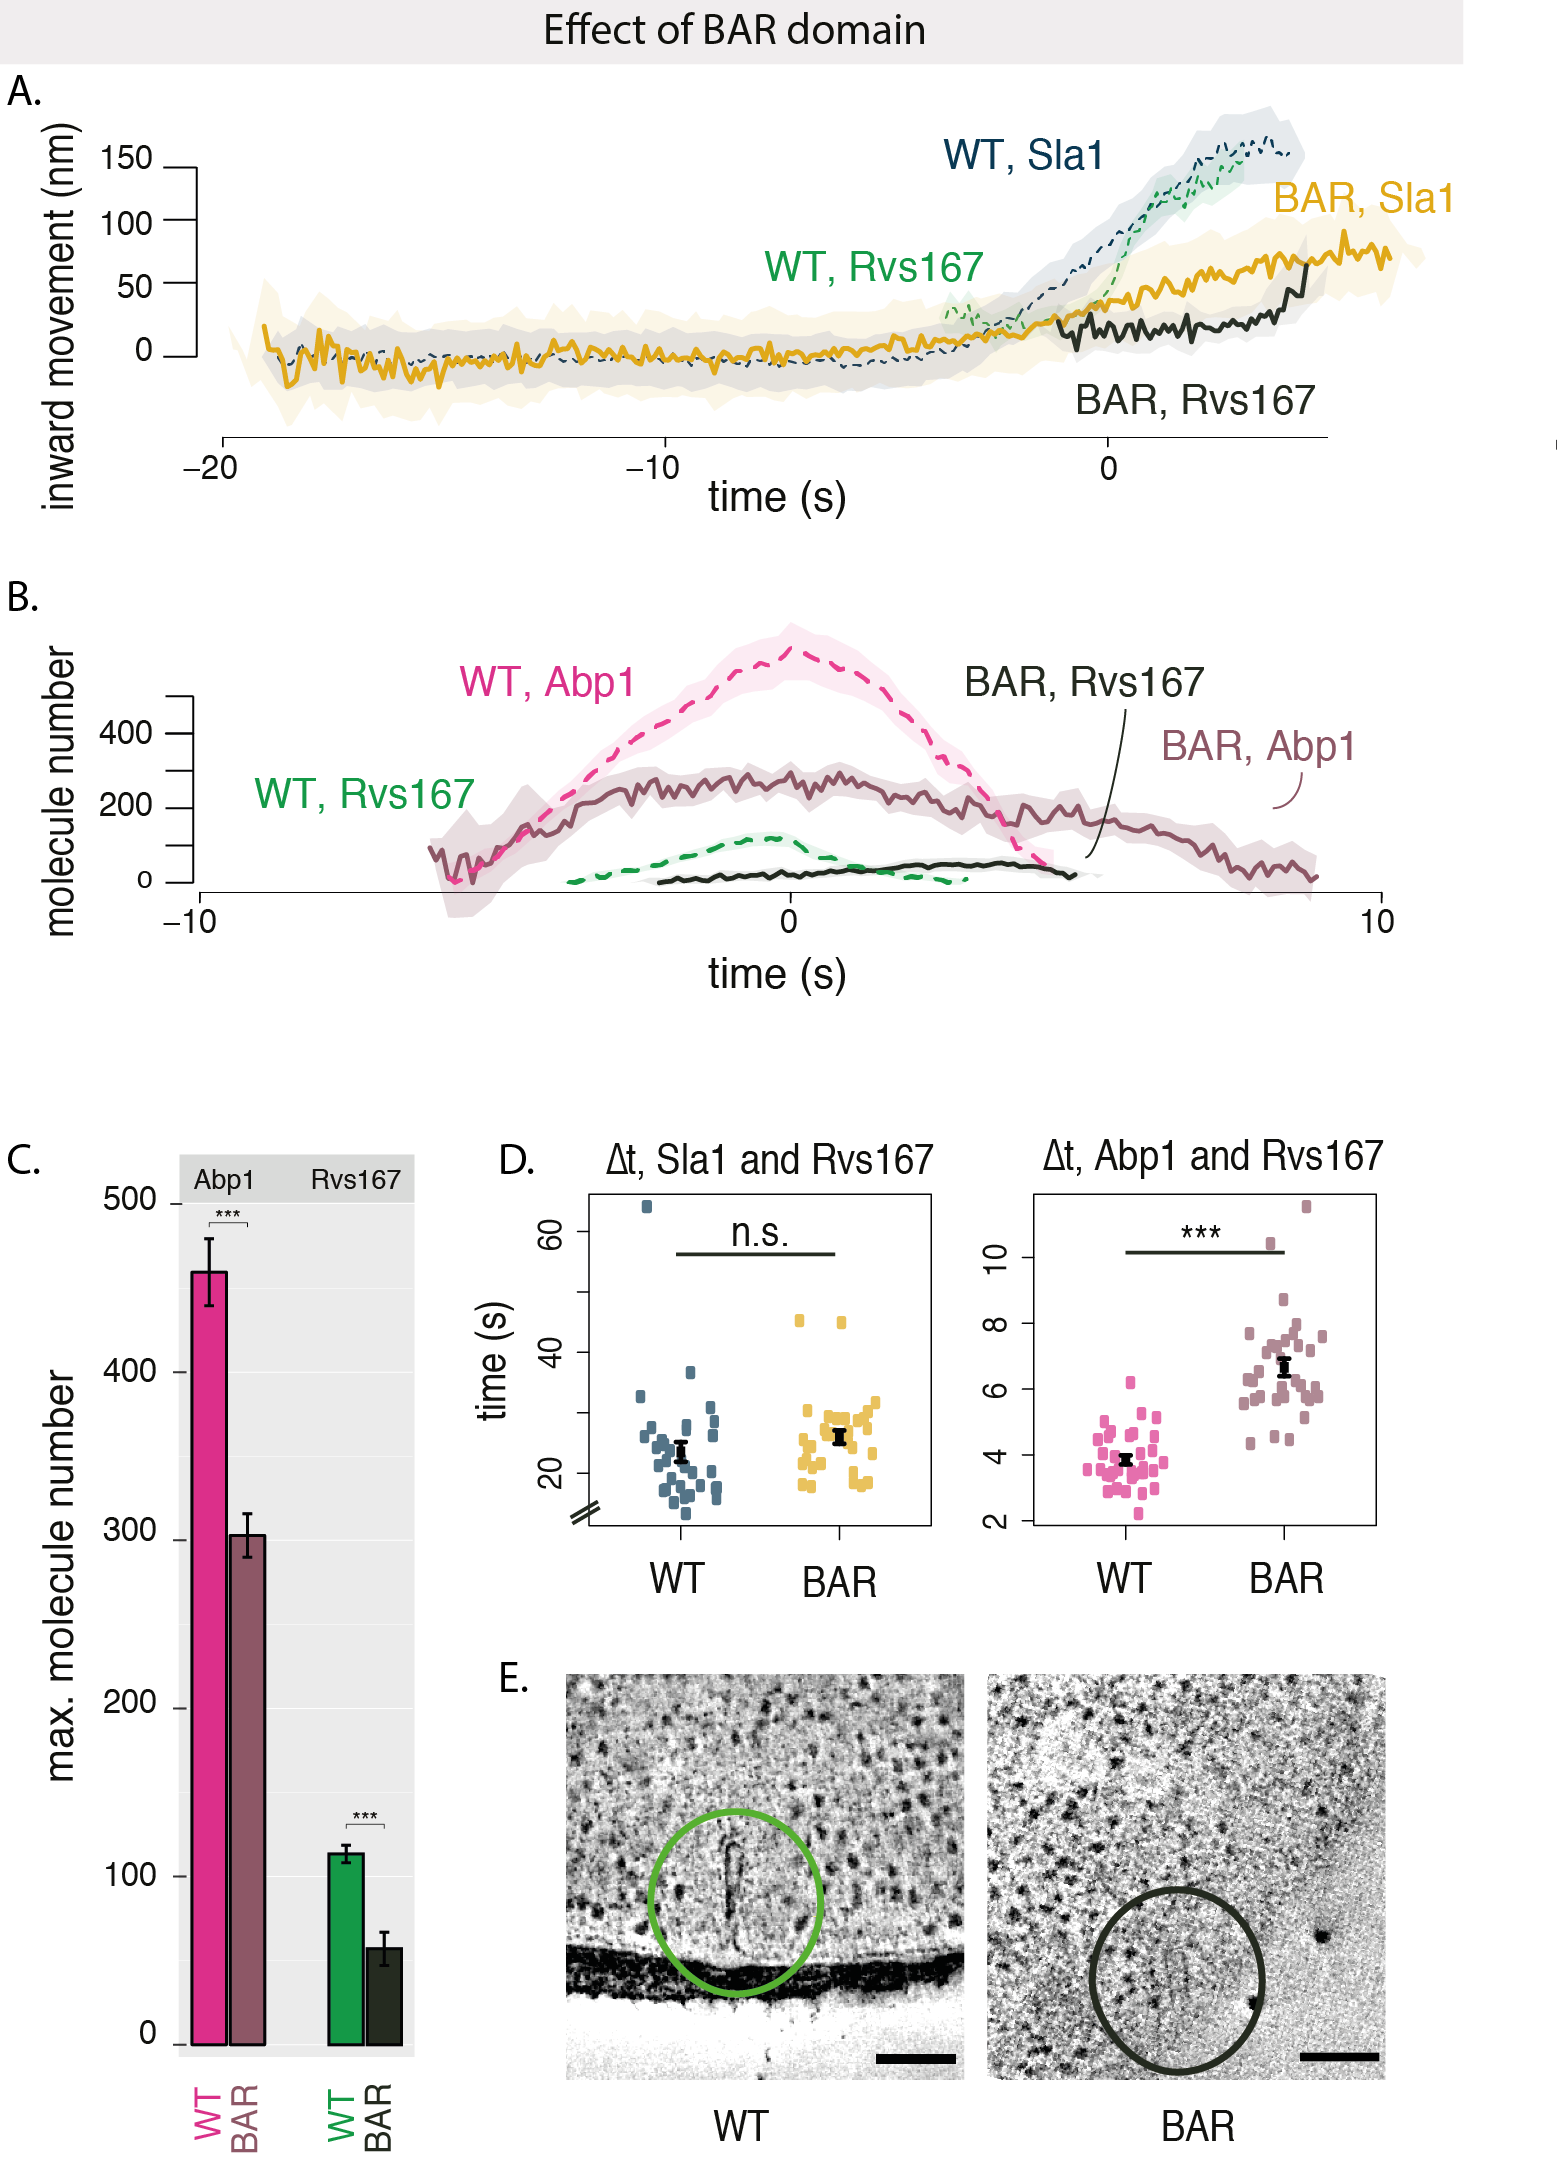
\includegraphics[width=21cm,height=21cm,keepaspectratio]{figures/results_final/delsh3_6}
	\caption [Effect of the Rvs167 SH3 deletion]
	{A: Averaged centroid movement of Sla1 and Rvs167 in WT and BAR strains. Centroids are aligned in time so that time=0 corresponds to the Abp1-mCherry fluorescent intensity peak in simultaneous dual-color imaging of the corresponding strains. Exposure rate 250ms.
B: Molecule numbers of Abp1-GFP and Rvs167-GFP and BAR-GFP with standard error of mean. 
C: Lifetimes are measured by TIRF in Rvs167-GFP/ Abp1-mCherry and Rvs167-GFP/ Sla1-mCherry strains in WT and BAR strains. Exposure 560ms for each channel. Mean and standard error of the mean are shown,  * = p $\leq$ 0.05 , ** = p$\leq$ 0.01, *** = p $\leq$ 0.001 . P values of two-sided t test. 
D: Difference in time between arrival of Sla1-mCherry and Rvs167-GFP, and Abp1-mCherry and Rvs167-GFP in WT and BAR strains. Exposure 560ms for each channel. Mean and standard error of the mean are shown, * = p$\leq$ 0.05, ** = p$\leq$ 0.01, *** = p$\leq$ 0.001. P values of two-sided t test.\label{fig2_sh3del}}
\end{figure}
	\vspace{5mm}
	
For a more detailed inquiry into changes in the endocytic machinery without the Rvs167 SH3 domain, I quantified the lifetimes of Rvs, and coat and actin network using Sla1 and Abp1 as markers in SH3 deleted cells using total internal reflection fluorescence (TIRF) microscopy. Unlike epifluorescence microscopy at the equatorial plane, that has been the method used for quantification so far, when using TIRF, only fluorophores up to a depth of about 100nm from the glass-sample interphase are excited. This reduces fluorescent signal from the cytoplasm, allowing detection of low intensity fluorescent signal, and is a better method for quantification of protein lifetime than epifluorescence microscopy. Lifetimes of BAR-GFP, Sla1-mCherry and Abp1-mCherry in SH3 deleted cells is compared against WT Rvs167-GFP, Sla1-mCherry and Abp1-mCherry. 

	
	\vspace{5mm}
While the lifetimes of Rvs167 and BAR are similar, and Sla1 lifetime with and without the SH3 domain is also similar, there is a significant increase in the lifetime of Abp1 lifetime in the absence of the SH3 domain. I then looked for differences in the sequence of recruitment of these endocytic proteins by looking at the difference in time between recruitment of Sla1 and Rvs, and the difference in time between recruitment of Abp1 and Rvs in the WT and SH3 deleted strain. The time difference between recruitment of Sla1 and full-length and SH3 deleted Rvs167 is unchanged, while the difference in time between recruitment of Abp1 and BAR is increased when compared to WT Rvs.

	\subsection{What does the SH3 domain interact with?}
		\subsubsection{Vrp1}
		\subsubsection{Type 1 myosins}
		\subsubsection{Las17}


	\subsection{Other potential mechanisms of assembly/ disassembly of Rvs}		
			\subsubsection{Interaction with Calmodulin}
			\subsubsection{FBAR protein Bzz1}
				
\section{Role of the SH3 domain}	
Is likely that SH3 domains, are involved in modulating oligomerization (5, 14) and MC-S, G (15, 82). 	
\section{Role of the N-helix}			
		
\section{Scission mechanisms}

	\subsection{Membrane scission is not dependent on Vps1}
	Yeast dynamin is the obvious solution to membrane scission. Although none of the three dynamin- like proteins has a proline-rich domain, one of the yeast dynamins, Vps1 has been suggested to be involved in endocytosis11,12. Rooij et al., suggest that Vps1 localizes to endocytic sites in the late scission stage, and that the vps1Δ rvs167Δ double mutant increases membrane retraction rates after invagination, an indication of scission failure. Vps1-GFP does not localize to endocytic sites in Gadila et at.,13, but localizes to the golgi body and to vacuoles. Kishimoto et al, do not find a colocalization between Vps1 and Abp1 localization, and also report that the vps1Δ rvs167Δ  double mutation does not affect membrane retraction rates. Vps1 tagged with both GFP as well as superfolded GFP, and imaged by TIRF microscopy fails to colocalize with Abp1 (data not shown, personal communication with Andrea Picco). The debate concerning the involvement of Vps1 in membrane scission in yeast has been compounded by the possibility that the GFP tag at the Vps1 C-terminal could interfere with its localization to endocytic sites, or its interaction with the Rvs complex. 
	
	\vspace{5mm}
	In order to exclude the possibility of interference from the GFP tag, I investigated the role of Vps1 by studying coat and scission proteins in vps1Δ cells. The late coat protein, Sla1 is used as a marker for coat movement, and Rvs167 marks scission time. Centroid tracking and averaging is performed as described in Picco et al., and inward movements of the both in wild-type and vps1Δ cells are compared. 

	\begin{figure}
	\centering
	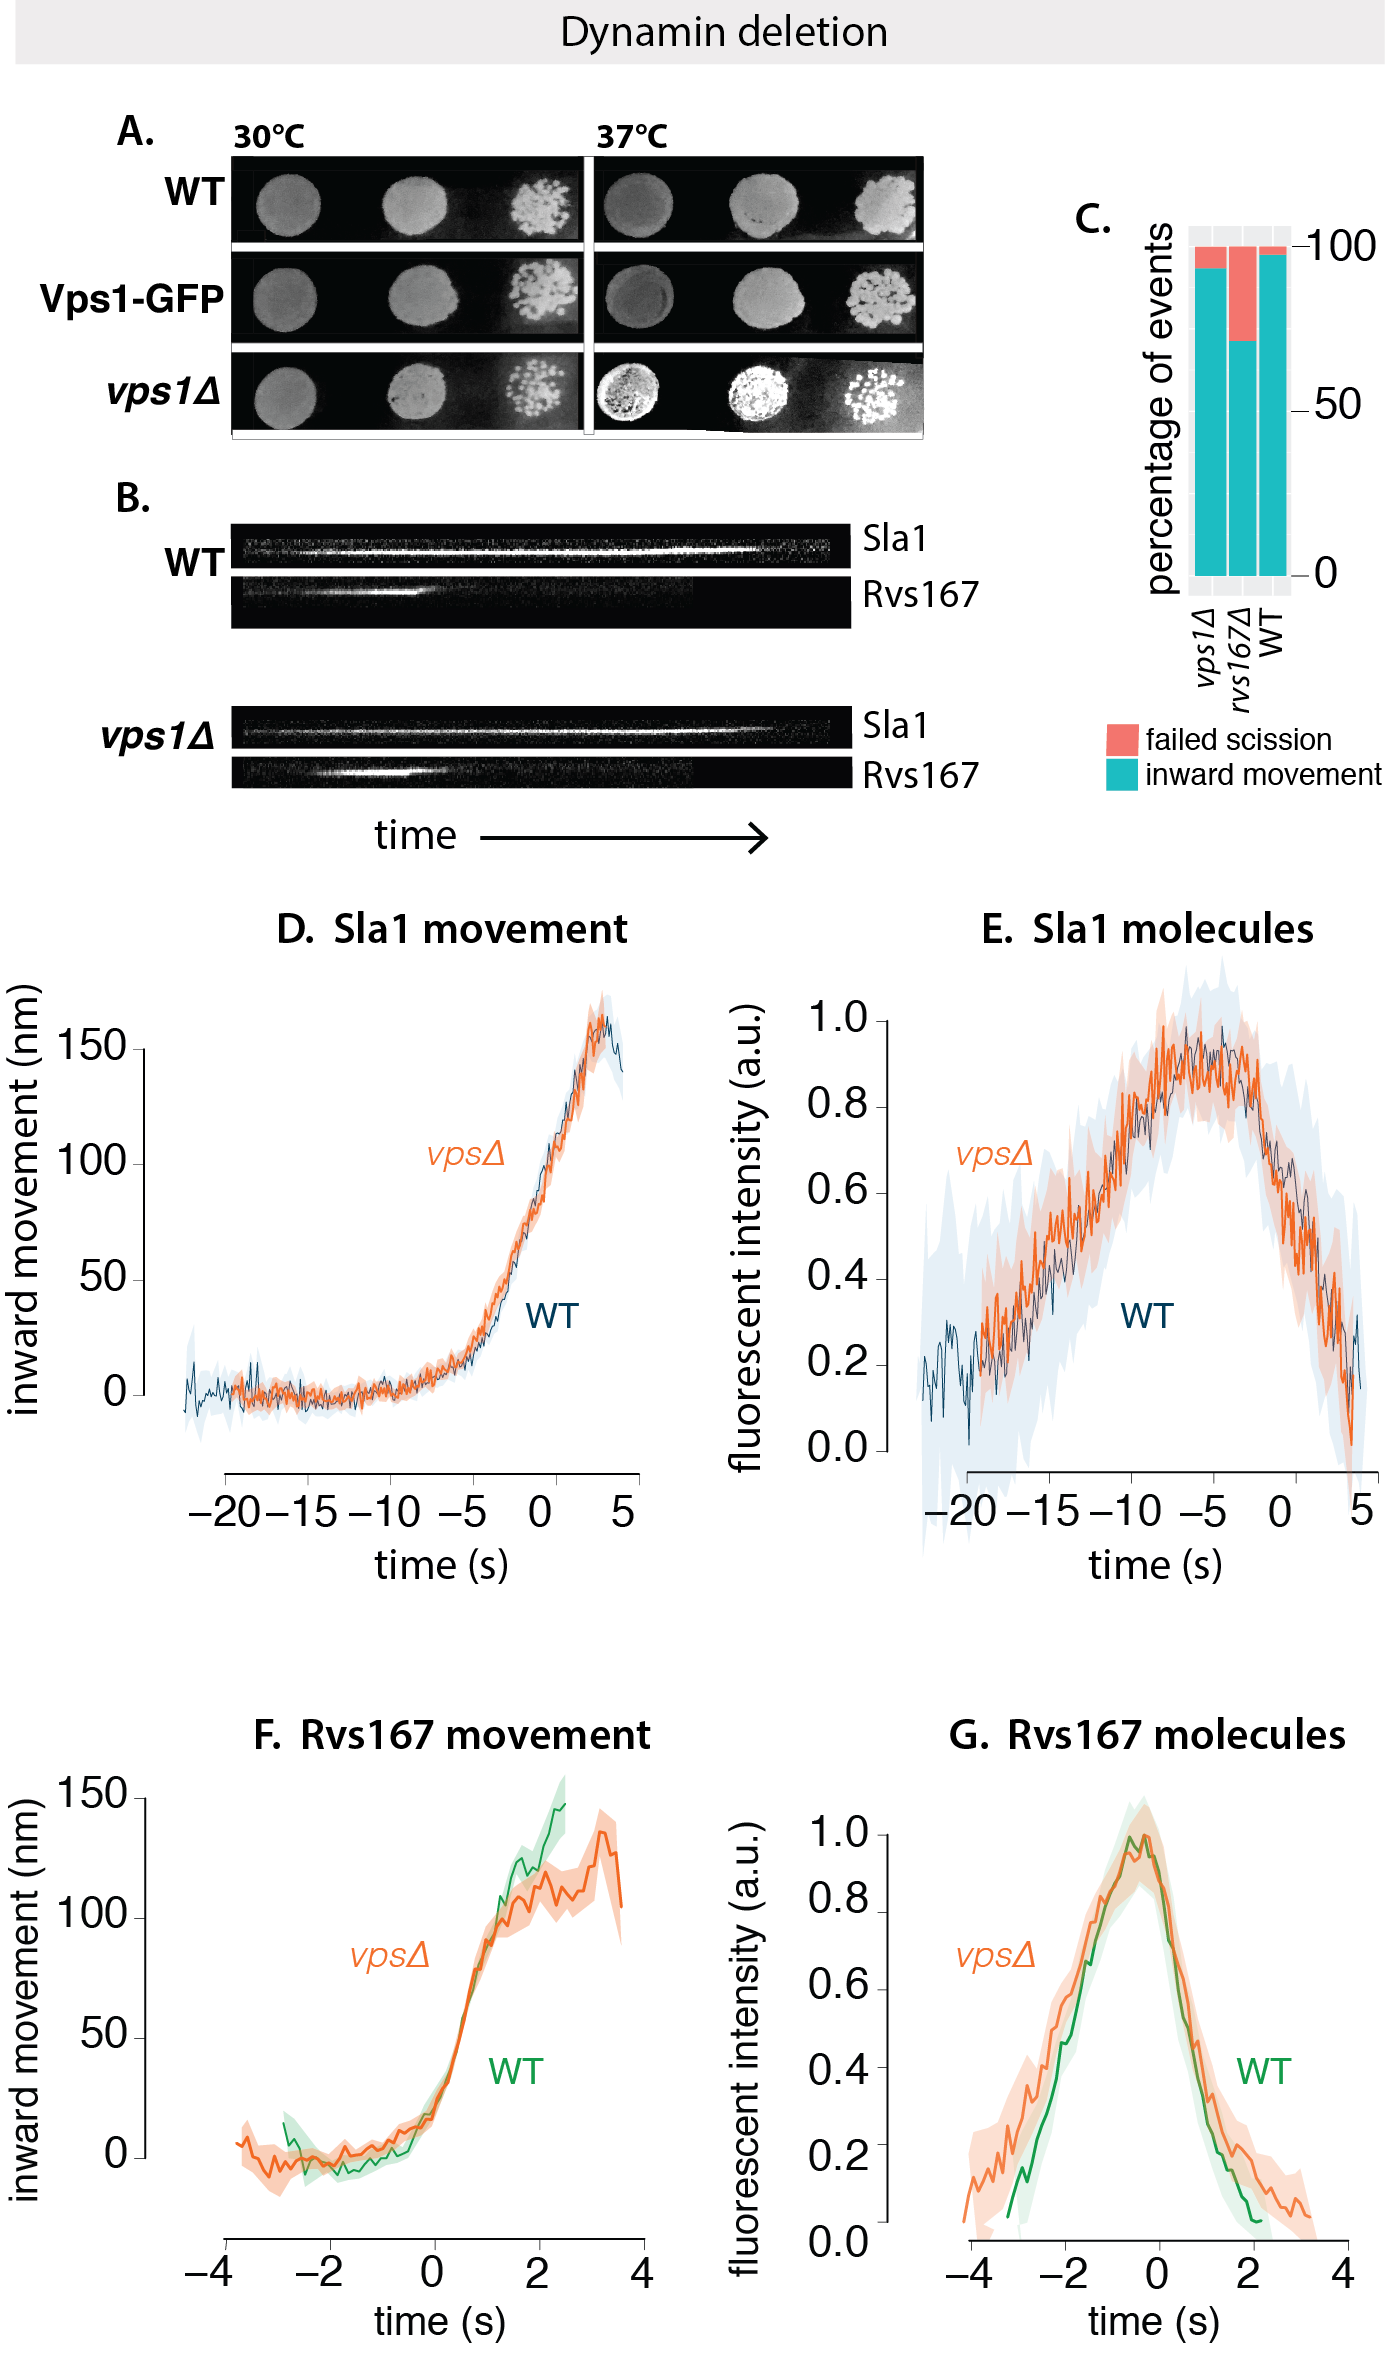
\includegraphics[width=20cm,height=20cm,keepaspectratio]{figures/results_final/vps}
	\caption{Rvs localization in vps deletion\label{fig3_vpsdel}}
	\end{figure}

	
	\vspace{5mm}
	vps1Δ cells exhibit a growth defect at 37C, as has been reported11. Sla1-GFP accumulates at the plasma membrane, moves inwards, and disassembles like in WT. The average lifetime of Sla1-GFP at endocytic patches remains unchanged. In WT cells, Sla1 moves into the cytoplasm about 140nm before membrane scission occurs. If Vps1 was required for membrane scission, Sla1 would be expected to undergo delayed or failed scission. However, vps1Δ does not increase the rate of membrane retraction. Inward movement of Sla1 is also not changed: it moves inward at the same rate, and to similar maxima of 140nm. Further, the averaged centroid of Rvs167 would not show the sharp jump into the cytoplasm if scission failed. If scission was delayed, the average lifetime of Rvs167 would increase. The inward movement of Rvs167, and its average lifetime, however, remains the same as in WT. I conclude that if Vps1 does localize to endocytic patches in S.cerevisiae, it is not involved in regulating membrane scission.  


	\subsection{Lipid hydrolysis and membrane scission}
	
	\subparagraph{Can lipid hydrolysis drive membrane scission?}
	Another hypothesis has proposed that regulated lipid hydrolysis can cause vesicle scission19. Phosphatidylinositols (PIs) and their derivatives play important roles in many cellular processes including membrane trafficking and cell signalling. Conversion between lipid types is driven by kinases, lipases, and phosphatases and controlled throughout the membrane trafficking pathway. 
	
	\vspace{5mm}
	Phosphatidylinositol(4,5)-biphosphate (PI (4,5) P2) is an important lipid type found at the cell surface, and is enriched and depleted from endocytic sites at the plasma membrane in concert with the assembly and disassembly of the endocytic machinery. Synaptojanins form a subset of inositol polyphosphate 5-phosphatases that hydrolyze PI(4,5)P2 to PI(4)P by removing the phosphate at the 5’ position of the inositol ring, and play a role in CME and intracellular signalling, as well as in modulating the actin cytoskeleton14. Synaptojanins localize to endocytic sites, and in mammalian cells, disruption of Synaptojanin genes results in cellular accumulation of PI(4,5)P2 and coated vesicles at the plasma membrane, suggesting a role for lipid hydrolysis in releasing coat proteins from nascent vesicles. Syaptojanins contain an N-terminal homology domain with the cytoplasmic domain of the yeast SAC1 gene, that is implicated in lipid metabolism, actin morphology, and vesicle transport in the secretary pathway15. A central catalytic domain is followed by a proline-rich C-terminal regions that are the canonical interaction partners of SH3 domains: they are known to interact with actin binding proteins and BAR domain proteins, potentiating also a role in membrane invagination and scission. 
		
	\vspace{5mm}
	The yeast encodes three Synaptojanin-like proteins- Inp51, Inp52 and Inp53- that regulate phospholipid metabolism. Double deletion of Inp51 and Inp52 has been shown to increase the lifetime of endocytic proteins and produce aberrant membrane invaginations that could indicate scission failure and defective endocytosis, although uptake of extracellular membrane appears to proceed in spite of the morphological aberrations16,17. Deletion of Inp52 along with Rvs167 increases scission failure rate, supporting a possible role in membrane scission18. Loss of inp51 mutation shows a increase in bulk PIP2 level, although chages in PIP2 levels have not been reported for mutations of inp52, and are not measured locally at the endocytic sites19,20.

	\subparagraph{Loss of yeast synaptojanins does not significantly affect coat and Rvs dynamics}
	\mbox{}\\
	In a model proposed by Liu et al, Synpatojanins and BAR proteins interact to regulate PI(4,5)P2 hydrolysis, which in turn drives membrane scission. Here, the Rvs scaffold on the membrane tube protects the underlying PIP2 from hydrolysis. Synaptojanin arrives at sites, and hydrolyses unprotected PIP2. This generates a boundary between BAR-protected PIP2 at the tube and PIP at the bud tip. The lipid boundary produces a line tension at the interphase that would generate enough force to pinch off a vesicle. 
	
		\begin{figure}
		\centering
		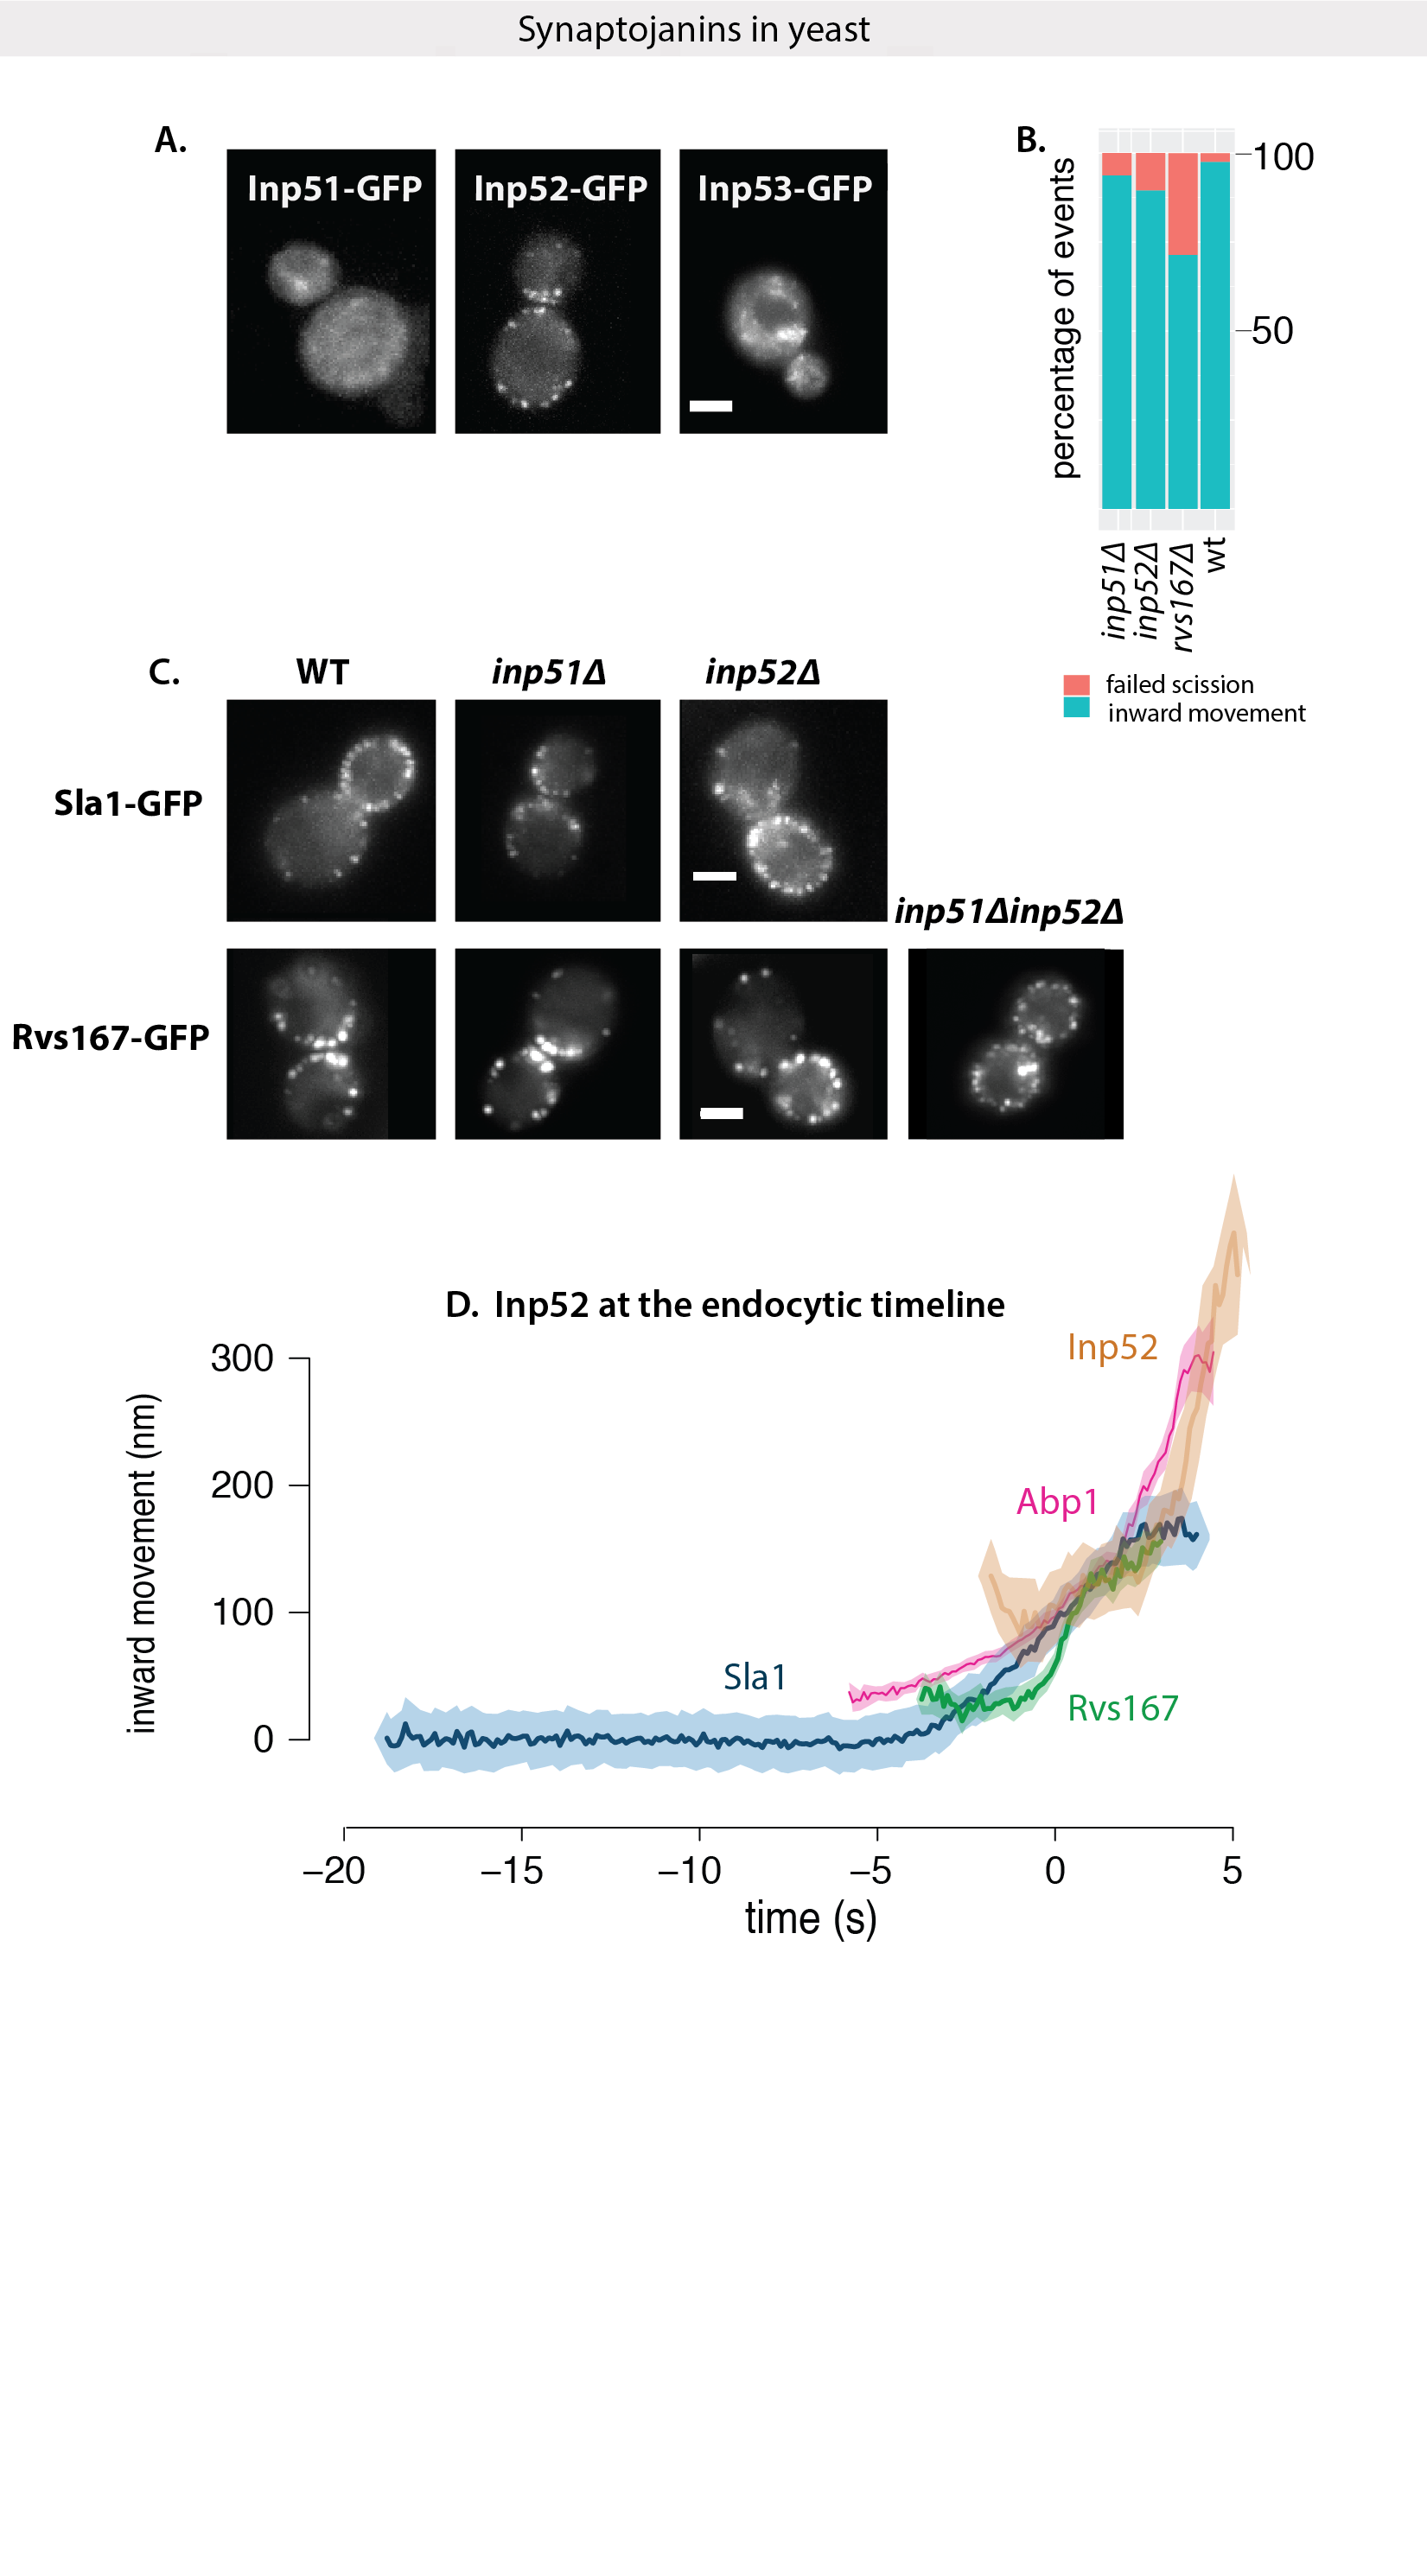
\includegraphics[width=22cm,height=22cm,keepaspectratio]{figures/results_final/inp}
		\caption{Yeast synaptojanins \label{fig4_inp}}
		\end{figure}
		
		\begin{figure}
		\centering
		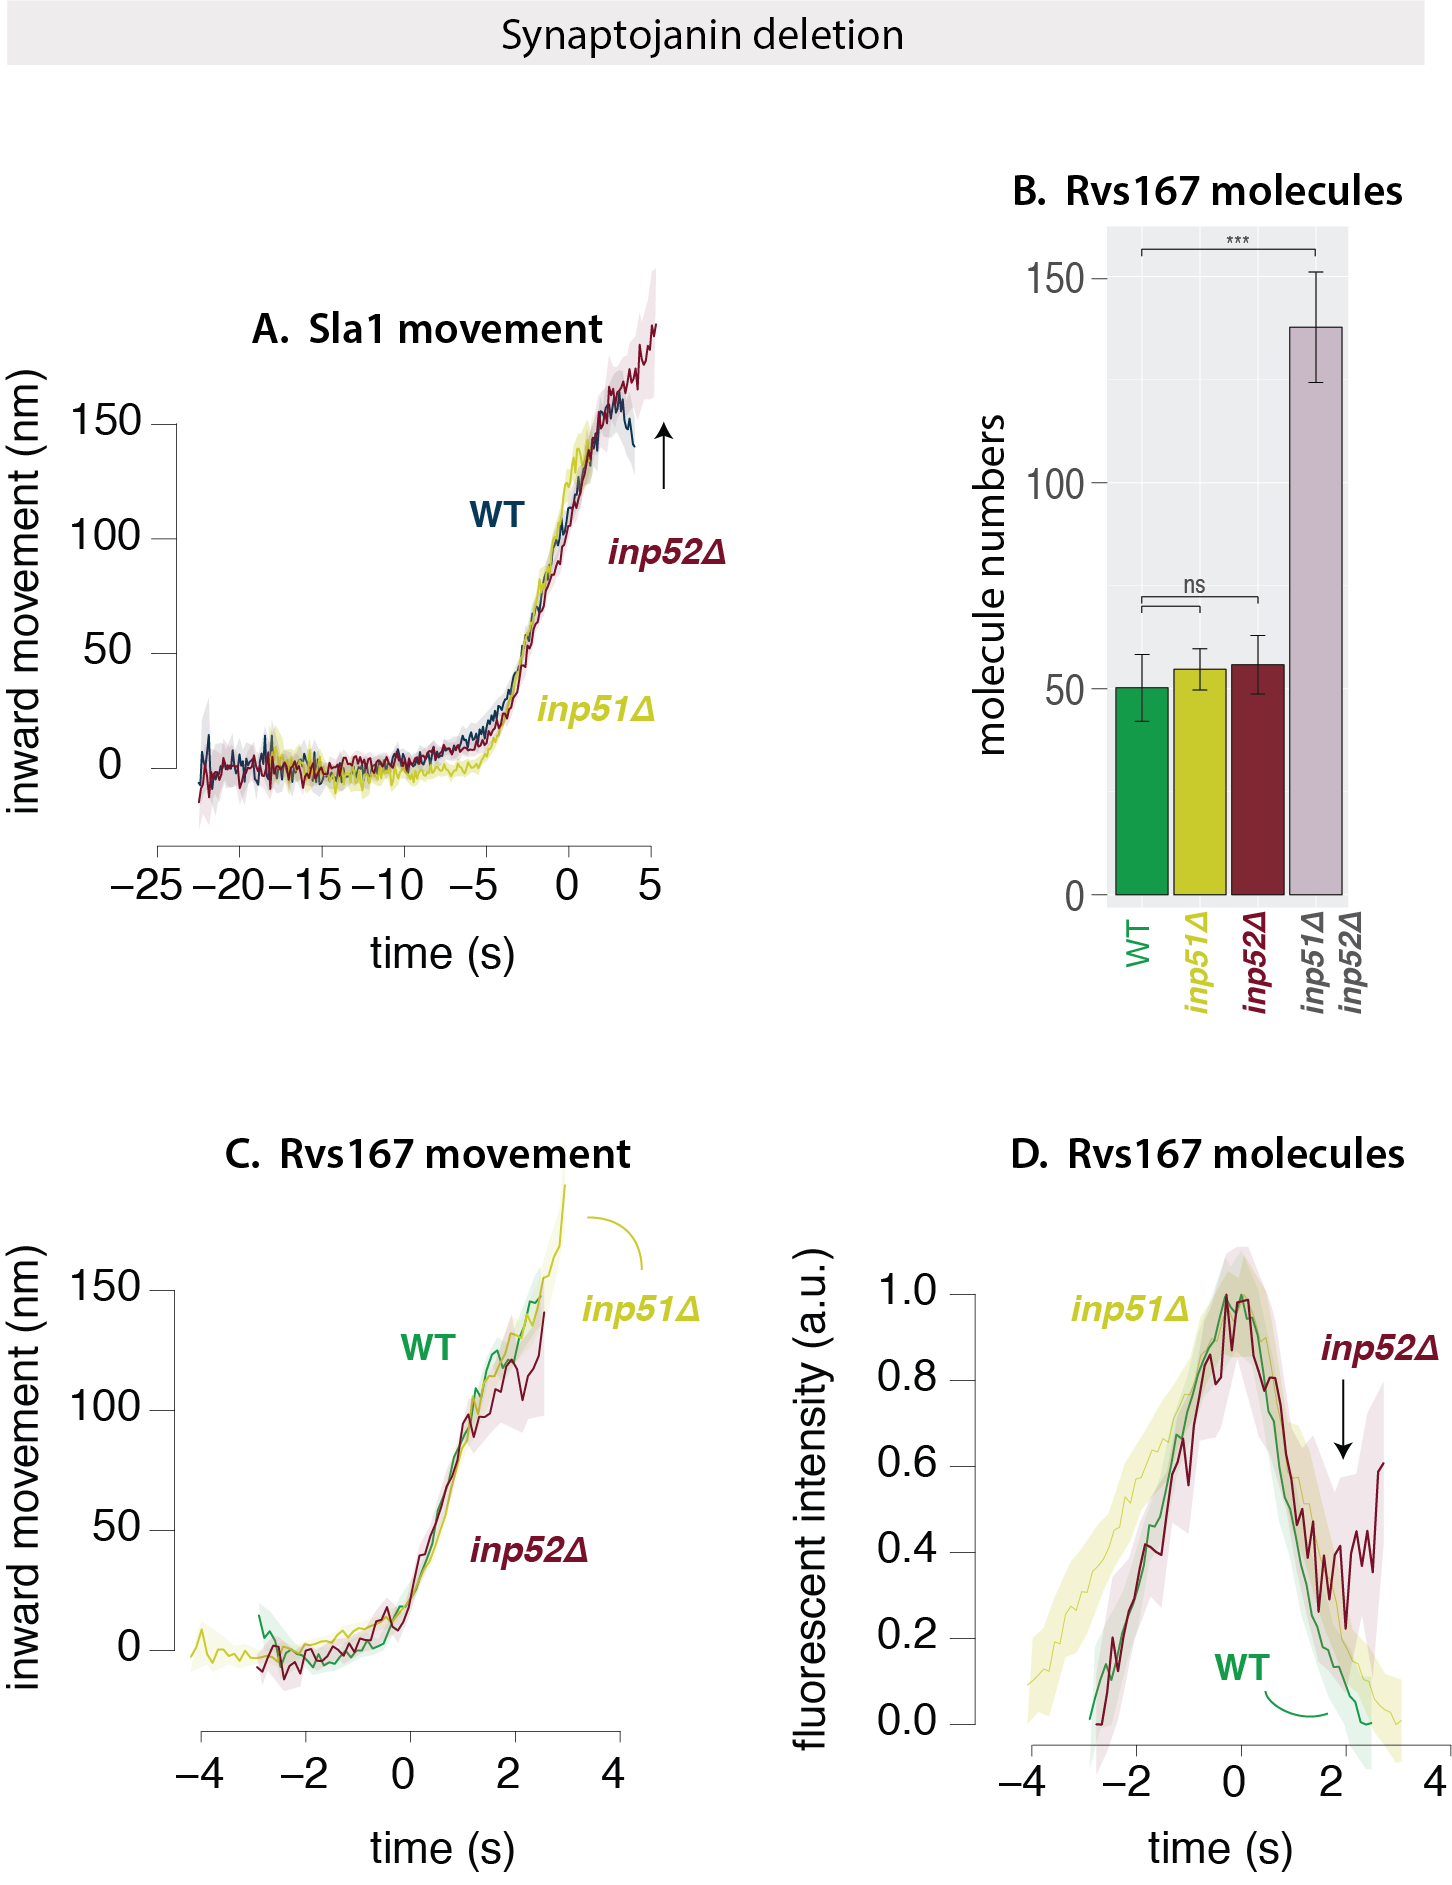
\includegraphics[width=17cm,height=17cm,keepaspectratio]{figures/results_final/inp_movement3}
		\caption{Sla1 and Rvs167 in Synaptojanin deletion \label{fig5}}
		\end{figure}		

	\vspace{5mm}
	I tested this model by investigating the effect of synaptojanin deletion on coat and scission proteins. First, of the three yeast Synaptojanins, only Inp52-GFP localizes to cortical patches. Dual-color imaging and time alignment with Abp1 as described in Picco et al., shows that Inp52 localizes to endocytic sites at the late stage of scission along with Rvs. The centroid of Inp52-GFP can be localized to the tip of the invaginated tube, consistent with the Liu theory of membrane scission: spatial and temporal localization is consistent with influence on scission. Inp51-GFP exhibits a diffuse cytoplasmic signal, while Inp53 localizes to patches within the cytoplasm, likely to the trans-golgi network, as has been noted in other work. 



	\vspace{5mm}
	Deletion of Inp52 does not affect the speed of membrane invagination, as reported by the movement of the Sla1 centroid. Sla1-GFP patches are assembled and disassembled, as are Rvs167-GFP patches. All Sla1-GFP patches in the movies analysed (n=13 cells) move inwards.  Dense clusters at bud neck are not considered. 72.9\% of Rvs167-GFP patches move inwards into the cytoplasm (n=4 cells, 37patches). Remaining patches are disassembled without apparent inward movement. Dense clusters at bud neck are not included in the statistics. Vesicle scission appears to occur similar to wild-type, since the Rvs167 centroid moves inwards to approximately the same distance into the cytoplasm, indicating that the base of the vesicles are likely at the same position as in wild-type. Both Sla1 and Rvs167 centroids however, persist post-scission (arrowheads in figure) instead of disassembling immediately like in the WT. Since majority of the patches move inwards, and the increase in the lifetime of Rvs is post-scission, I find that the data is consistent with a role for Inp52 in vesicle uncoating, rather than a primary role in membrane scission, with the aberrations in plasma membrane morphology consequent of failure to recycle components, rather than scission. 
	


	\vspace{5mm}
	Deletion of Inp51 does not affect Rvs167 or Sla1 centroid movement. All Sla1-GFP patches move inward (n=19 cells). 93\% of Rvs167-GFP patches move inward (n=3 cells, 44 patches), similar to WT. Assembly of Rvs167 in the Inp51del is slowed, the implication of this delay is not thus far clear. 


	
	\subsection{Does protein friction induce membrane scission? }
	
	Recent in-vitro experiments have proposed protein friction as a mechanism by which membrane scission could occur via BAR domain proteins in the absence of dynamin24. In this model, a BAR domain scaffold on a membrane tube forms a frictional barrier to lipid diffusion. Forces that pull on the membrane, such as those exerted by motor proteins like myosins or actin polymerization, increase the frictional force exerted by the scaffold on the underlying membrane tube, increasing membrane tension in the bare region of the tube caused by membrane thinning from the lack of lipid influx to this region. Eventually, membrane pores form in this portion of the tube, leading to breaking the tube, and formation of a vesicle. Such a friction-dependent membrane scission model would predict that if more BAR proteins are added to the membrane, frictional force would increase, and scission should occur faster, that is, at shorter invagination lengths than with fewer BAR proteins. Essentially, this model requires a friction-inducing BAR scaffold, and a force that pulls the membrane under it. In yeast CME, this combination is provided by the Rvs complex and polymerization of the actin network respectively. 
	

	\subparagraph{Membrane scission does not occur at shorter tube lengths when amount of Rvs is increased}
		\mbox{}\\
		
				\begin{figure}
			\centering
			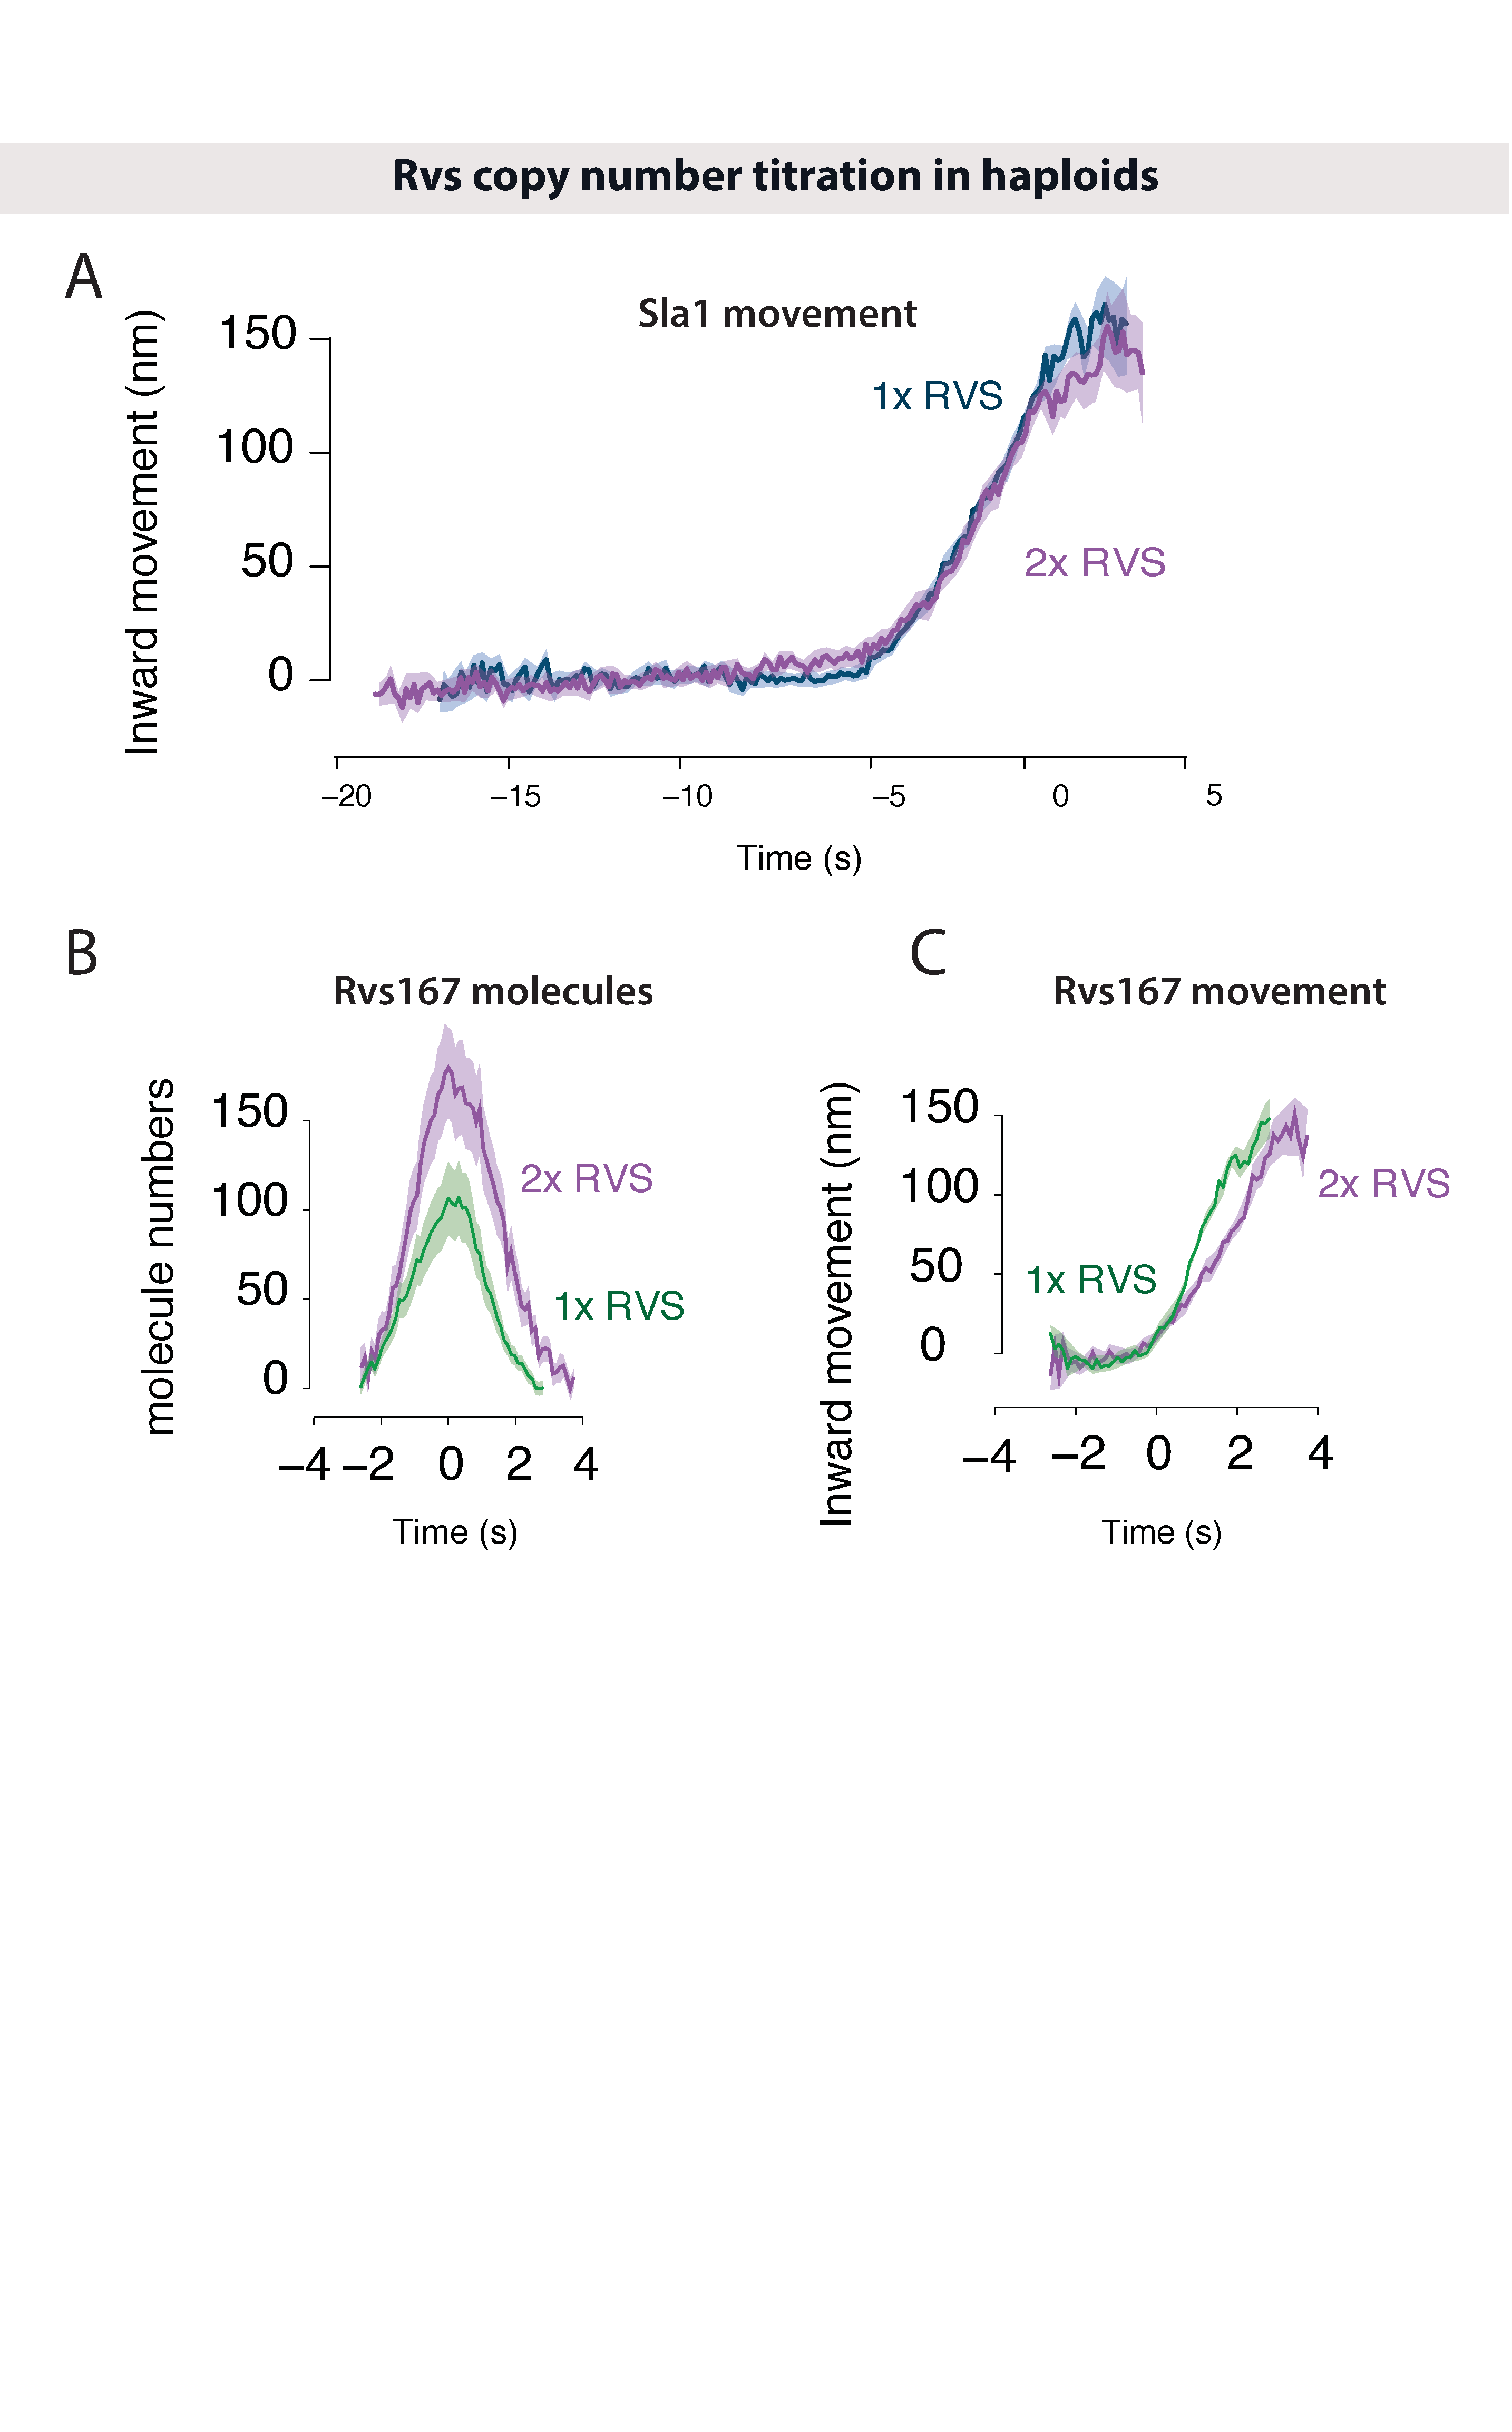
\includegraphics[width=15cm,height=15cm,keepaspectratio]{figures/results_final/rvs_haploid}
			\caption{Sla1 and Rvs167 in Synaptojanin deletion \label{fig5}}
		\end{figure}	
		

	To test whether protein friction could influence membrane scission in yeast, we duplicated the Rvs167 and Rvs161 genes as described in Huber et al.21. Gene duplication is performed in haploid cells to produce strains that have one (WT number) and two copies of both Rvs161 and Rvs167. These haploid strains are then crossed, so that diploid strains are generated that have 4x copies of the Rvs167 and Rvs161 genes, 2x copies each (WT number). Strains containing 1x copy of each Rvs is generated by crossing rvs167del strain with an rvs161del strain.
	


		\begin{figure}
	\centering
	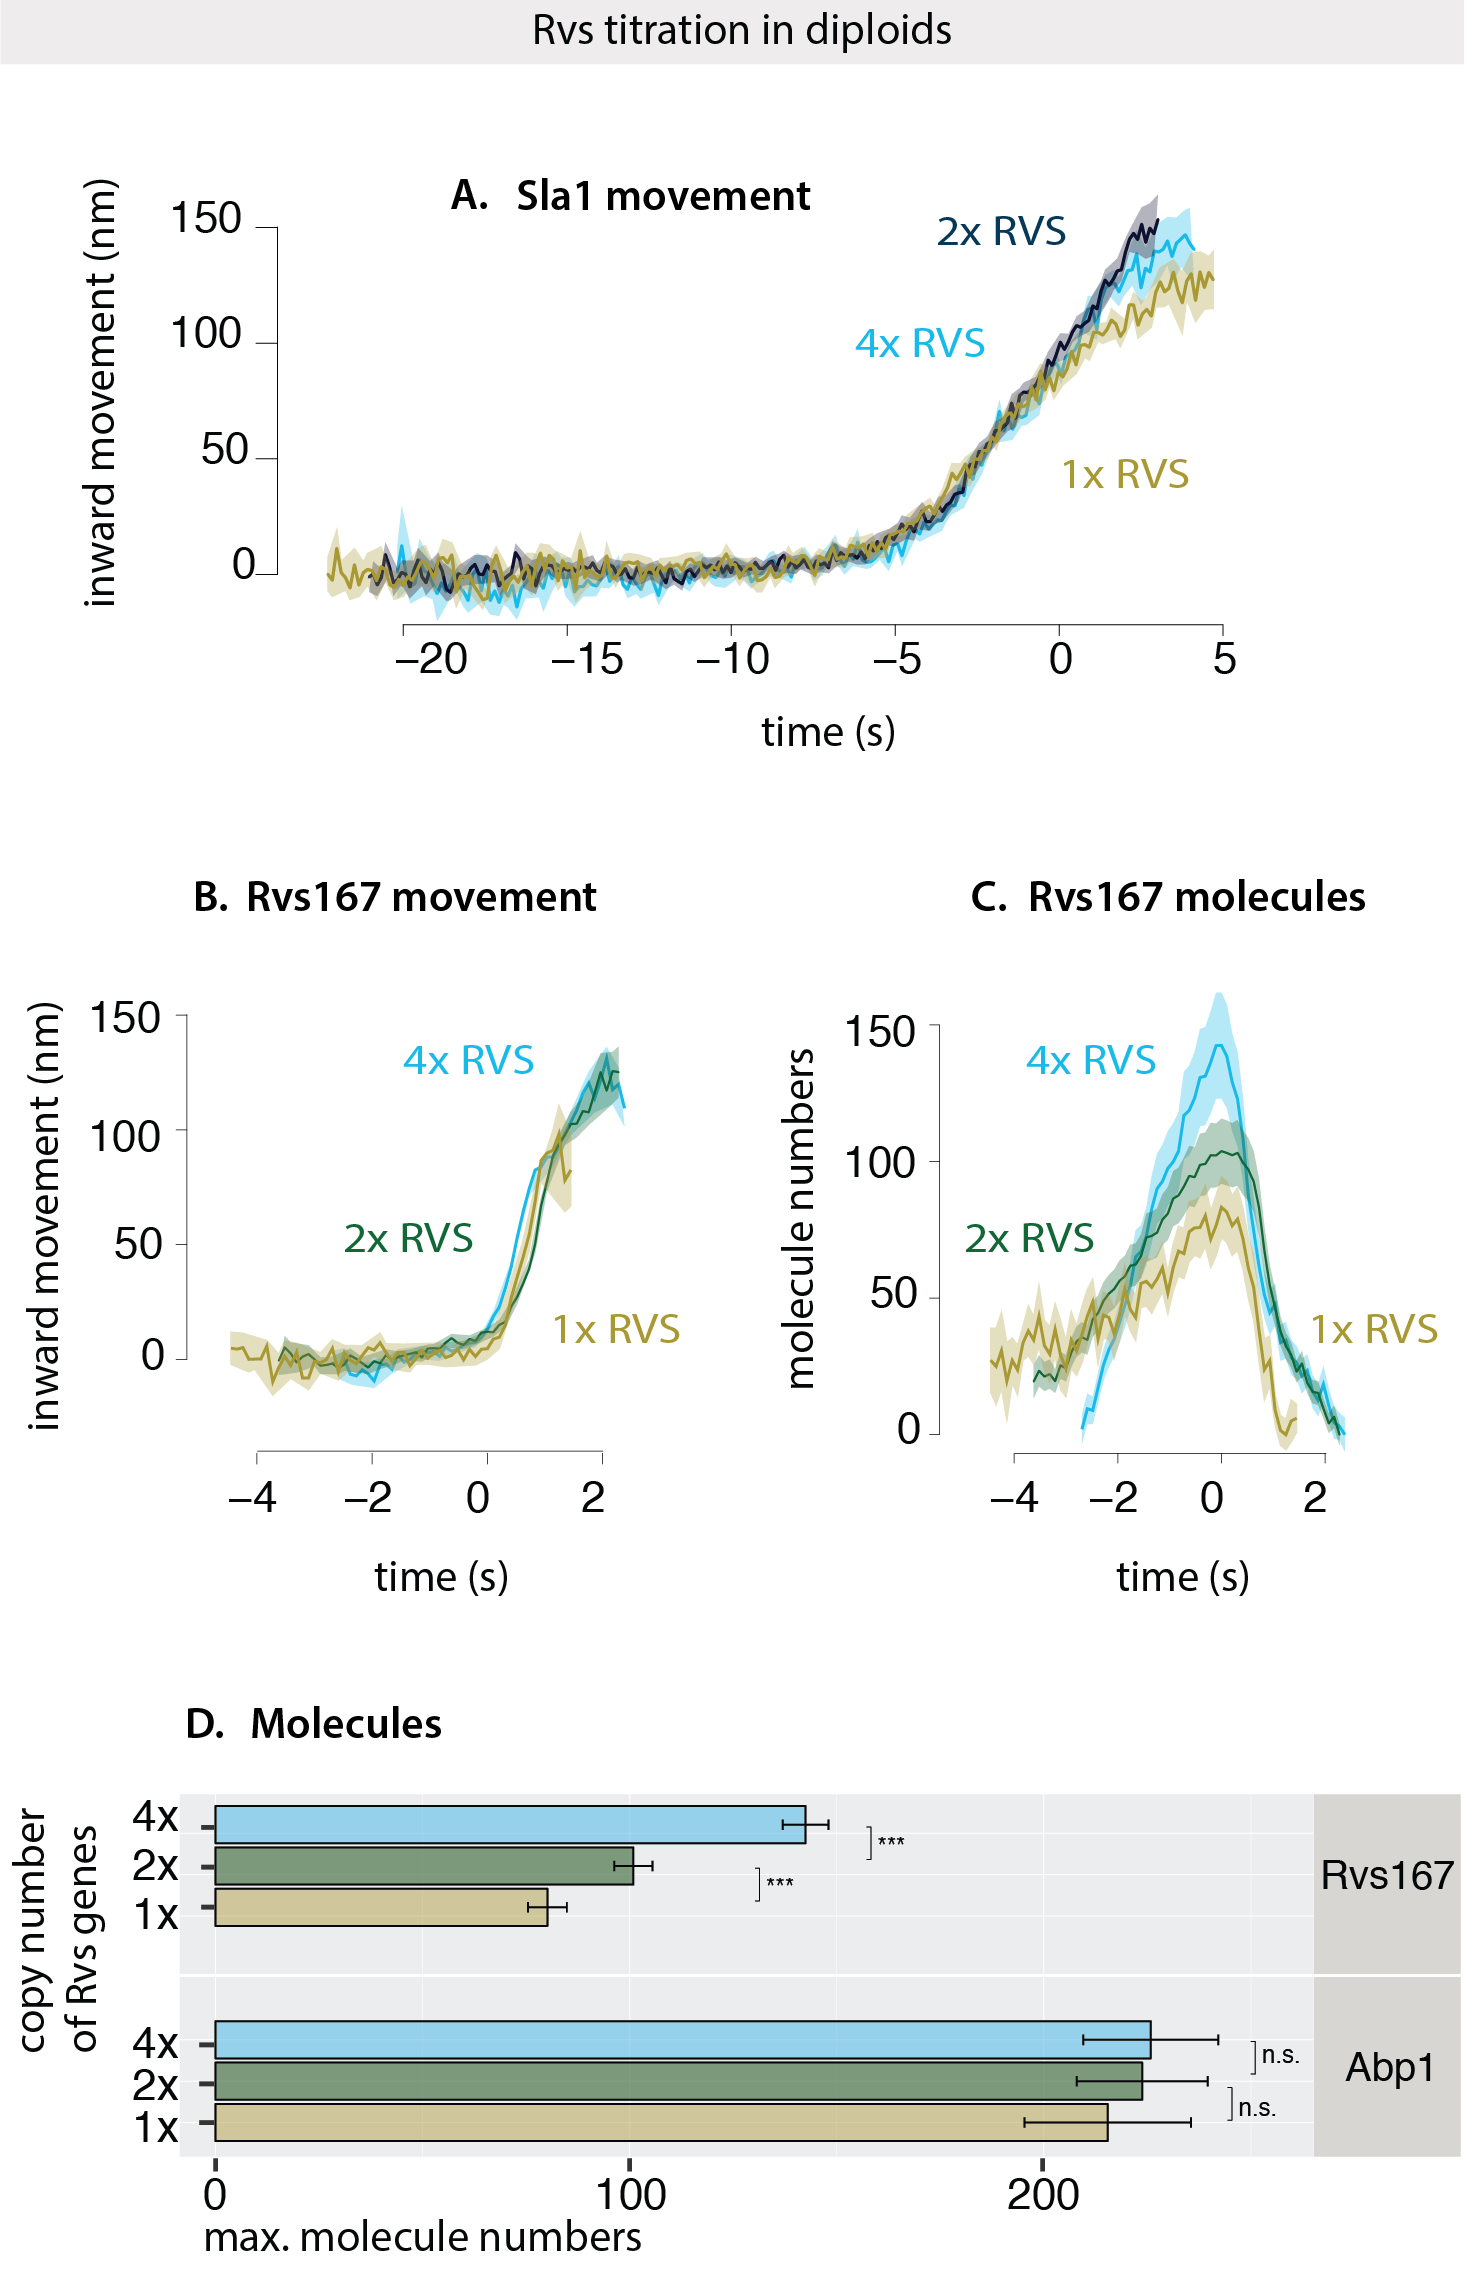
\includegraphics[width=21cm,height=21cm,keepaspectratio]{figures/results_final/protein_friction2}
	\caption{Sla1 and Rvs167 in Synaptojanin deletion \label{fig5}}
	\end{figure}

	\vspace{5mm}
	By quantifying the number of Rvs167 proteins as described in Picco et al., 12  first in the haploid strains, I found that in haploids, the average maximum number of Rvs molecules recruited to endocytic sites is 179.7328, SEM=10.1, compared to 113.505, SEM=5.2:  1.6x Rvs is recruited to endocytic sites in the duplicated strain compared to WT. The averaged trajectory of Sla1-GFP, however does not change between the 4x and 2x copies of Rvs: like in the WT, Sla1 moves in to 140nm. The dynamics of Rvs, however is chaged: In Fig.x , the centroid movement of both WT and 2x Rvs167-GFP (henceforth 2x Rvs) is aligned so that time=0 corresponds to the maxima of the fluorescent intensity, which corresponds to scission time. Molecule numbers of 2x Rvs increase at a faster rate than WT, and the disassembly is slowed by ~1 second. In the corresponding Rvs movement trace, instead of the sharp jump seen in WT, there is a delay in the movement into the cytoplasm.


	
	In diploid cells, recruitment of Rvs is similarly measured in the duplicated strain containing 4 copies of both RVS genes (4x Rvs), two copies strain (WT, 2x Rvs), and one copy of each (1x Rvs). Recruitment of Rvs is not directly proportionate to gene copy number: maximum number of Rvs recruited increases from 100.9, SEM=4.6 from in the 2x Rvs strain to 142.5, SEM=5.5 in the 4x strain. In the 1x Rvs strain, 80.2, SEM=4.7 molecules of Rvs are recruited before scission occurs. In order to determine whether this is a reflection on protein availability or if something else limits recruitment of Rvs, I quantified the cytoplasmic intensity of Rvs167-GFP in the respective strains by first producing z-stacks of time-lapse images of cells, and measuring the intensity within the cytoplasm (for details see METHODS). As can be seen in TABLE.X, the number of molecules recruited to endocytic sites scales with the amount of protein in the cytoplasm.  
	\vspace{5mm}
	
	Inward movement of the Rvs centroid is similar for the 4x, 2x and 1x Rvs: the jump inwards is about 80nm. In the 1x strain, however, the centroid disappears immediately after scission, suggesting that there is reduced Rvs at the base of the newly formed vesicle compared to the WT. Recruitment dynamics of all three are different: in the 4x Rvs strain, Rvs is recruited at a rate of 57 molecules/second, which is reduced to 27 molec/sec for the 2x and 19.07 molec/sec for the 1x strain. 

	\vspace{5mm}
	 Sla1 centroid movement, meanwhile is the same in 4x and 2x Rvs strains. In the 1x Rvs strain, Sla1 movement is slightly shifted, suggesting that vesicle scission occurs at invagination lengths about 10nm shorter than that as WT when fewer Rvs molecules are recruited, but increasing Rvs recruitment does not affect membrane progression. 


	
	\subsection{Scission timing is determined by actin forces, \\
		BAR domains prevent scission}
	
	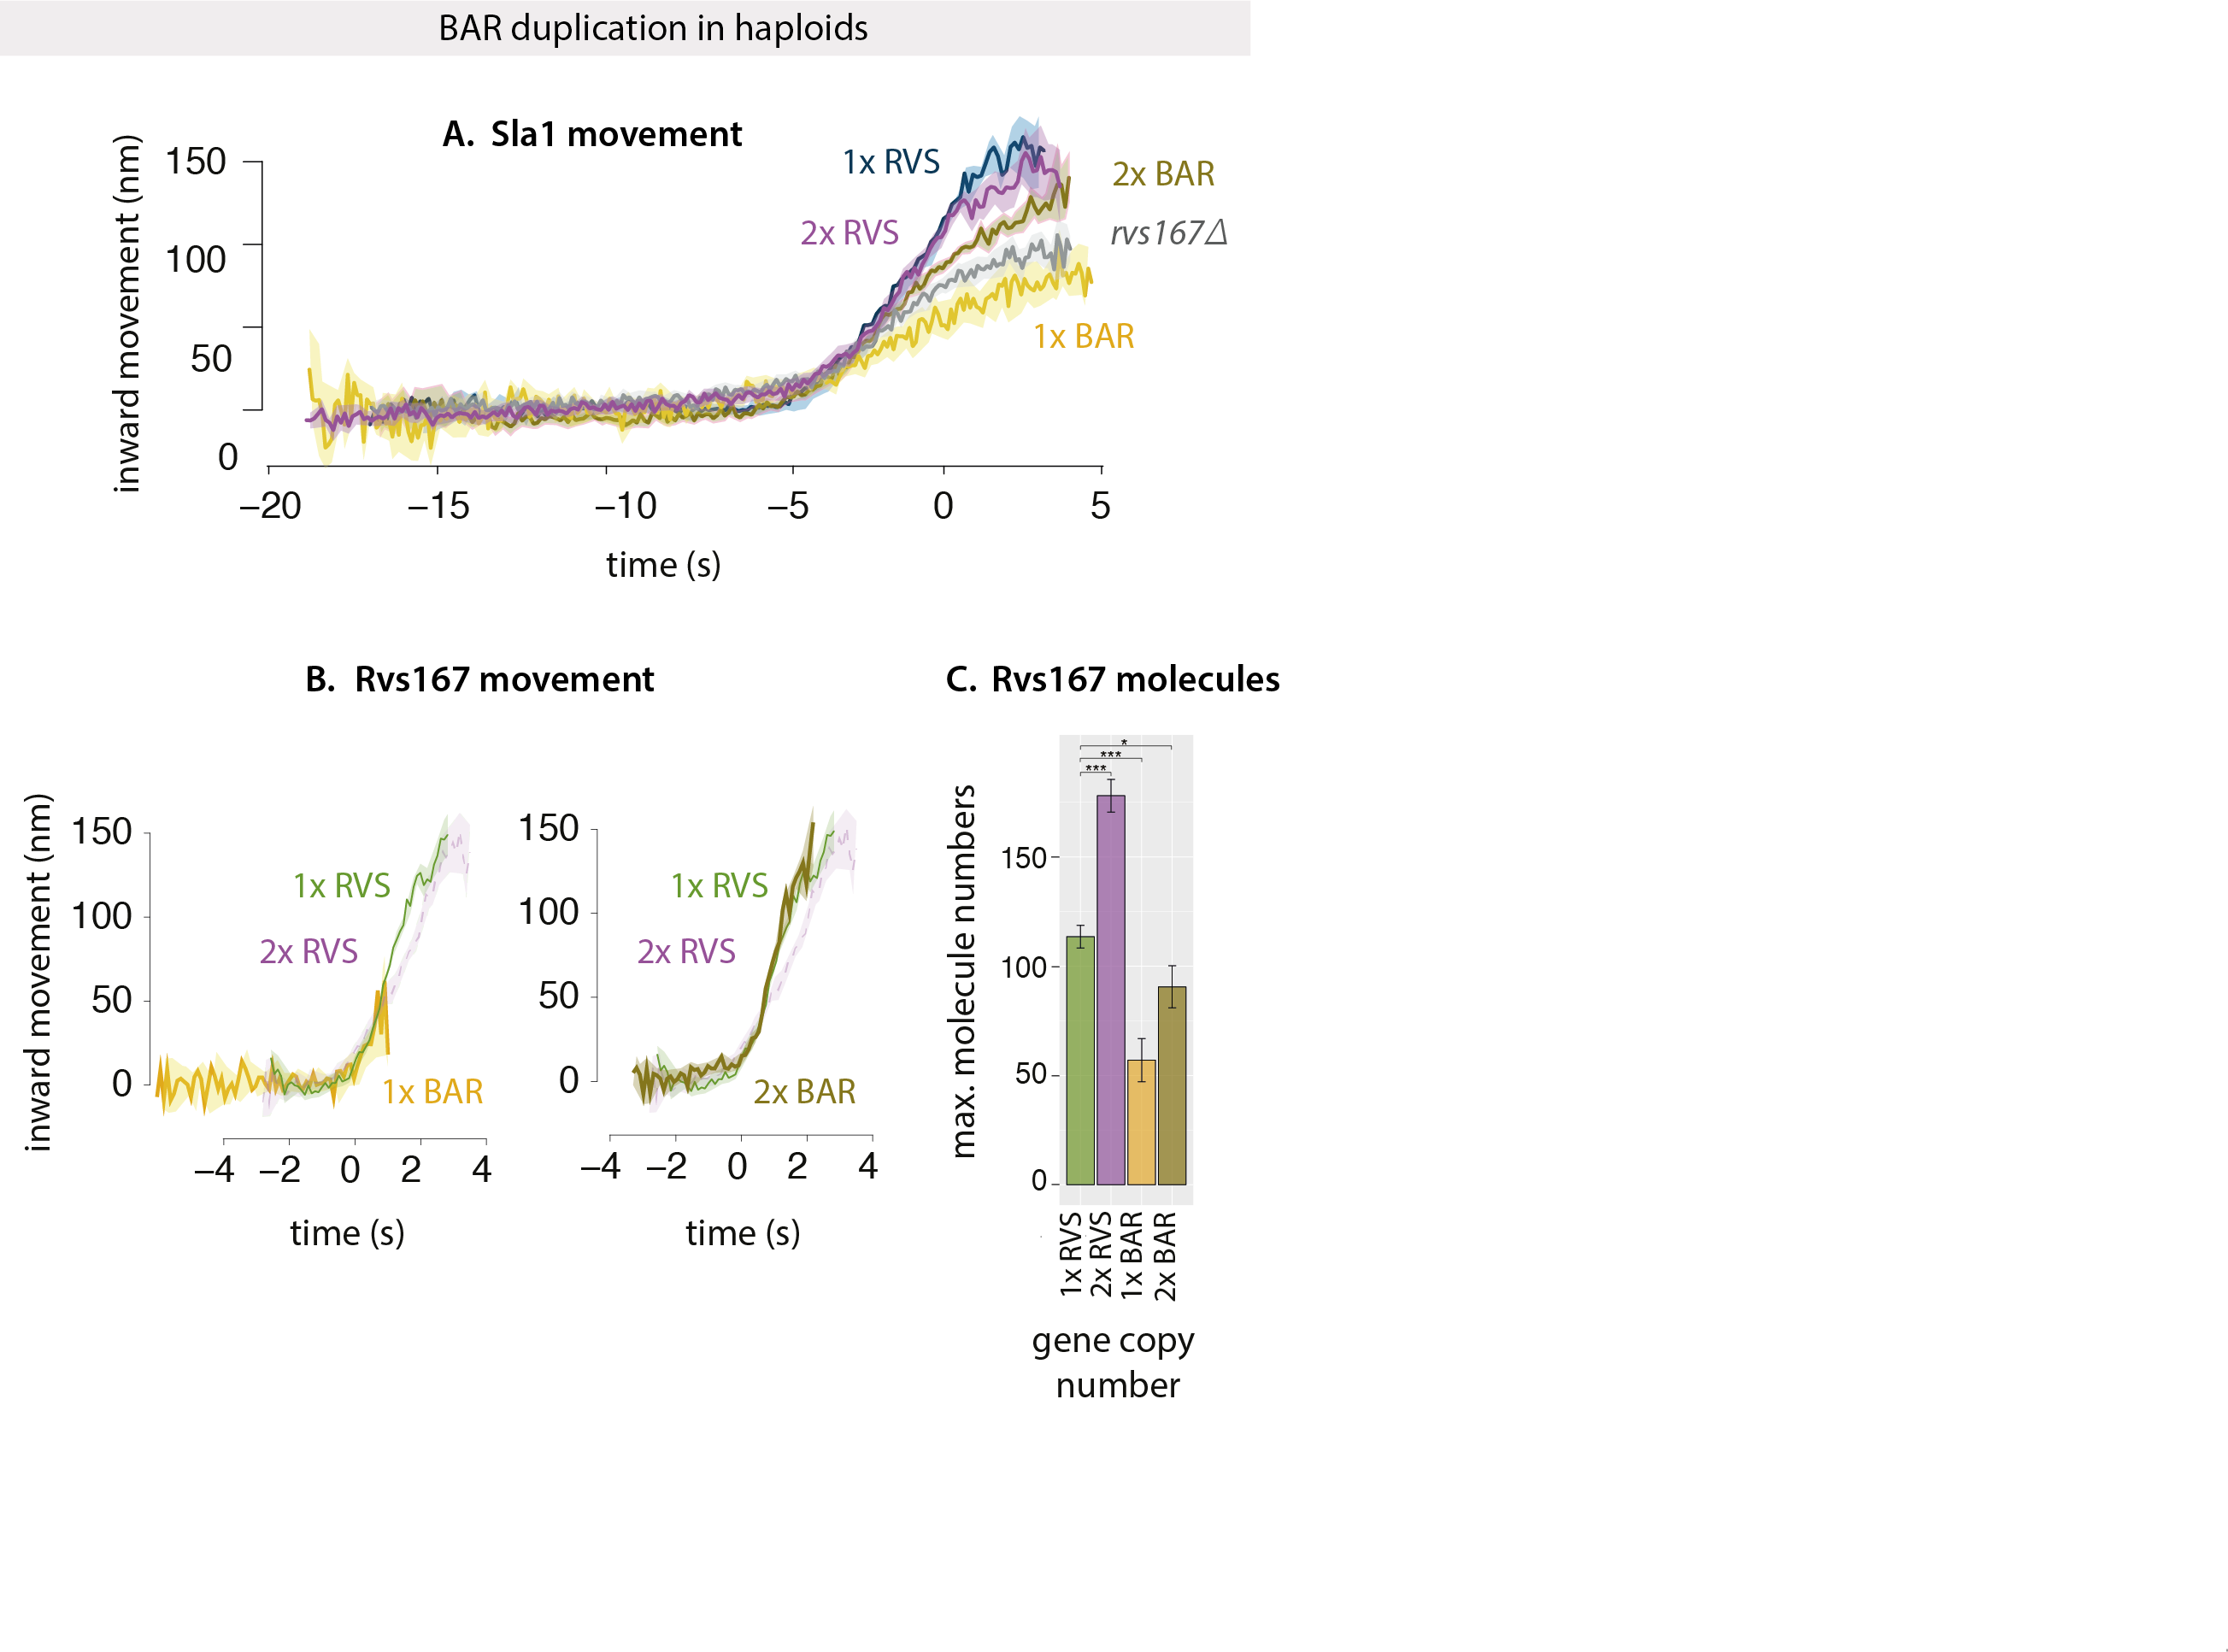
\includegraphics[width=23cm,height=23 cm,keepaspectratio]{figures/results_final/scaffolding_overlaid2}
	
	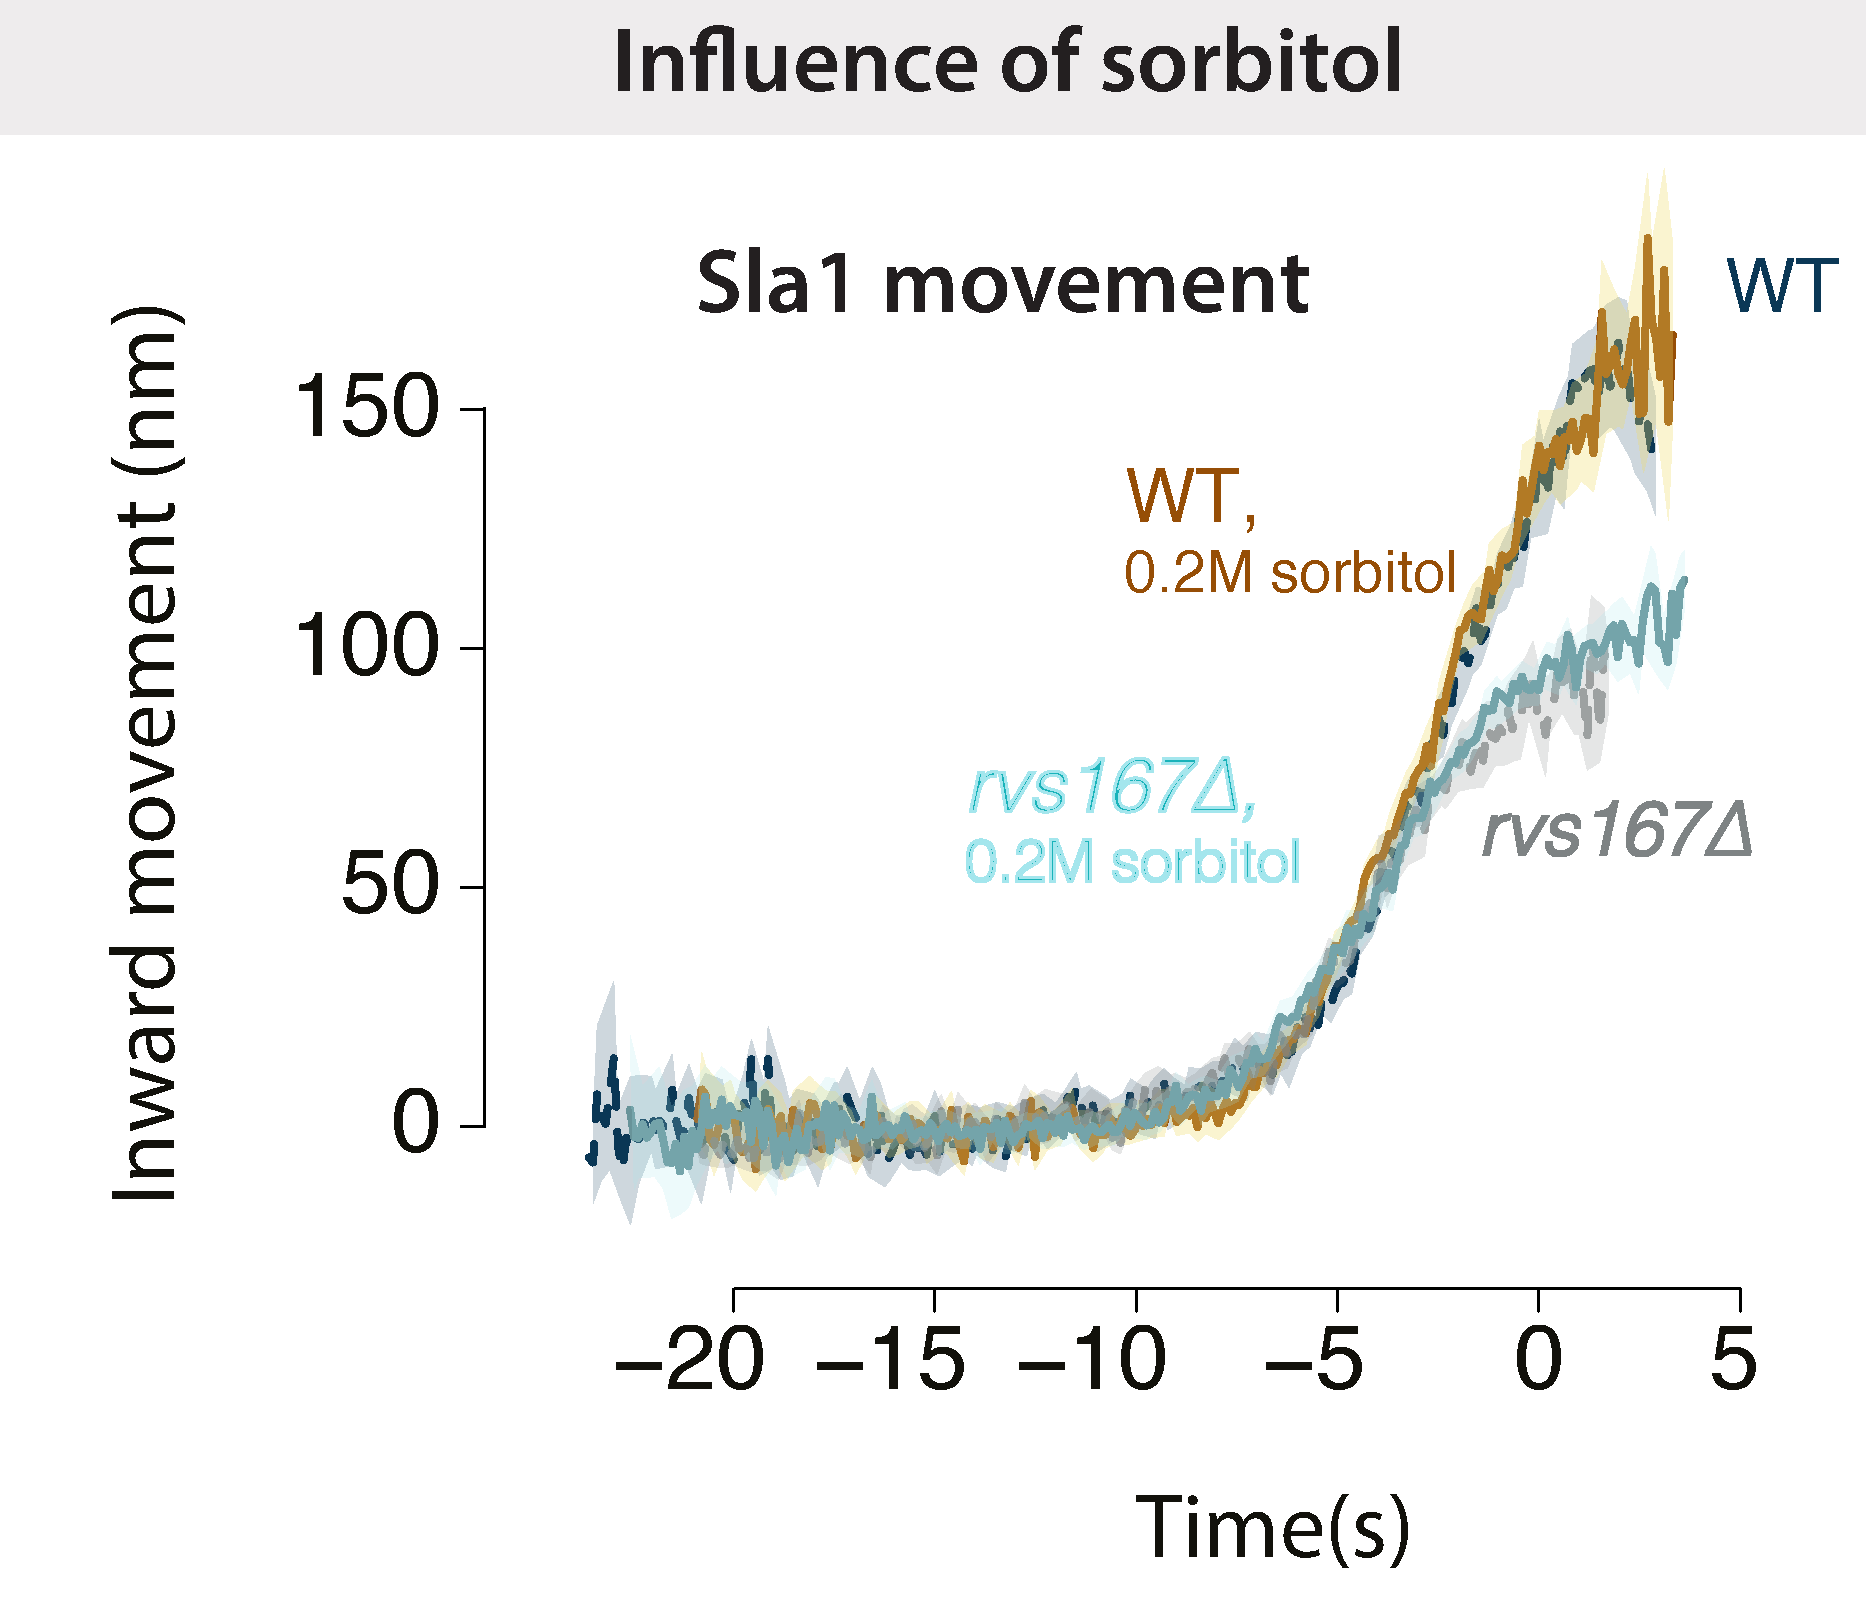
\includegraphics[width=14cm,height=14 cm,keepaspectratio]{figures/results_final/sorbitol}

\chapter{Discussion}    
\label{Ch:Discussion}

%\citep{Antonny2016}
Recruitment and function of the Rvs complex in has been explored in this work, as well as several models for how membrane scission could be effected in yeast endocytosis. 
I propose that Rvs localizes to endocytic sites by interactions of the BAR domains of the Rvs complex with invaginated membrane, and that the SH3 domain mediated protein-protein interactions are required for efficient recruitment of Rvs to sites. Arrival of Rvs on membrane tube scaffolds the membrane and prevents premature membrane scission,till actin forces rupture the membrane, causing vesicle scission. Effective scaffolding depends on recruitment of a critical number of Rvs molecules. Here I discuss the main findings of this thesis in support of these propositions.



\section{Recruitment of Rvs to endocytic sites}
Rvs is relatively short-lived protein at endocytic sites. It is recruited only once membrane tube is formed (Kaksonen, Toret and Drubin, 2005; Kukulski et al., 2012; Picco et al., 2015). Fluorescence correlation spectroscopy (FCS) measurements have shown that the cytosolic concentration of Rvs167 and Rvs161 is quite high compared to other endocytic proteins (Boeke et al., 2014). Many endocytic proteins like Las17, Vrp1, type1 myosins, are measured at 80-240nM, while cytosolic concentration of Rvs161 and 167 is 721nM and 354nM respectively. In spite of this, relatively few numbers of Rvs are recruited to endocytic sites, suggesting that cytosolic concentration does not determine recruitment. Comparison between FCS measurements of cytoplasmic concentration for different endocytic proteins, and their recruitment to the endocytic sites indicates low correlation between the two, perhaps unsurprisingly, requiring that other directed mechanisms recruit proteins in a timed and efficient manner. In the case of Rvs, both timing and efficiency appear crucial to its function, the question is what confers both. 



%\subsection{Timing of localization and efficiency of recruitment}

\subsection{The BAR domain senses membrane curvature}
The curved structure of BAR dimers (Peter et al., 2004; Mim et al., 2012) has suggested that Rvs is recruited by its preference for some membrane shapes over others, supported by its arrival at curved membrane tubes. In the absence of membrane curvature, in \textit{sla2$\Delta$} cells, the BAR domain alone does not localize to cortical patches (Fig.\ref{fig2_sla2del}D-F). This demonstrates for the first time that the BAR domain does indeed sense and requires membrane curvature to localize to cortical patches. Work on BAR domains have proposed that electrostatic interactions at the concave surface and tips of the BAR domain structure  mediate membrane binding (Qualmann, Koch and Kessels, 2011). Mutations in these lipid-binding surfaces would clarify the interaction with underlying lipids, and test if Rvs relies on similar interactions.



\subsection{BAR domain times recruitment of Rvs} 

BAR is able to localize to endocytic sites, and has a similar lifetime in WT cells (Fig.\ref{fig2_sla2del}, Fig.\ref{delsh3_movement}). In Fig.\ref{delsh3_movement}B we see that while the full-length Rvs167 arrives about 4 seconds after the arrival of Abp1, BAR arrives only 6 seconds after Abp1 arrives. There is a time delay between Abp1 recruitment and BAR arrival, compared to the arrival of full-length Rvs167, confirmed by the TIRF measurement in \ref{delsh3_movement}D. 

	\vspace{5mm}
The delay in recruitment could occur because the membrane has not acquired the required invagination length or because the loss of the SH3 domain causes delayed recruitment. That the delayed recruitment occurs because the invagination takes longer to reach a particular length is supported by the fact that Sla1 moves inwards at a slower rate in BAR cells. It takes longer for the membrane in BAR cells to reach the same length as WT. Rvs167 arrives in BAR cells when Sla1 has moved inwards 25-30nm (dashed red lines in Fig.\ref{delsh3_movement}A), which is also the distance Sla1 has moved when Rvs167 arrives in WT. By the time Sla1 has moved this distance, the membrane is already tubular (Kukulski et al., 2012; Picco et al., 2015), consistent with Rvs arrival at invaginated tubes. This suggests Rvs recruitment is timed to specific membrane invagination length- therefore to a specific membrane curvature- and that this timing is provided by the BAR domain. 



\subsection{The SH3 domain makes Rvs recruitment efficient} 
As seen in Fig.\ref{delsh3_movement}C, Rvs167 in BAR cells accumulates to about half the WT number, even though the same cytoplasmic concentration is measured. This indicates that the SH3 domain increases the efficiency of recruitment of Rvs. Either SH3 domain helps recruitment to endocytic sites, or it stabilizes interaction with sites. In \textit{sla2$\Delta$}  cells, full-length Rvs can assemble on the membrane (Fig.\ref{fig2_sla2del}D-F). Since BAR domains alone do not localize to patches in \textit{sla2$\Delta$}  cells, full-length localization must be mediated by the SH3 domain, supporting a role for the SH3 domain in increasing recruitment of Rvs by clustering protein molecules. 


\subsection{The SH3 domain can assemble and disassemble Rvs molecules independent of the BAR domain and actin interactions} 
As mentioned above, in \textit{sla2$\Delta$}  cells, full-length Rvs167 is able to assemble and disassemble at cortical patches without the curvature-dependent interaction of the BAR domain (Fig.\ref{fig2_sla2del}D-F). This unexpected finding indicates that the SH3 domain is able to mediate both the recruitment and the disassembly of Rvs at the endocytic site. 


	\vspace{5mm}
In \textit{sla2$\Delta$}  cells treated with LatA (Fig.\ref{fig2_sla2del}G-H), actin-based membrane curvature is inhibited, and the actin patch proteins are removed from the plasma membrane. Full-length Rvs167 in these cells still shows transient localizations at the plasma membrane (Fig.\ref{fig2_sla2del}A). In \textit{sla2$\Delta$} cells treated with LatA, the localization of BAR is lost. This suggests that localization of the full-length Rvs167 in LatA treated cells is dependent on an SH3 domain interaction, and that this is independent of both actin and membrane curvature. 


\subsection{SH3 domain affects actin dynamics}
In WT cells, the Abp1 and Rvs167 fluorescent intensities reach maxima concomitantly, and the consequent decay of both also coincide. That this occurs at the same time indicates that upon vesicle scission, the actin network is immediately disassembled. Membrane scission essentially occurs around the intensity peak of the two proteins. This coincident peak is lost in BAR cells. Rvs in these cells peaks several seconds after Abp1 intensity starts to drop, and the decay of Abp1 is prolonged, taking nearly double the time as in WT. As we see in Fig.\ref{delsh3_movement}C, the number of Abp1 molecules recruited is decreased to about two thirds the WT number. Although it is not clear what the decoupling of Abp1 and Rvs peaks means, the changes in Abp1 dynamics suggests a strong disruption of the actin network. SH3 domains are known to interact with components of the actin network like Abp1 and Las17 (Lila and Drubin, 1997, Madania et al., 1999), but study of other components of the actin machinery will be required to understand how exactly loss of the SH3 has changed the progression of endocytosis.  


\subsection{What does the SH3 domain interact with?}
SH3 interaction with an endocytic binding partner could help recruit Rvs to endocytic sites. Many such interaction partners have been proposed. Abp1 interaction with the Rvs167 SH3 domain has been shown (Lila and Drubin, 1997; Colwill et al., 1999), as has one with WASP protein Las17 (Madania et al., 1999; Liu et al., 2009), yeast Calmodulin Cmd1 (Myers et al., 2016), type I myosins (Geli et al., 2000), and Vrp1 (Lila and Drubin, 1997). These proteins are currently being studied as potential targets of the Rvs167 SH3 domain. All of these suggested binding partners localize to the base of the invagination (Yidi Sun, 2006; Picco et al., 2015), and do not follow the invaginating membrane into the cytoplasm. If one of these is the SH3 interaction partner, SH3 domains interact with the endocytic network at the base of the invagination. Centroid tracking however, suggests that Rvs is accumulated all over the membrane tube without bias towards the base of the invagination. If Rvs was recruited to the base and pulled up as the invagination grows, the centroid would move continuously upwards rather than remain relatively non-motile before the jump at scission time. It is possible that the SH3 initially helps cluster near the base, and as the membrane invaginations grow longer, BAR-membrane interactions dominate. 





\subsection{Total number of Rvs recruited is independent of ploidy}
When ploidy is doubled from haploids to diploids, we could expect that double the protein amount is expressed and recruited, but it does not appear so. The amount of Rvs recruited in WT haploid (1xh) and diploids (2xd) remains about the same, and cytoplasmic signal is similar (Fig.\ref{disc_conc}). This invariance between accumulated protein in haploids and diploids shows that Rvs recruitment is not determined by the number of alleles of Rvs. Haploid and diploid cells appear to tune the amount of Rvs recruitment to get a specific amount to endocytic sites.

	\begin{figure}[H]
	\centering
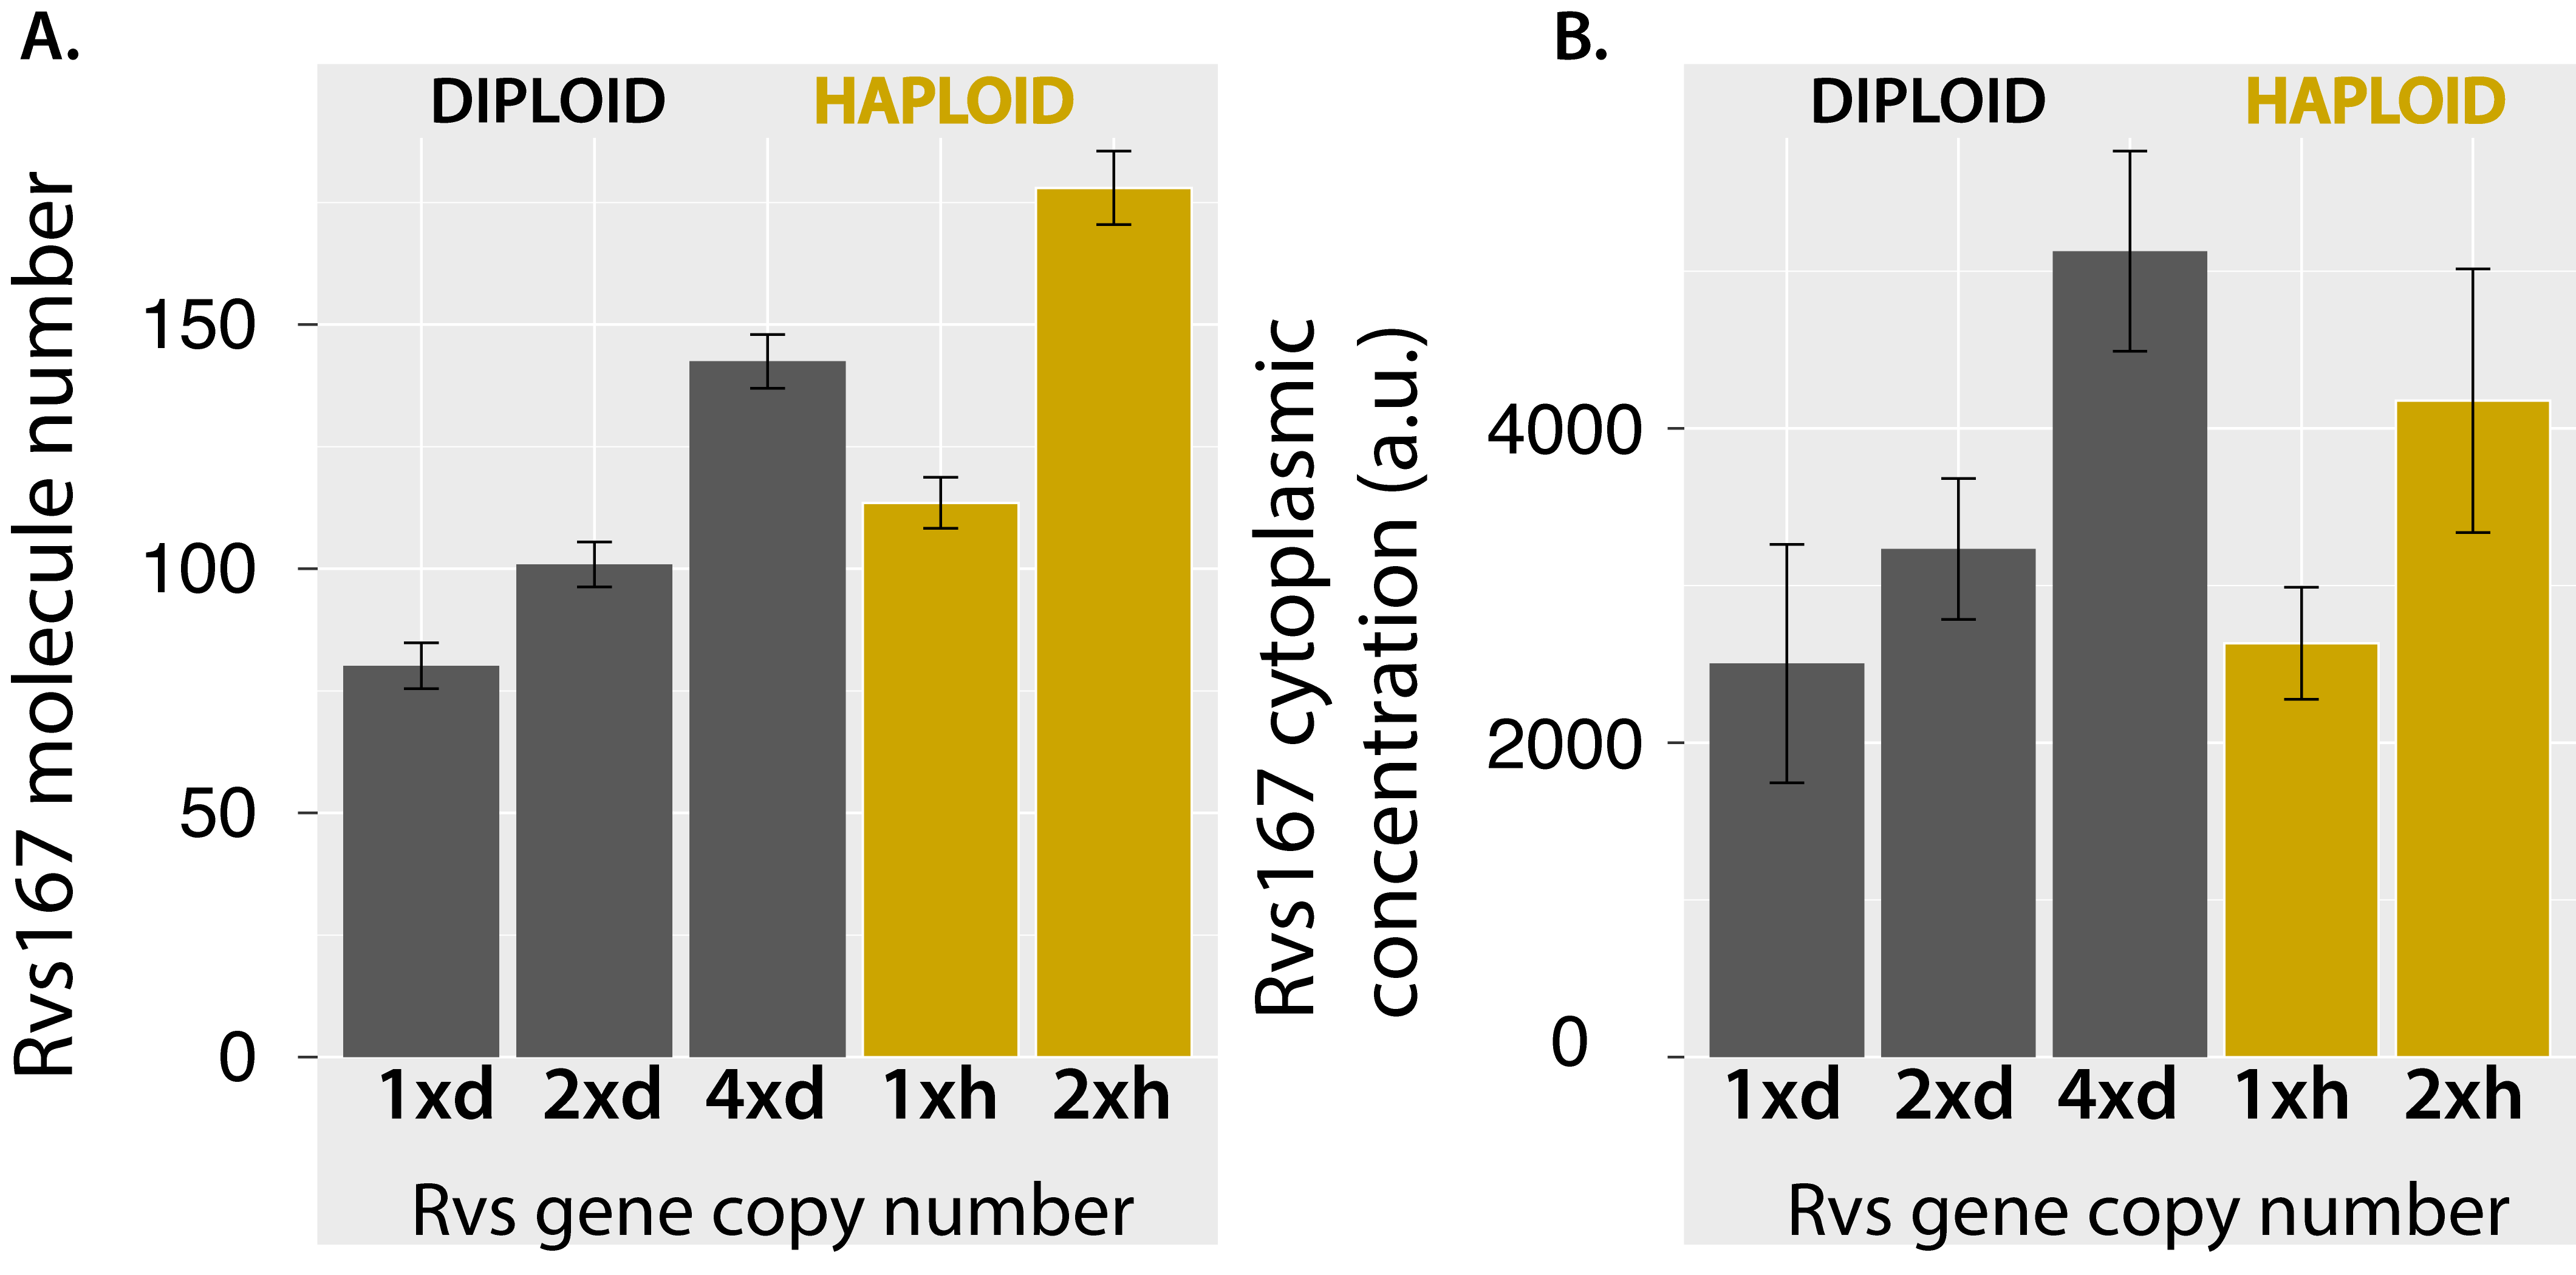
\includegraphics[width=12.5cm,height=12.5cm,keepaspectratio]{figures/discussion/number_comp}
	\caption[Recruitment of Rvs]
	{A. Maximum molecule number of Rvs167-GFP recruited with S.E.M in haploid and diploid cells with different gene copies of Rvs. 
	B. Cytoplasmic signal of Rvs167-GFP with standard deviation in haploid and diploid cells with different gene copies of Rvs. 
\label{disc_conc}}
	\end{figure}
%	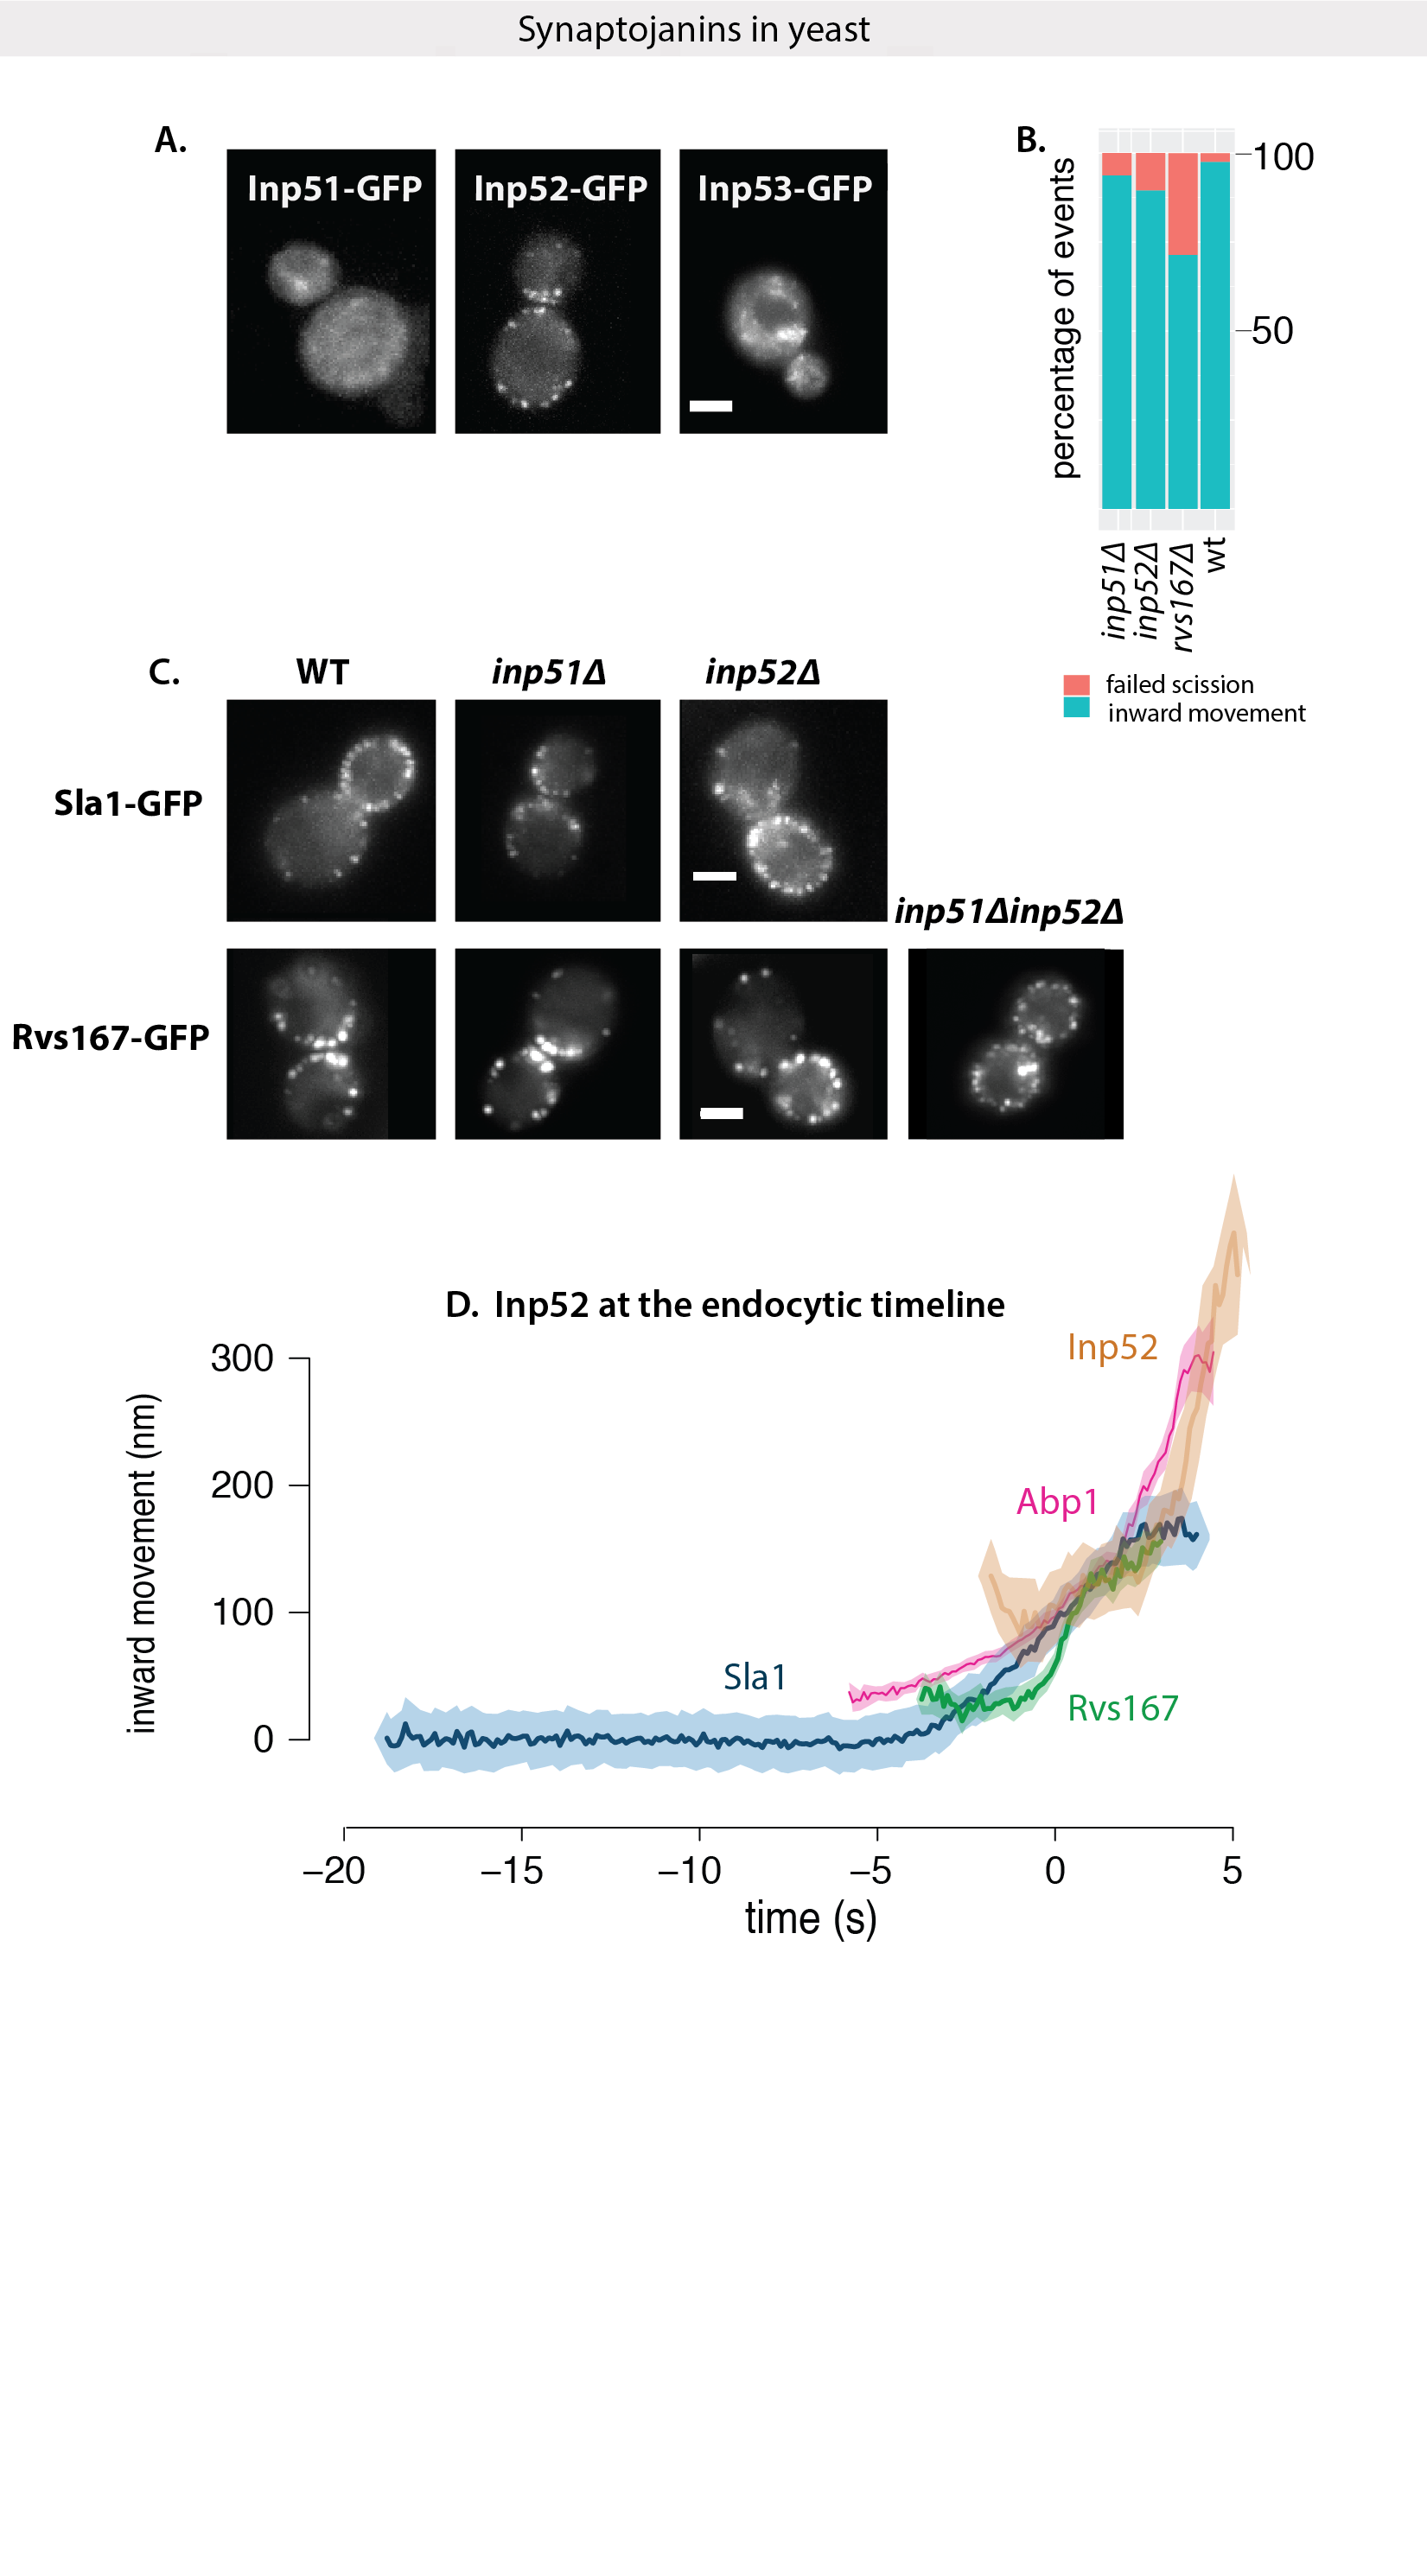
\includegraphics[width=19cm,height=19cm,keepaspectratio]{figures/results_final/inp}

\subsection{Rvs recruitment rate increases with increasing gene copy number}
 WT diploids (2xd) contain two copies each of RVS161 and RVS167 genes. Rvs duplicated diploids, which contain four copies each of RVS167 and RVS161 (4xd) could be expected to express and recruit to sites twice the amount of Rvs as 2xd. However, compared to 2xd, cytoplasmic signal in 4xd increases by 1.6x and recruitment of Rvs167 to endocytic sites increases only by 1.4x. Doubling the gene copy number increases, but does not double protein expression or recruitment in the case of Rvs. Similarly, duplicating Rvs genes in haploid cells results in an increase in number of molecules recruited, but not in doubling (1xh, 2xh). Although the rate of adding Rvs is different in haploids and diploids, in both cases, it increases by gene copy number (yellow line in Fig.\ref{disc_recruit_rate}). 

	\begin{figure}[H]
	\centering
	\hspace{-1cm}
	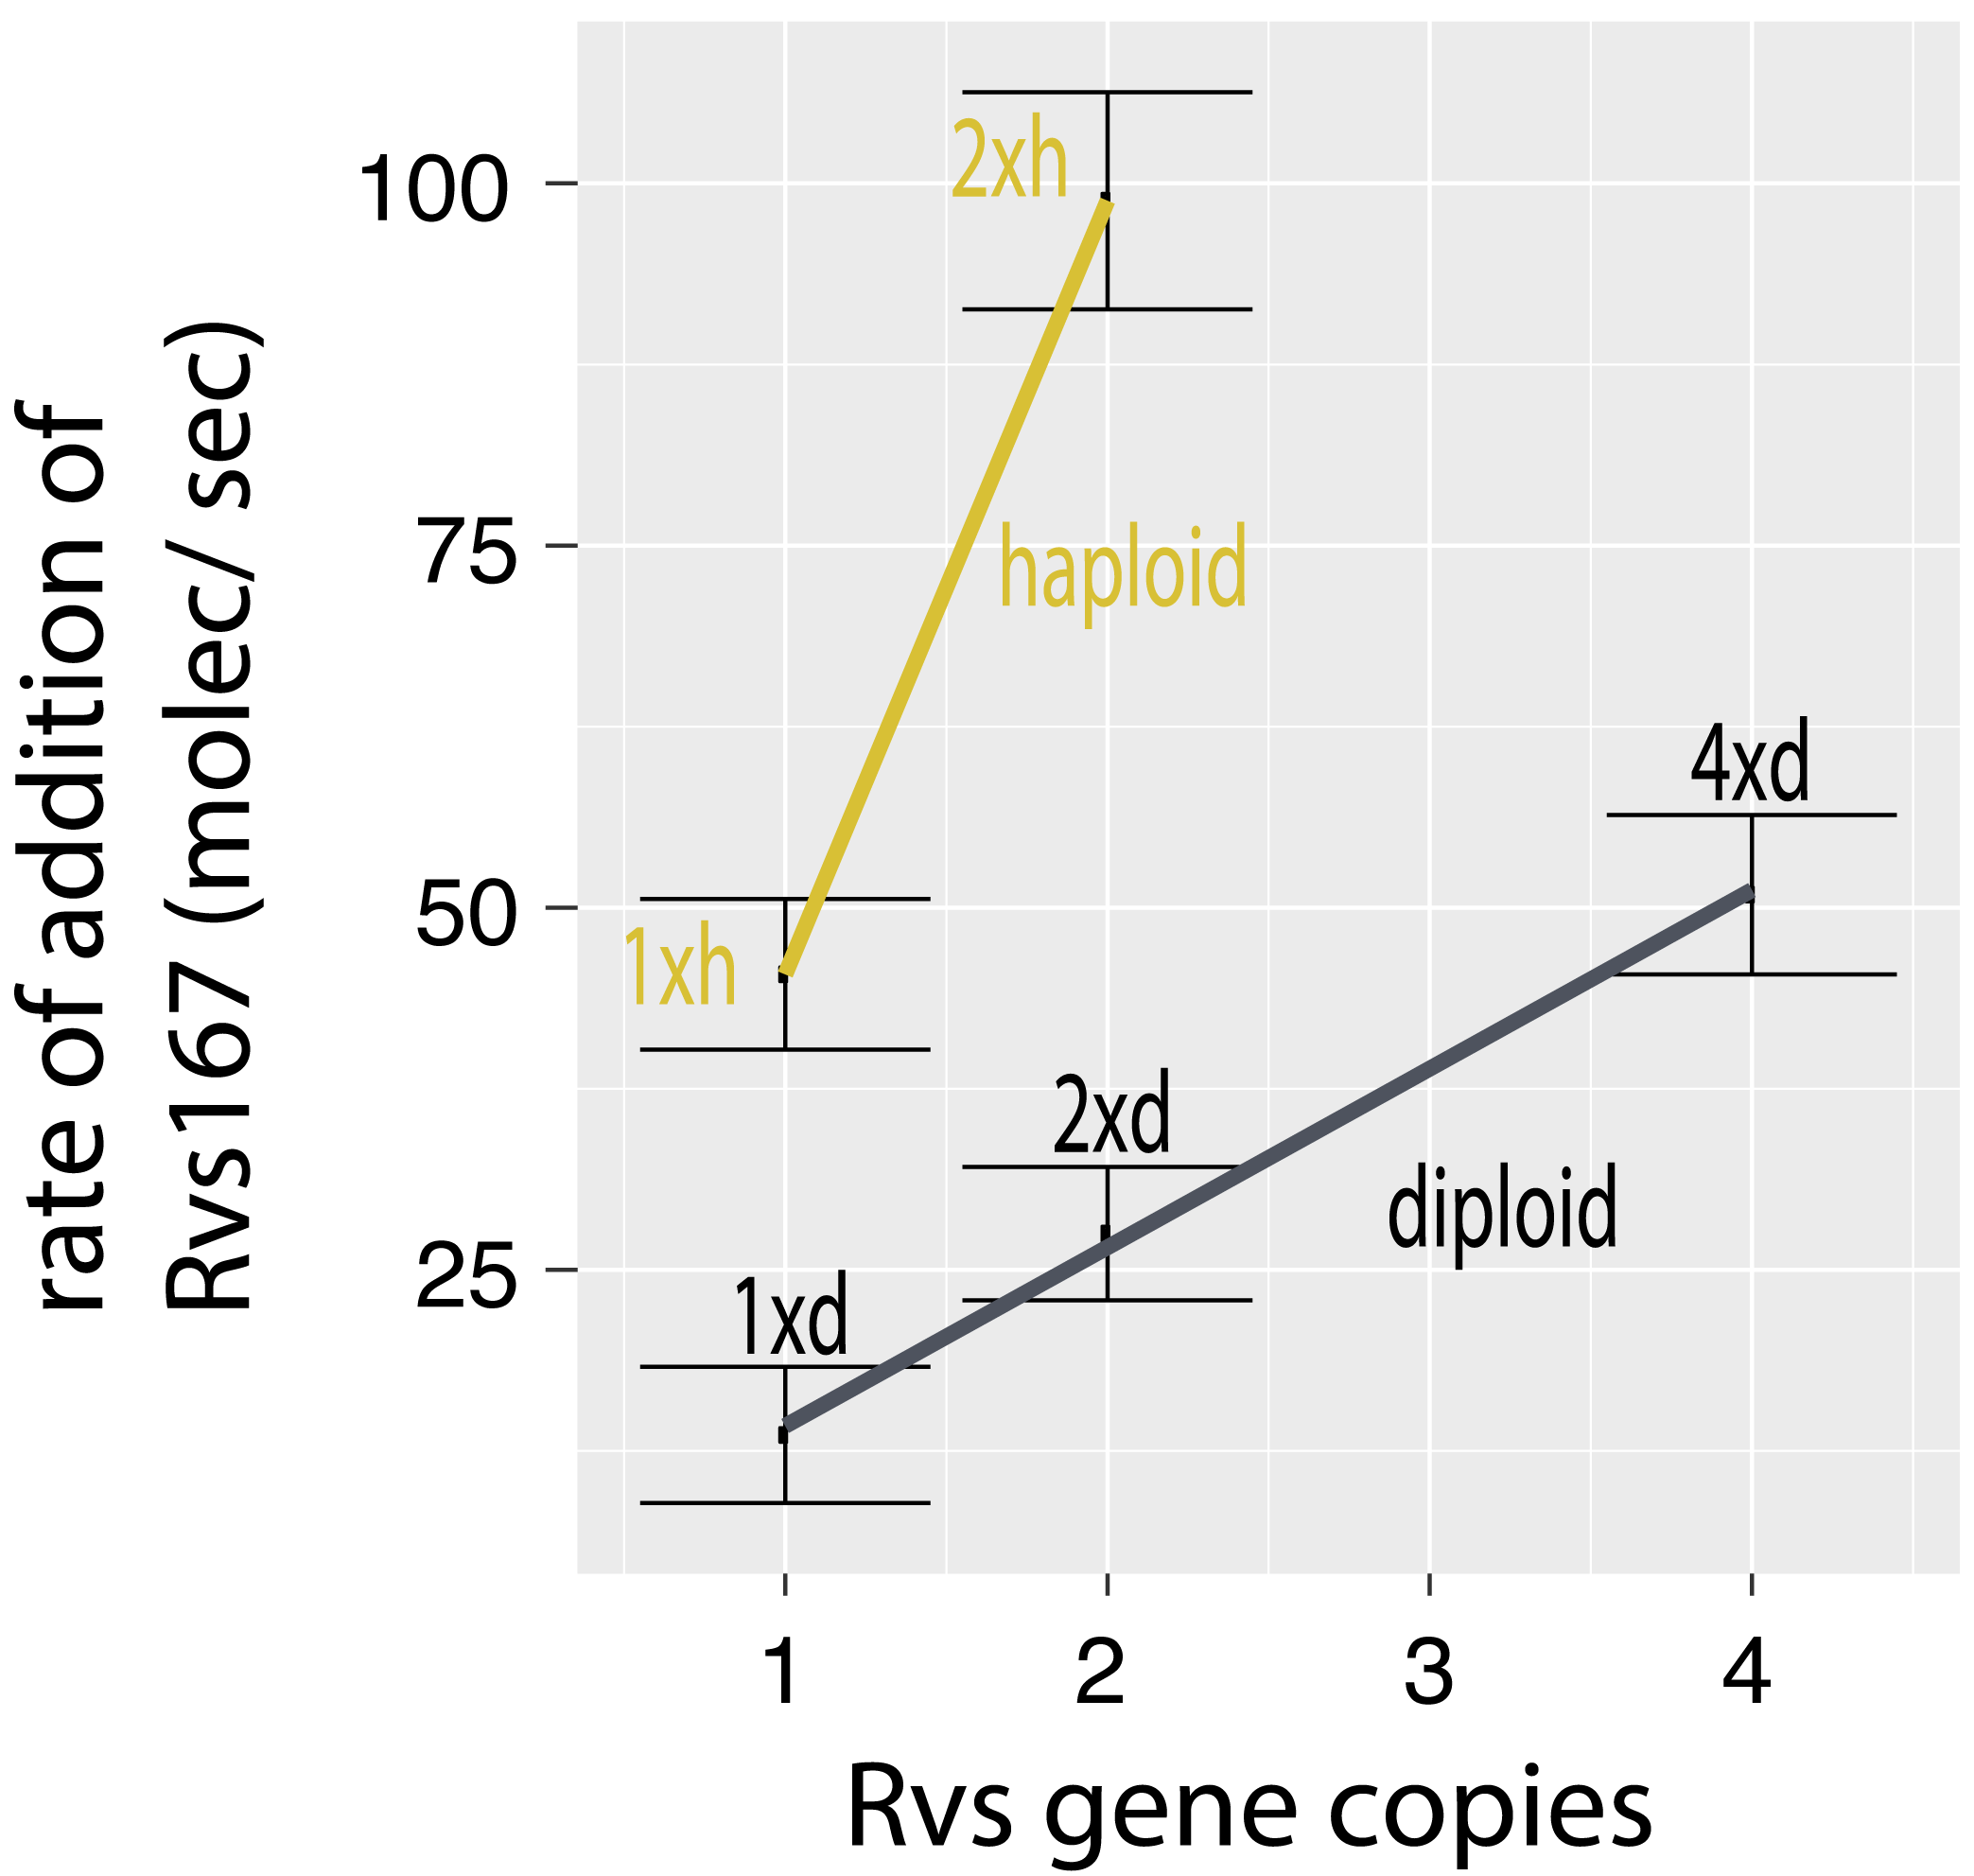
\includegraphics[width=7cm,height=7cm,keepaspectratio]{figures/discussion/recruit_rate_final}
	\caption[Rate of recruitment of Rvs]
{Rate of Rvs molecules added to endocytic sites vs. gene copy number in haploids and diploids. Standard error of mean of the molecule numbers recruited, and linear fit through the data is shown.
	\label{disc_recruit_rate}}
\end{figure}

	\vspace{5mm}
Cytoplasmic protein concentration is increased when gene copy number is  increased, and recruitment to endocytic sites is increased by the increase in cytoplasmic concentration. These data suggest that the amount of Rvs that is recruited scales with available concentration of protein. Comparing across ploidy however, the rate of Rvs recruitment is lower in WT diploid compared to WT haploid (2xd vs 1xh, Fig.\ref{disc_conc}) in spite of the same cytosolic concentration of Rvs in both. The reason for this is not clear. 


%	\vspace{5mm}
%Cytoplasmic protein concentration is increased when gene copies are increased, and recruitment to endocytic sites is increased by the increase in cytoplasmic concentration. Although this data needs to be confirmed by quantitative western blots for protein expression, it suggests that how much Rvs is recruited scales with available concentration of protein. 



\section{Arrangement of Rvs dimers on the membrane}
A homology model of the Rvs BAR dimer structure based on Amphiphysin suggests that it has the concave structure typical for N-BAR domains. Rvs is a hetero- rather than homodimer unlike Amphiphysin, and a high-resolution structure will be necessary to clarify the interaction and arrangement of Rvs on endocytic tubes. There are some indications from the experiments in this thesis however, regarding its interaction with the membrane.



\subsection{Rvs does not form a tight scaffold on membrane tubes}
\textit{In vitro} helices of BAR domains have suggested that Rvs might form a similar helical scaffold. The number of Rvs molecules recruited to endocytic sites is high enough to cover the surface area of the tubular invagination, so it has been proposed that an Rvs scaffold covers the entire membrane tube up to the base of the future vesicle (Picco et al., 2015). 

	\vspace{5mm}
In Rvs duplicated diploid cells (4xd), Rvs can be recruited at a much faster rate than in the WT (2xd) (Fig.\ref{fig_rvsdiploid1}B-C, Fig.\ref{disc_recruit_rate}) while disassembly dynamics is the same in both (Fig.\ref{fig_rvsdiploid1}C, Fig.\ref{decay_final}). The exponential decay of fluorescent intensity in WT haploid and diploid cells (1xh, 2xd, Fig.\ref{decay_final}) indicates that all of the protein is suddenly disassembled from the endocytic site. When the membrane tube undergoes scission, there is no more tubular curvature for the Rvs to bind to. The sharp decay is therefore consistent with a BAR scaffold that breaks upon vesicle scission because there is no more membrane interaction, releasing all the membrane-bound protein at once. 



	\vspace{5mm}
A similar decay in the 4xd strain suggests that all the Rvs in this case is also bound to the membrane: if the protein was not bound to the membrane, fluorescent intensity would not decay sharply. Since the membrane is able to accommodate 1.4x the amount of BAR protein as the WT, it would suggest that at lower protein amounts, a tight helix that covers the entire tube is not likely. Adding molecules to a tube already completely covered by a scaffold would result in a change in Rvs assembly and disassembly dynamics. 

	\vspace{5mm}
Further, additional molecules would have to be added at the top or base of a tight scaffold. At the top, the radius of curvature is decreased compared to the tube since this is the rounded vesicle region. At the base, the plasma membrane is nearly flat, and the Rvs BAR domain is similarly unlikely to favour interactions here. Otherwise the scaffold would have to be disrupted to add new molecules, which would likely slow down recruitment rate rather than speed it up. Molecules could also be added concentric to an existing scaffold. However, the concave surface of Rvs is known to interact with lipids, and multiple layers of BAR domains on the membrane tube would probably not show the sudden disassembly seen here.  

	\vspace{5mm}
I assume that the membrane surface area does not change in the 4xd compared to 2xd from the identical movement of Sla1 in both cases (Fig.\ref{fig_rvsdiploid1}A). It is possible that a wider tube is formed, which would increase the membrane surface area for BAR binding. This would, however, require the BAR domains to interact with a lower radius of curvature than in WT. This seems unlikely, and in the absence of any indication otherwise, I assume that the membrane tubes in all diploid and haploid cases have the same width.


\subsection{A limit for how much Rvs can be recruited to the membrane}
In the case of Rvs duplication in haploids (2xh), a change in disassembly dynamics is seen (Fig.\ref{fig_rvshaploid}C, Fig.\ref{decay_final}). In 2xh, the maximum number of molecules recruited is 178$\pm$7.5 compared to the maximum of 113.505$\pm$5.2 in WT (1xh). This is means that nearly 1.6x the WT amount of protein is recruited to membrane tubes in in the 2xh case. The Rvs167 fluorescent intensity in 2xh shows a delay in disassembly. This suggests that the excess protein may not be directly on the membrane, since if the protein was membrane bound, when the membrane breaks, the protein must be released. The excess Rvs could either interact with the actin network via the SH3 domain, or interact with other Rvs dimers. By a similar argument as in 4.2.1 above, I do not expect that multiple layers of BAR domains are formed, and that the excess protein is recruited by the interaction of the SH3 domain. 


	\vspace{5mm}
Another explanation for the delayed disassembly is that at high concentrations of Rvs like in the 2xh case, a tight BAR scaffold is formed, and the BAR domains interact with adjacent BAR domains. When the membrane undergoes scission, the protein is no longer membrane-bound, but lateral interactions delay disassembly of the scaffold. Lateral interactions between neighbouring BAR dimers have been shown in the case of Endophilin (Mim et al., 2012). It is not currently clear where the Rvs molecules are added in the 2xh case: supperresolution microscopy could clarify whether it is added at the membrane tube.

\vspace{5mm}
Whatever the arrangement of the Rvs complex on the membrane, disassembly dynamics is changed in the case of 2xh, compared to the other haploid and diploid strains. Since the number of Rvs molecules is highest in this strain, this suggests that there is a limit to how much Rvs can assemble on the tube without altering interaction with the endocytic protein network. 

\begin{figure}[H]
	\centering
	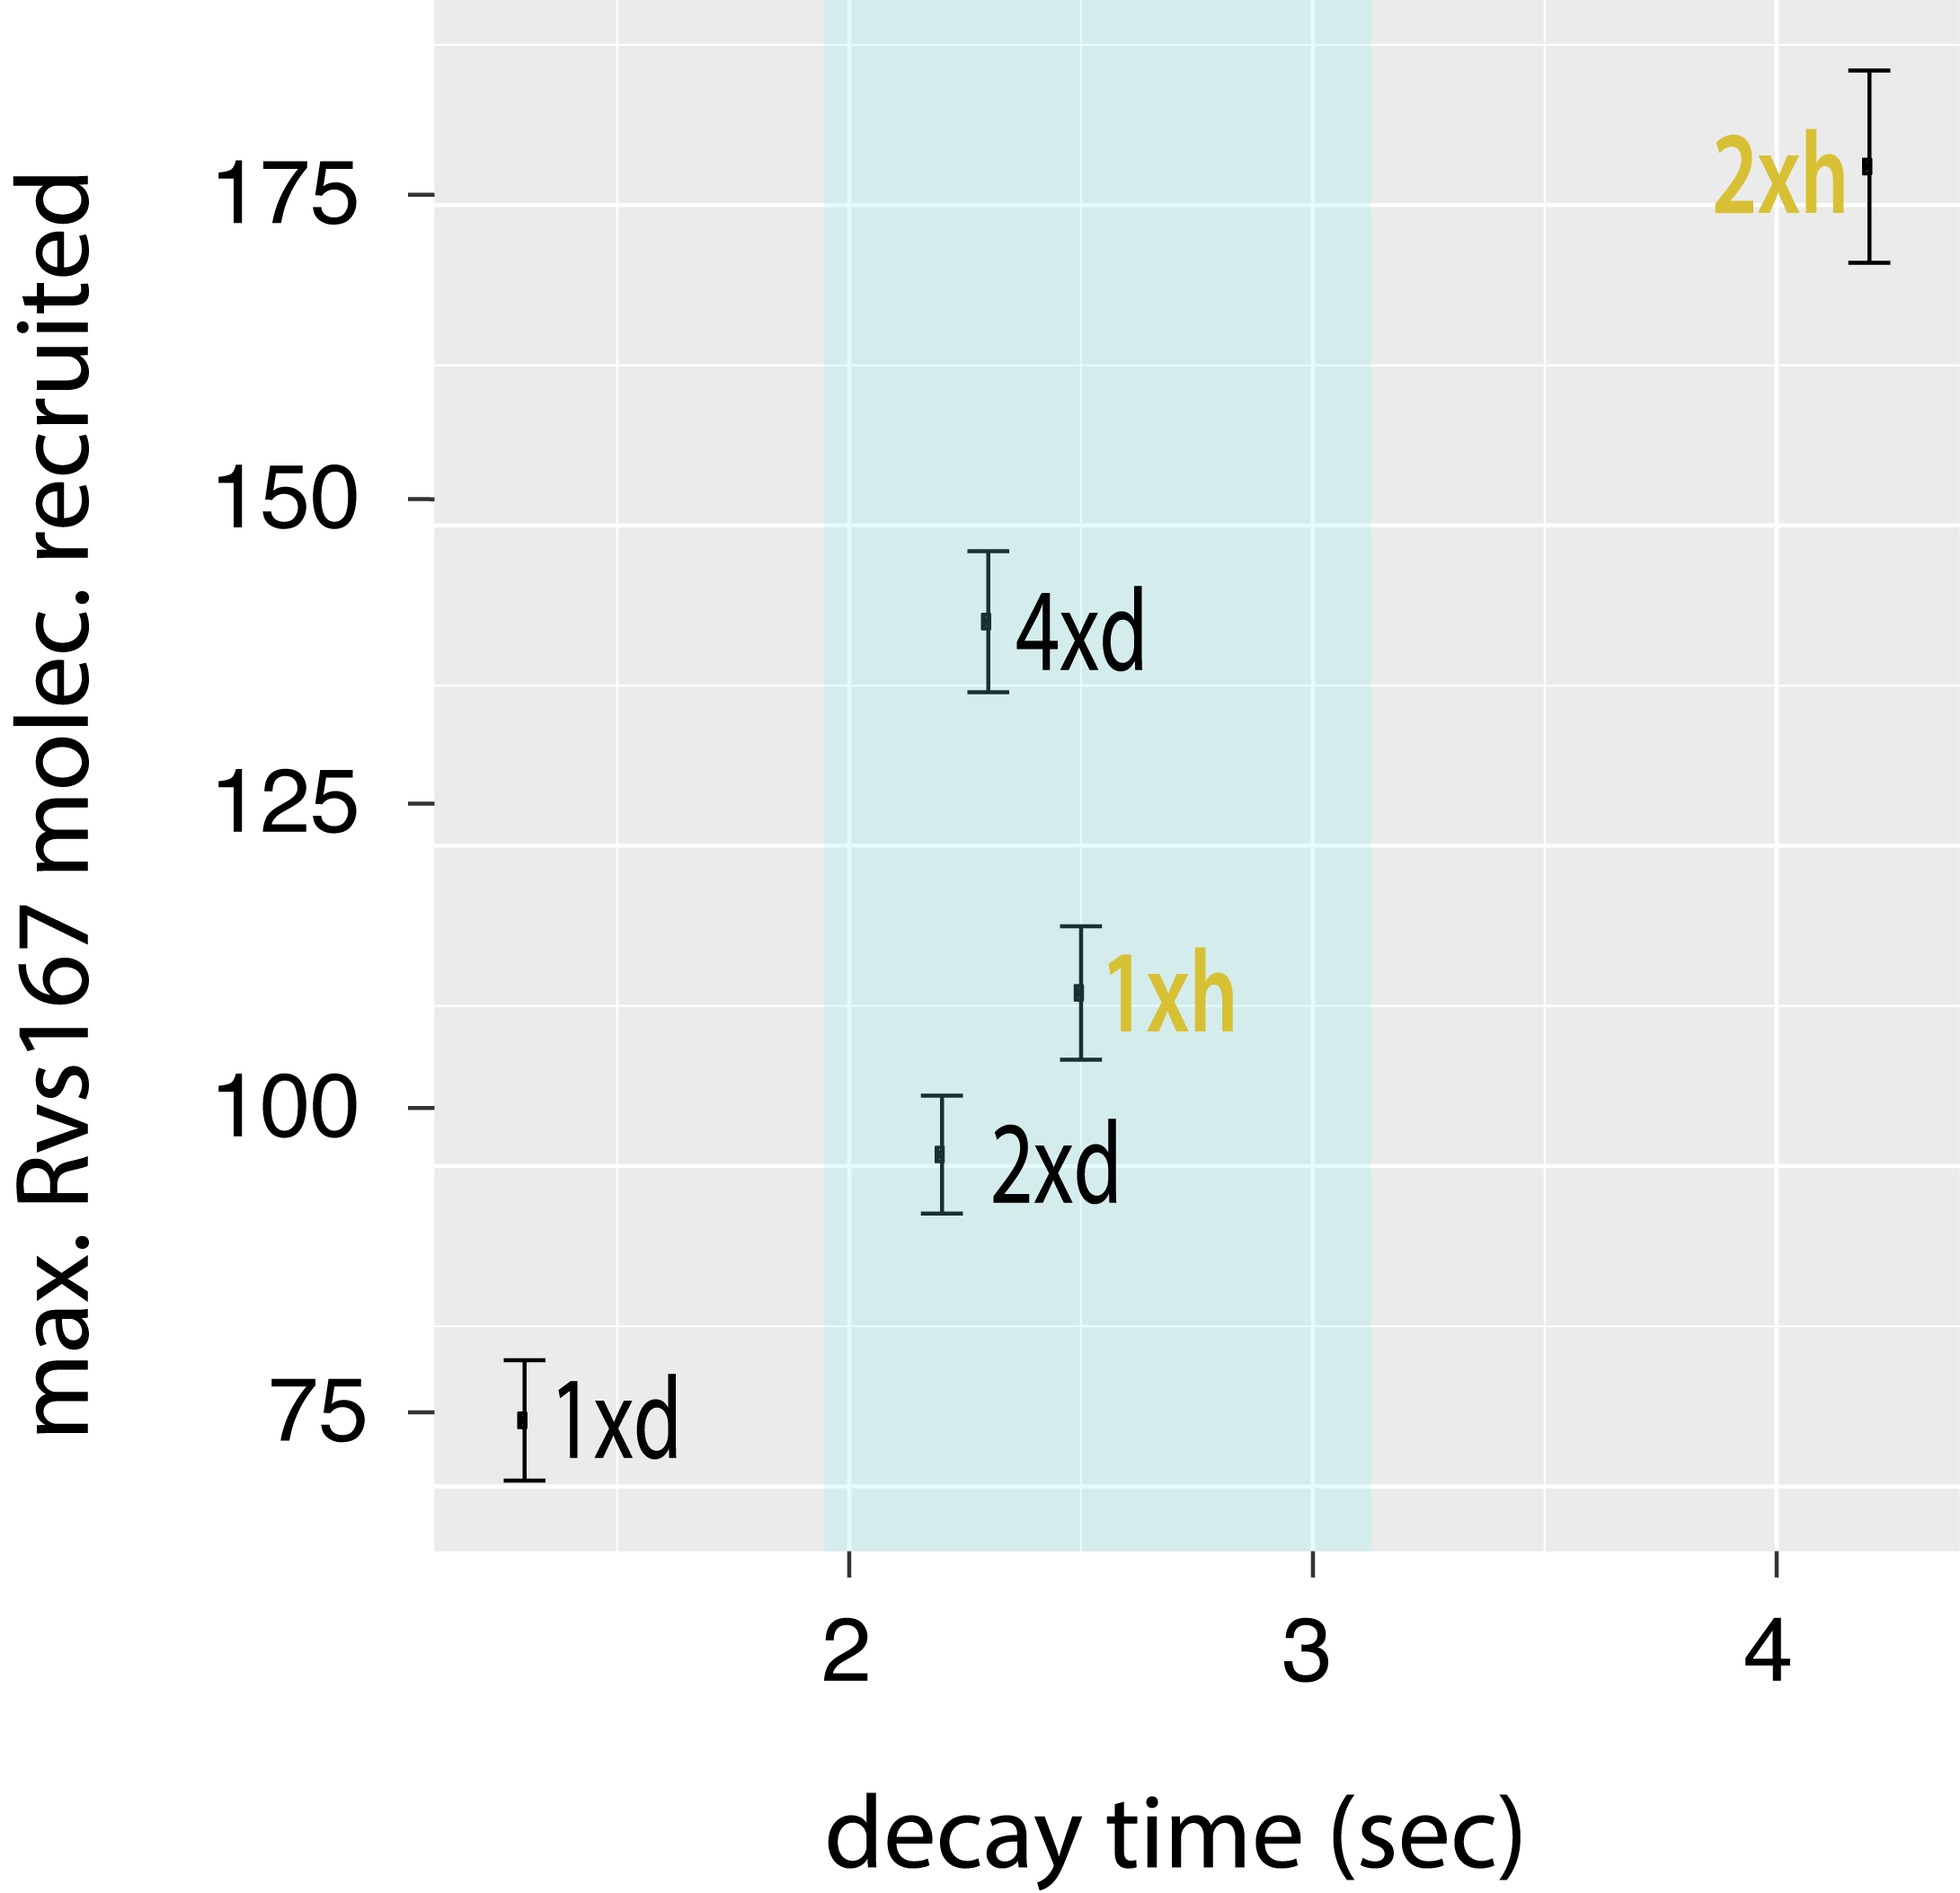
\includegraphics[width=8cm,height=8cm,keepaspectratio]{figures/discussion/decay_final}
	\caption[Rvs decay time]
	{Time from peak of Rvs167 fluorescent intensity to minimum intensity, against maximum molecule numbers recruited. Coloured region highlights similar disassembly time for increasing amounts of molecules recruited.    
		\label{decay_final}}
\end{figure}

\subsection{Conclusions for Rvs localization }
All of these data support the idea that Rvs recruitment rate and total numbers are determined by concentration of protein in the cell. The maximum number of molecules that can interact with the membrane is limited by the surface area of the invagination. Although more can be recruited, Rvs molecules over a certain threshold interact in a different way with endocytic sites, possibly via the SH3 domain. Timing of recruitment to sites is by curvature-recognition via the BAR domain, while efficiency of recruitment and interaction with the actin network is established via the SH3 domain. 



\section{What causes membrane scission?}


\subsection{Dynamin does not not drive scission}
Some studies have suggested that dynamin-like Vps1 localizes to endoytic sites, and affects the scission mechanism: Nannapaneni et al (Nannapaneni et al., 2010)., find that the lifetimes of Las17, Sla1, Abp1 increase in the absence of Vps1. Rooij et al (Rooij et al., 2010)., find that Rvs167 lifetimes increase, and are recruited in fewer patches to the cell cortex. On the other hand, \textit{vps1$\Delta$} did not increase the scission failure rate of \textit{rvs167$\Delta$} in other studies (Kishimoto et al., 2011), and did not co-localize with endocytic proteins (Goud Gadila et al., 2017). If Vps1 was to affect scission, the number of failed scission events should increase in \textit{vps1$\Delta$} cells, but I do not find so, confirming other studies (Kishimoto et al., 2011). Vps1 tagged with GFP and imaged in TIRF does not form cortical patches that co-localize with Abp1-mCherry (data from Andrea Picco, not shown). GFP-tagging could affect the recruitment of Vps1 to endocytic sites while maintaining its role in other pathways of vesicular trafficking. Membrane movement and scission dynamics are however, unchanged in the absence of Vps1. If loss of Vps1 prevented or delayed scission, the membrane would continue to invaginate longer than WT lengths, and Sla1 movements of over 140nm should be observed. Rvs centroid movement would likely also be affected: a bigger jump inwards could indicate that that a longer membrane has been cut. My observation that there are no changes in the behaviour of coat and scission markers indicates that even if Vps1 is recruited to endocytic sites, it is not necessary for Rvs localization or function, and is not necessary for scission. 



\subsection{Lipid hydrolysis is not the primary cause of membrane scission}
In this model, synaptojanins hydrolyze 	PIP\textsubscript{2} that are not covered by BAR domains, resulting in a boundary between hydrolyzed and non-hydroplyzed 	PIP\textsubscript{2} The model predicts that interfacial forces generated at the lipid boundary causes scission (Liu et al., 2006).  Inp51 is not seen in patches at the cellular cortex, but this could be because protein recruitment is below our detection threshold. Inp52 localizes to the top of invaginations right before scission, consistent with a role in vesicle formation (Fig.\ref{fig_inp}D). Some predictions of the lipid hydrolysis model are inconsistent with our data, however. 


\vspace{5mm}

First, vesicle scission is expected to occur at the interphase of the hydrolyzed and non-hydrolyzed lipid. Since the BAR scaffold covers the membrane tube, this interphase would be at the top of the area covered by Rvs. Kukulski et al., 2012 have shown that vesicles undergo scission at 1/3 the invagination length from the base: that is, vesicles generated by the lipid boundary would be smaller than have been measured. Second, removing forces generated by lipid hydrolysis by deleting synaptojanins should increase invagination lengths, since scission would be delayed or it would fail without those forces. Deletion of neither Inp51 nor Inp52 changes the invagination lengths: Sla1 movement does not increase. That the position of the vesicle formed is also unchanged compared to WT is indicated by the similar magnitude of the jump into the cytoplasm of the Rvs centroid. 


\vspace{5mm}
There are some changes in the synaptojanin deletion strains (Fig.\ref{fig_inpmov}). In \textit{inp51$\Delta$} cells, Rvs assembly is slightly slower than that in WT. Therefore, Inp51 could play a role in Rvs recruitment. In the \textit{inp52$\Delta$} strain, about 12\% of Sla1-GFP tracks retract, indicated that scission fails in those cases. Although this is low compared to the failed scission rate of \textit{rvs167$\Delta$} cells (close to 30\%), this data could suggest a moderate influence of Inp52 on scission. Rvs centroid persists after scission for about a second longer in \textit{inp52$\Delta$} cells than in WT, indicating that disassembly of Rvs on the base of the newly formed vesicle is delayed.

\vspace{5mm}
In \textit{inp51$\Delta$}\textit{inp52$\Delta$} cells, Rvs is accumulated at patches, but majority of Rvs patches do not show the typical sharp jump into the cytoplasm. Membrane morphology is hugely aberrant in these cells, complicating interpretation of this data (Srinivasan et al., 1997). Electron microscopy shows long, undulating membrane invaginations (Srinivasan et al., 1997). Fluorescence microscopy shows that multiple endocytic sites that are assembled and disassembled at these long invaginations, and fail to undergo scission (Sun et al., 2007). Where on these long membranes Rvs localizes could be clarified by CLEM or super-resolution microscopy. Large clusters of Rvs seen in the \textit{inp51$\Delta$}\textit{inp52$\Delta$} strain could be multiple Rvs patches on same membrane tube. Pooling signal from multiple endocytic sites would influence the molecule numbers acquired by our analysis, and yield a higher number than at a single site. Rvs does, interestingly, assemble and disassemble in these mutants. If no vesicles are formed at these membranes, it would indicate that Rvs disassembly is not caused by membrane scission.


\subsection{Protein friction does not drive membrane scission}
Protein-friction mediated membrane scission proposes that BAR domains induce a frictional force on the membrane, causing scission. In Rvs duplicated haploid cells (2xh), adding up to 1.6x the WT (1xh) amount of Rvs to membrane tubes does not affect the length at which the membrane undergoes scission (Fig.\ref{fig_rvshaploid}). The model introduced in Section\ref{friction_model} predicts that if more BAR domains were added to the membrane tube, frictional force generated as the membrane is pulled under it will increase, and the membrane would rupture faster. That is, membrane scission occurs as soon as WT forces are generated on the tube. Since BAR domains are added at a faster rate in the 2xh cells, these forces would be reached at shorter invagination lengths. In 2xh cells, WT amount of Rvs is recruited at about 1.8 seconds before maximum fluorescent intensity, but scission does not occur at this time. Instead, Rvs continues to accumulate, and the invagination continues to grow. In diploid strains, adding 1.4x the WT amount of Rvs in the 4x Rvs case also does not change length of membrane that undergoes scission. Therefore, protein friction due to Rvs does not appear to contribute significantly to membrane scission in yeast endocytosis. 


\subsection{ Actin polymerization generates forces required for membrane scission}
Maximum amount of Abp1 measured in all the diploid strains is about 220 molecules (Fig.\ref{fig_rvsdiploid2}). In this case, only one allele of Abp1 is fluorescently tagged, so half the amount of Abp1 recruited is measured. The maximum amount of Abp1 recruited is then double that measured, which is about 440$\pm$20 molecules (assuming equal expression and recruitment of tagged and untagged Abp1). In WT haploid cells, the maximum number of Abp1 measured is 460$\pm$20 molecules. That the same number of molecules of Abp1 is recruited in all cases before scission indicates that scission timing depends on the amount of Abp1, and hence, on the amount of actin recruited. 

\vspace{5mm}
This data is consistent with actin supplying the forces necessary for membrane scission. The membrane invagination continues until the “right” amount of actin is recruited. At this amount of actin, enough forces are generated to rupture the membrane. The amount of force necessary is determined by the physical properties of the membrane like membrane rigidity, tension, and proteins accumulated on the membrane (Dmitrieff and Nédélec, 2015). Vesicle scission releases membrane-bound Rvs, resulting in release of the SH3 along with BAR domains. Release of the SH3 domains could indicate to its binding partner in the actin network that vesicle scission has occurred, beginning disassembly of actin components. In BAR strains, a low amount of actin is recruited (Fig.\ref{fig2_sh3del}C). Although the absence of the SH3 domain severely perturbs the actin network, the mechanistic effect of this perturbation is unclear. 

\section{Function of the Rvs complex}

\subsection{Rvs scaffolds the membrane tube}
Invaginations in \textit{rvs167$\Delta$} cells undergo scission at short invagination lengths of about 80nm (Fig.\ref{fig2_rvsdelta}), compared to the WT lengths of 140nm. This shows that first, enough forces are generated at 80nm to cause scission. Then, that Rvs167 is required at membrane tubes to prevent premature scission. 

\vspace{5mm}
Prevention of scission at short invagination lengths can be explained by Rvs stabilizing the membrane invagination via membrane interactions of the BAR domain (Boucrot et al., 2012; Dmitrieff and Nédélec, 2015). Rvs preventing membrane scission could also be explained by the SH3 domain mediating actin forces to the invagination neck: one can imagine that the SH3 domain somehow decouples actin forces from the neck, and that this delays scission. Since invagination lengths of \textit{rvs167$\Delta$} cells are increased towards WT by overexpression of the BAR domain alone (Fig.\ref{fig_scaffold}A), I propose that localization of Rvs BAR domains to the membrane tube stabilizes the membrane. This allows deep invaginations to grow until actin polymerization produces enough forces to overcome this stabilization and sever the membrane. Stabilization of the membrane tube increases with increasing amounts of BAR domains recruited to the membrane tube (Fig.\ref{fig_scaffold}). The requirement for Rvs scaffolding cannot be removed by reducing turgor pressure (Fig.\ref{fig_sorbitol}), suggesting that the function of the scaffold is not to counter turgor pressure. 

%\subparagraph{Role of the N-terminal helix}
%The N-terminal amphiphatic helix has been shown to oppose the stabilizing effect of BAR domains by inducing membrane scission via shallow insertions of the helix into the membrane bilayer. The shallow insertions induce scission in a concentration dependent manner. In the case of yeast scission, since increasing the concentration of Rvs does not speed up the scission process, I do not expect that the N-helix plays a role in vesicle formation. The N-helix has also been shown to reqiured for membrane interaction, and could help the recruitment of Rvs to endocytic sites. The effect of the N-helix is currently being invesitaged.

\subsection{A critical amount of Rvs is required to stabilize the membrane }

%\vspace{5mm}
Scission efficiency decreases with decreased amounts of Rvs: in diploids, lowering the amount of Rvs by 20 molecules decreases scission efficiency to about 90\% from 97\% (see Chapter\ref{Ch:Appendix}. This indicates that a particular coverage of the membrane tube is required for effective scaffolding by BAR domains. In support of this, in BAR strains, fewer numbers of Rvs are recruited, and scission efficiency is similarly reduced. At low concentrations of Rvs like in the 1xd cells, it is likeley that some membrane tubes recruit the critical number of Rvs, in which case the invaginations grow to near WT lengths. Over a certain amount of Rvs, adding more BAR domains does not increase the stability of the tube: in 4xd, the same amount of actin is recruited before scission as in the 2xd and 1xd strains. 

	\vspace{5mm}
If enough forces are generated at 80nm, why is scission efficiency decreased in \textit{rvs167$\Delta$} compared to WT? 
Forces from actin may be at a threshold when the invagination is at 80nm. There could be enough force to sever the membrane, but not enough to sever reliably. The Rvs scaffold then keeps the network growing to accumulate enough actin to reliably cause scission. Controlling membrane tube length could also be a way for the cell to control the size of the vesicles formed, and therefore the amount of cargo packed into the vesicle. 





%\section{Role of other scission-stage proteins}
\section{Inp52 is likely involved in vesicle uncoating}
Deletion of synaptojanin-like Inp52 does not affect the movement of the invagination. In spite of this, Sla1 patches persist for longer after scission in the \textit{inp52$\Delta$} than in WT cells, as does Rvs167, indicated by the arrows in Fig.\ref{fig_inpmov}A,D. Persistence of both suggests that rather than the scission timepoint, post-scission disassembly of proteins from the vesicle is inhibited in \textit{inp52$\Delta$} cells. Inp52 then plays a role in recycling endocytic proteins from the vesicle to the plasma membrane. The slower assembly of Rvs in \textit{inp51$\Delta$}  and the increase in coat retraction rates of \textit{inp52$\Delta$} could indicate that there is a slight effect on Rvs recruitment, and that lipid hydrolysis could play a small role in scission. 


\newpage
\section{Model for membrane scisison}
I propose that Rvs is recruited to sites by two distinct mechanisms. SH3 domains cluster Rvs at endocytic sites. SH3 interaction increases the efficiency with which the BAR domain senses curvature on tubular membranes. The BAR domain binds to endocytic sites by sensing tubular membrane. BAR domains are recruited over the entire membrane tube, but do not form a tight helical scaffold. BAR-membrane interactions stabilize the membrane shape against fluctuations that could cause scission. This prevent actin forces from rupturing the membrane, and the invaginations continue to grow in length as actin continues to polymerize and exert forces. 


\begin{figure}[H]
	%	\centering
	\vspace*{1cm}
	\hspace*{-0.cm}
	%	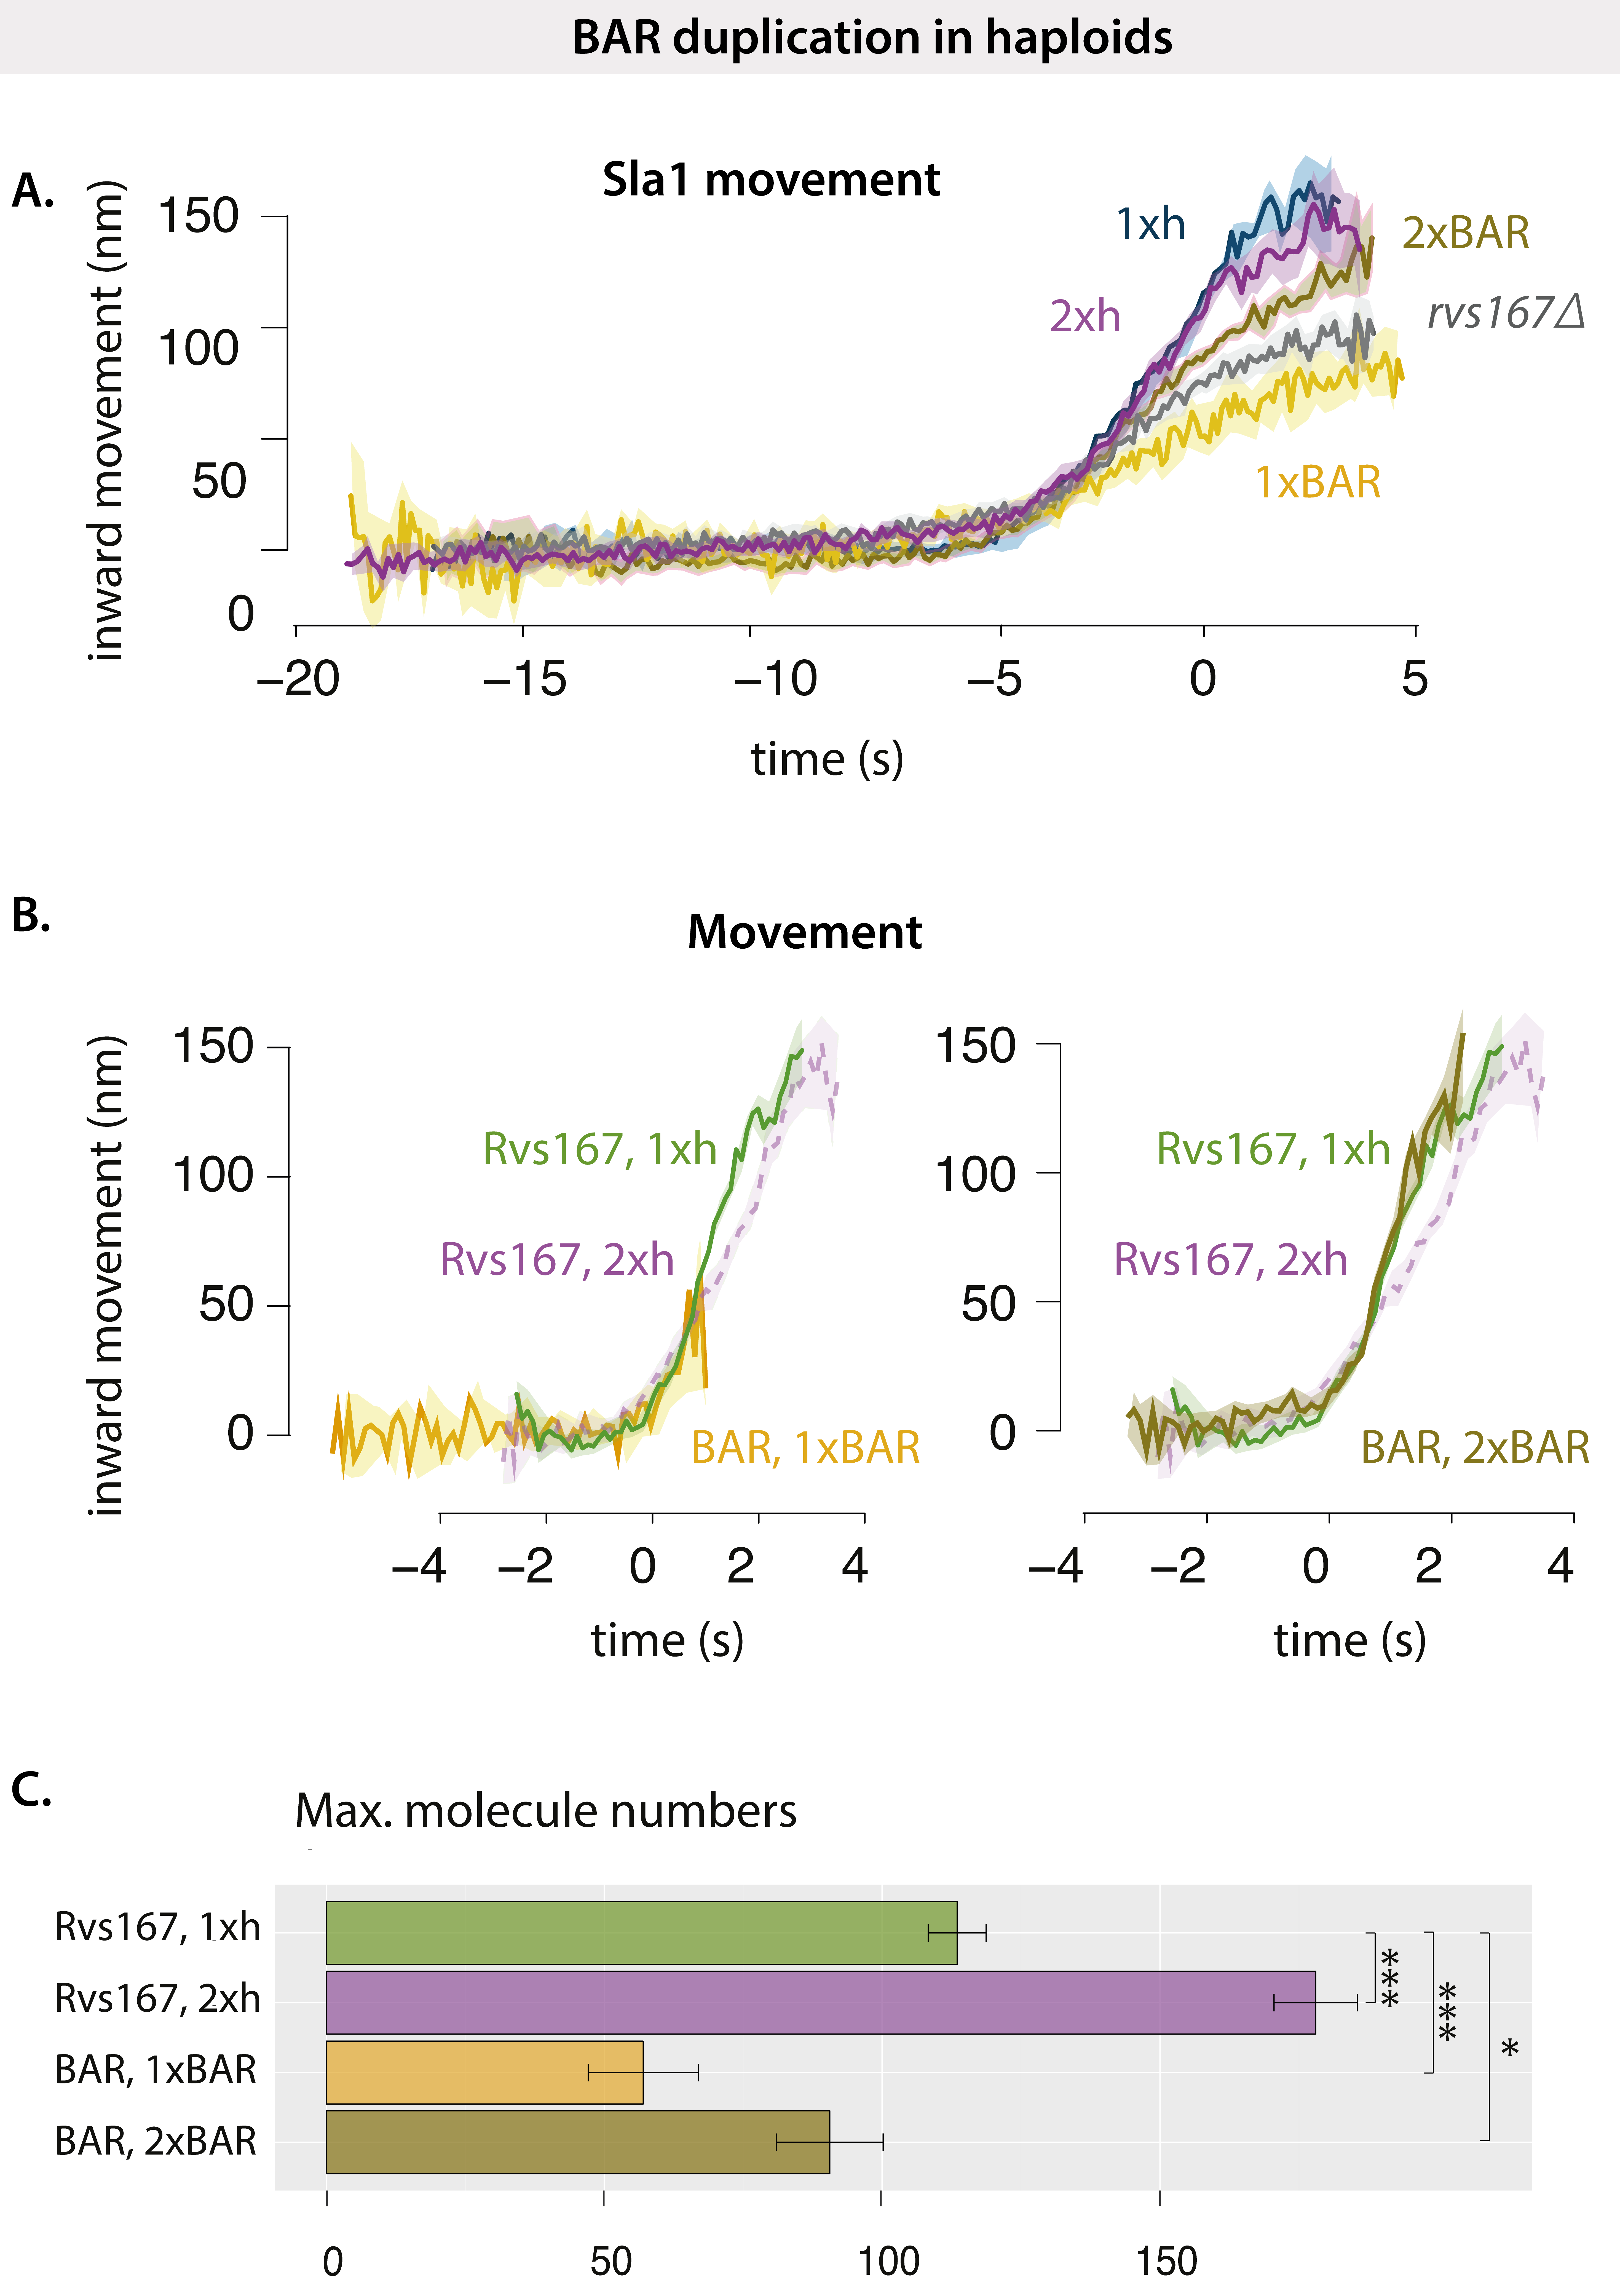
\includegraphics[width=21cm,height=21 cm,keepaspectratio]{figures/results_final/scaffolding_overlaid3}
	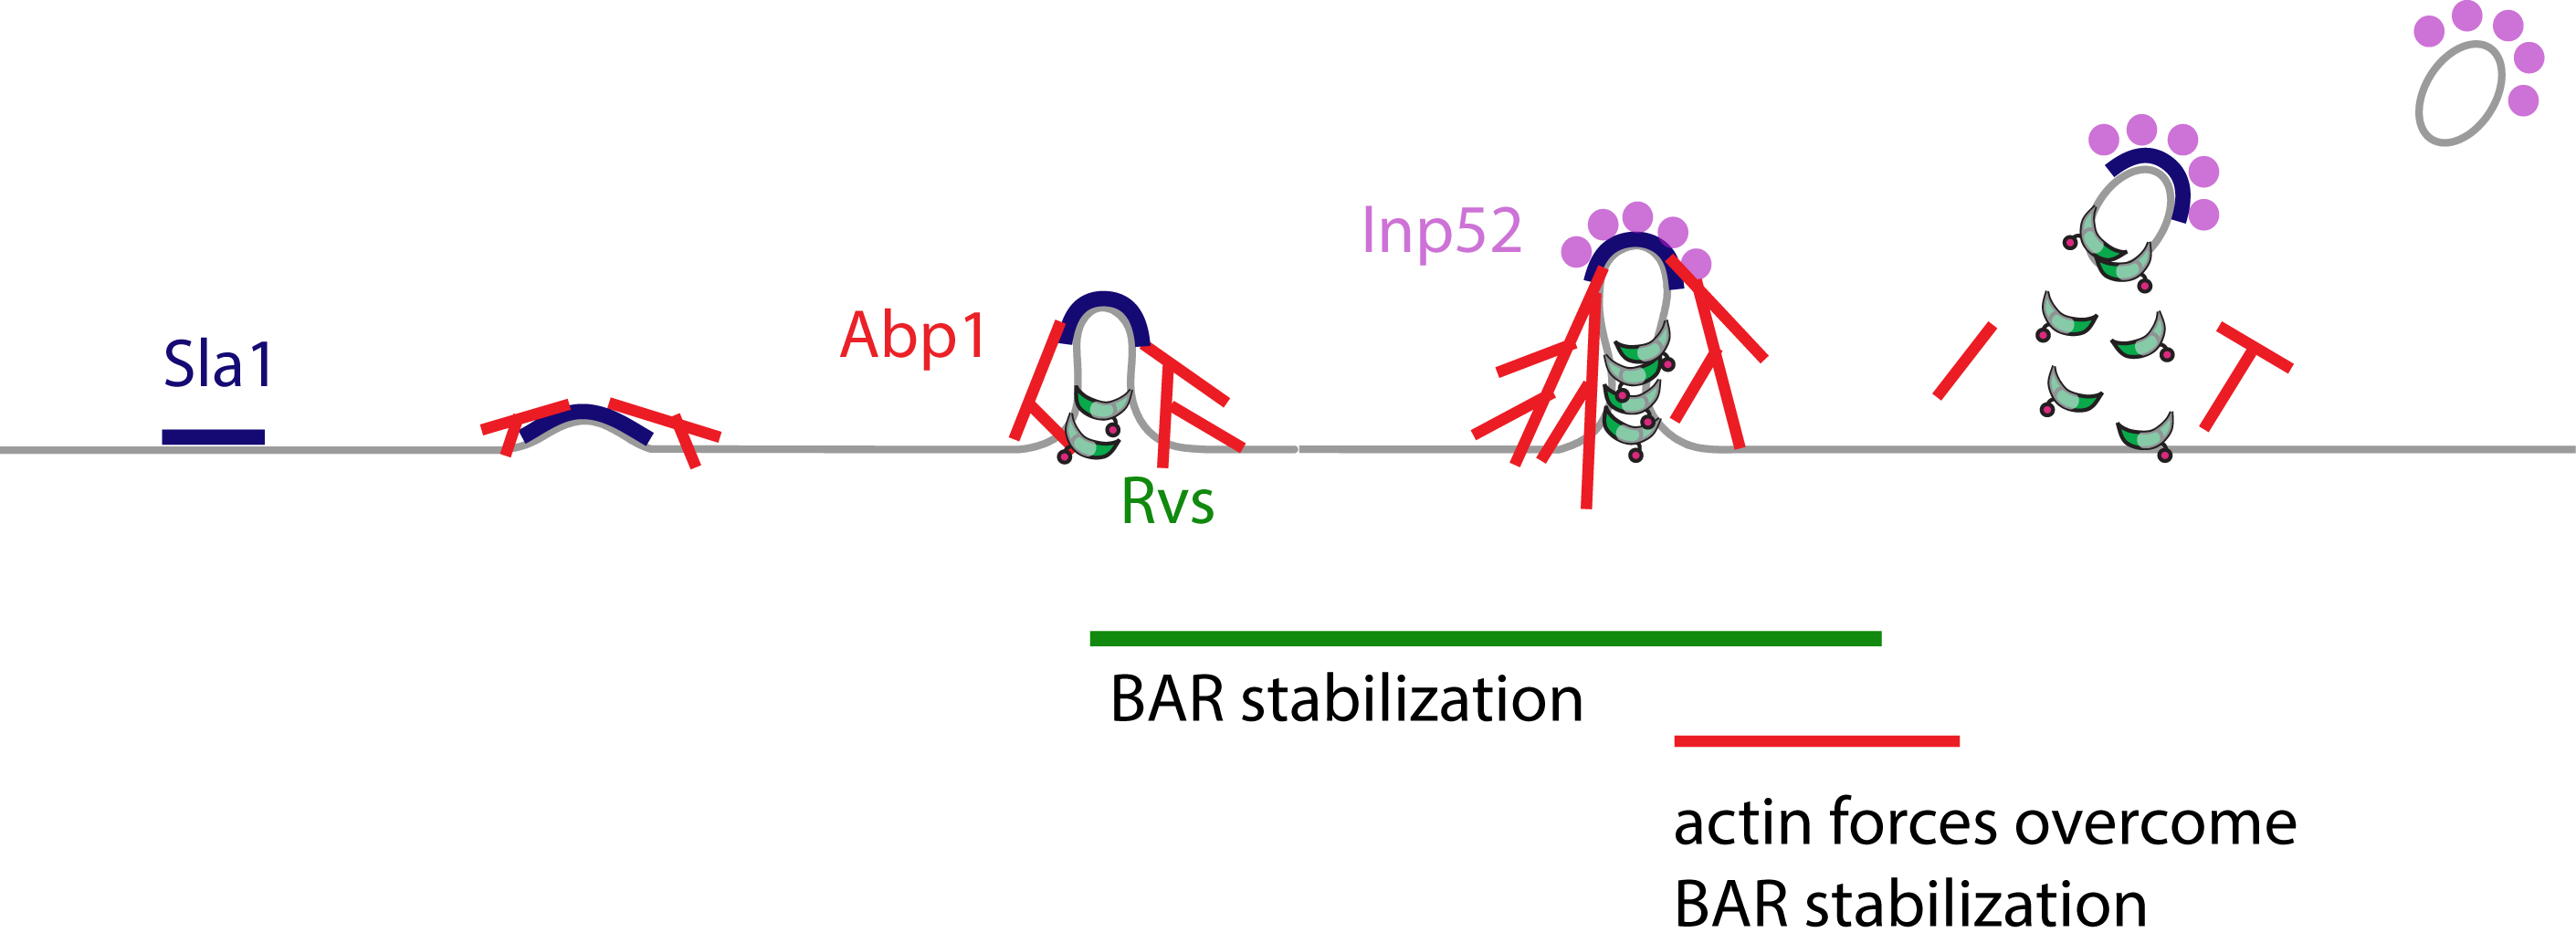
\includegraphics[scale=0.65]{figures/discussion/yeast_schematic_concl2}
	\caption [Model for membrane scission in yeast]
	{ Schematic model for membrane scission in yeast endocytosis. BAR domains are recruited to tubular membranes, and scaffold them, preventing scission. Recruitment to the membrane is increased by the SH3 domain. Actin filaments meanwhile continue to polymerize and eventually exert enough forces to overcome the influence of the BAR scaffold, causing membrane scission. Inp52 is recruited to the top of the invagination right before scission and is involved in uncoating the vesicle. 
		\label{model}}
\end{figure}

BAR recruitment to membrane tubes is restricted by the surface area of the tube: after a certain amount of Rvs, the excess interacts with endocytic sites via the SH3 domain. Adding over a certain amount of Rvs also does not increase the stabilization effect on the tube. As actin continues to polymerize, at a certain amount of actin, enough forces are generated to overcome the resistance to membrane scission provided by the BAR scaffold. The membrane ruptures, and vesicles are formed. Synaptojanins may help recruit Rvs at endocytic sites: Inp51 and Inp52 have proline rich regions that could act as binding sites for Rvs167 SH3 domains. They are involved in vesicle uncoating post-scission, likely by dephosphorylating PIP\textsubscript{2} and inducing disassembly of 	PIP\textsubscript{2}-binding endocytic proteins. Eventually phosphorylation regulation by Ark1/Prk1 allows endocytic proteins to be reused at endocytic sites, while the vesicle is transported elsewhere into the cell. 


%\section{Other potential scission mechanisms and open questions}

%\cite{Dmitrieff2015a}
%clustering induces scission 
%cooperation between lipid hydrolysis and actin forces?


%why these curvatures? specificity from the SH3 domain?
%why does it come off
%regulation of activity? phophorylation/ autoinhibition


\chapter{Materials and Methods} % Main chapter title

\section{Materials} 
\subsection{Yeast strains}
\begin{table}[H]
	\vspace*{-1cm}
	\raggedleft
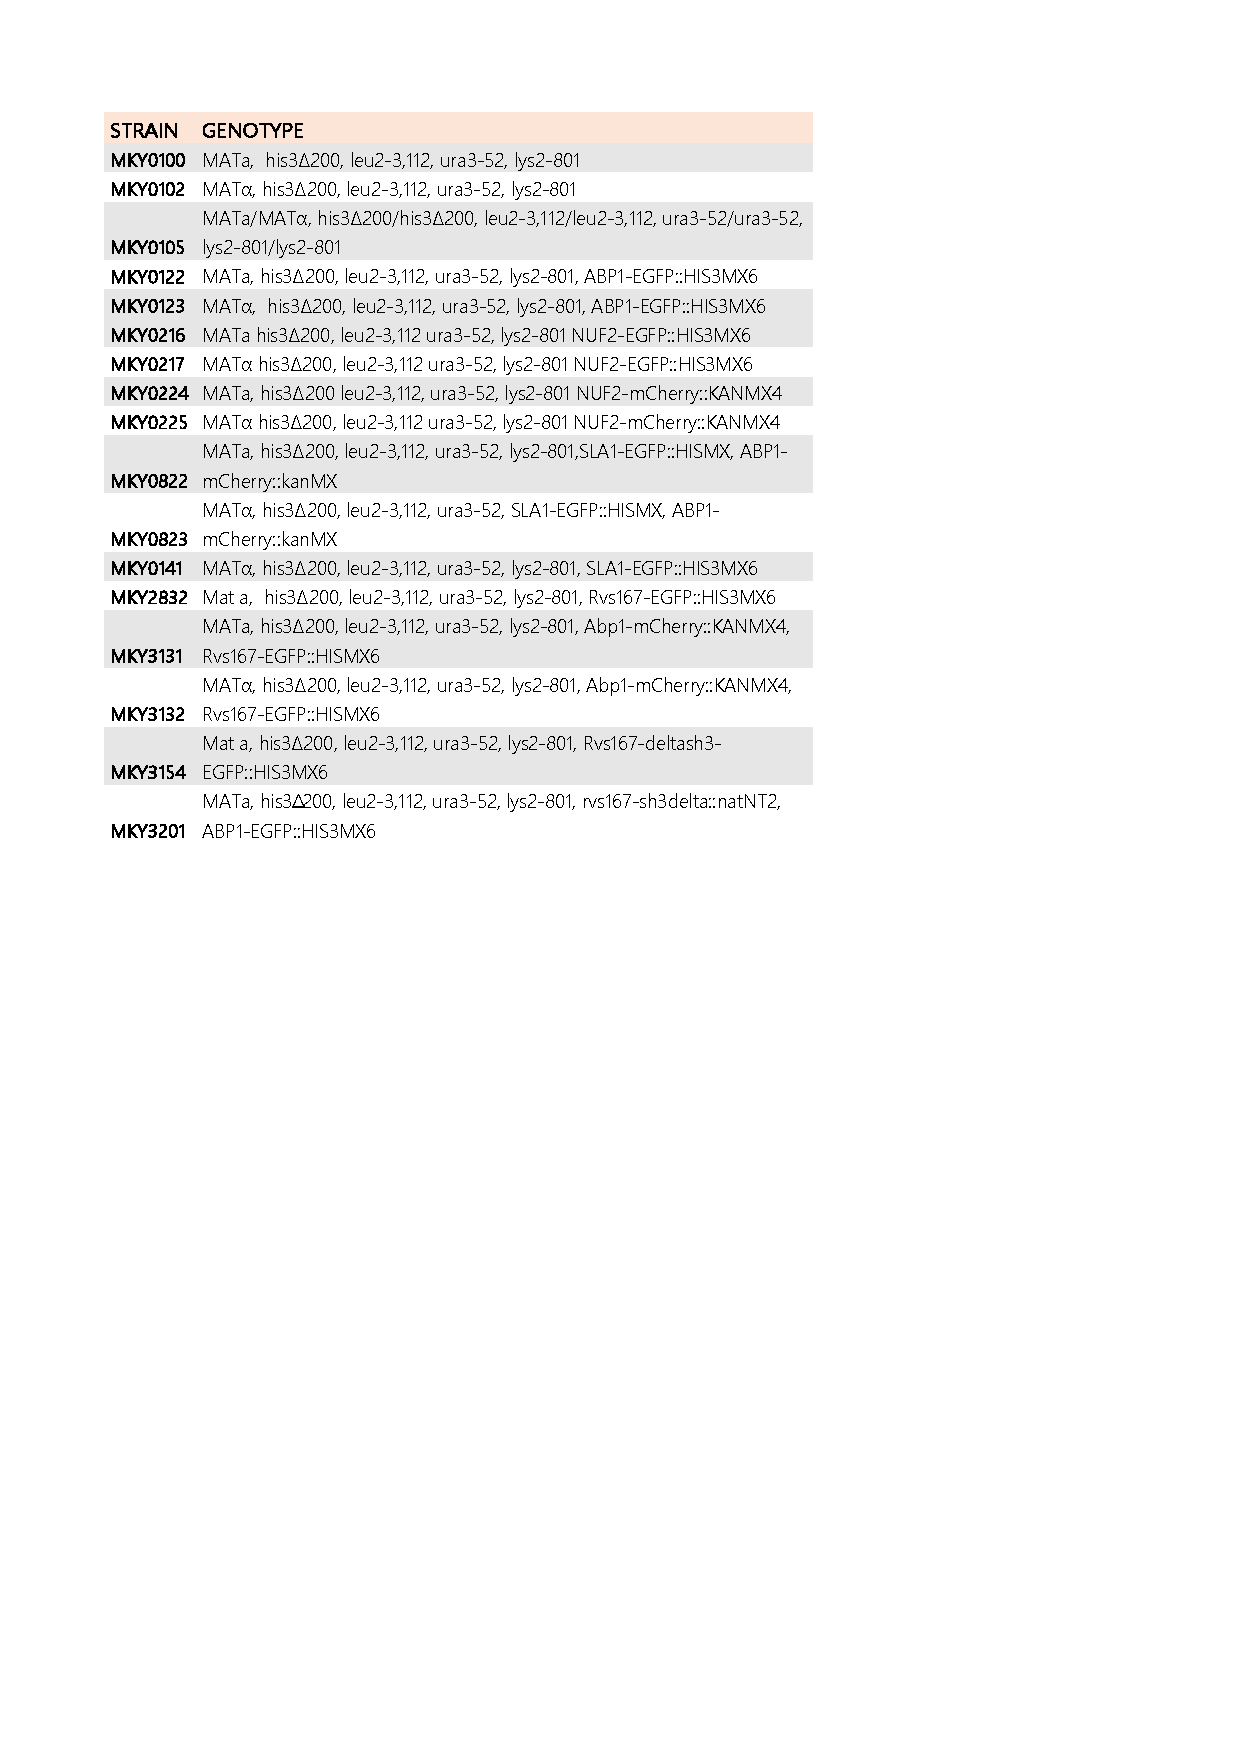
\includegraphics[width=35cm,height=35cm,keepaspectratio, valign=t]{figures/results_final/strains_@1}
\caption[Yeast strains]

\end{table}


\begin{table}[H]
	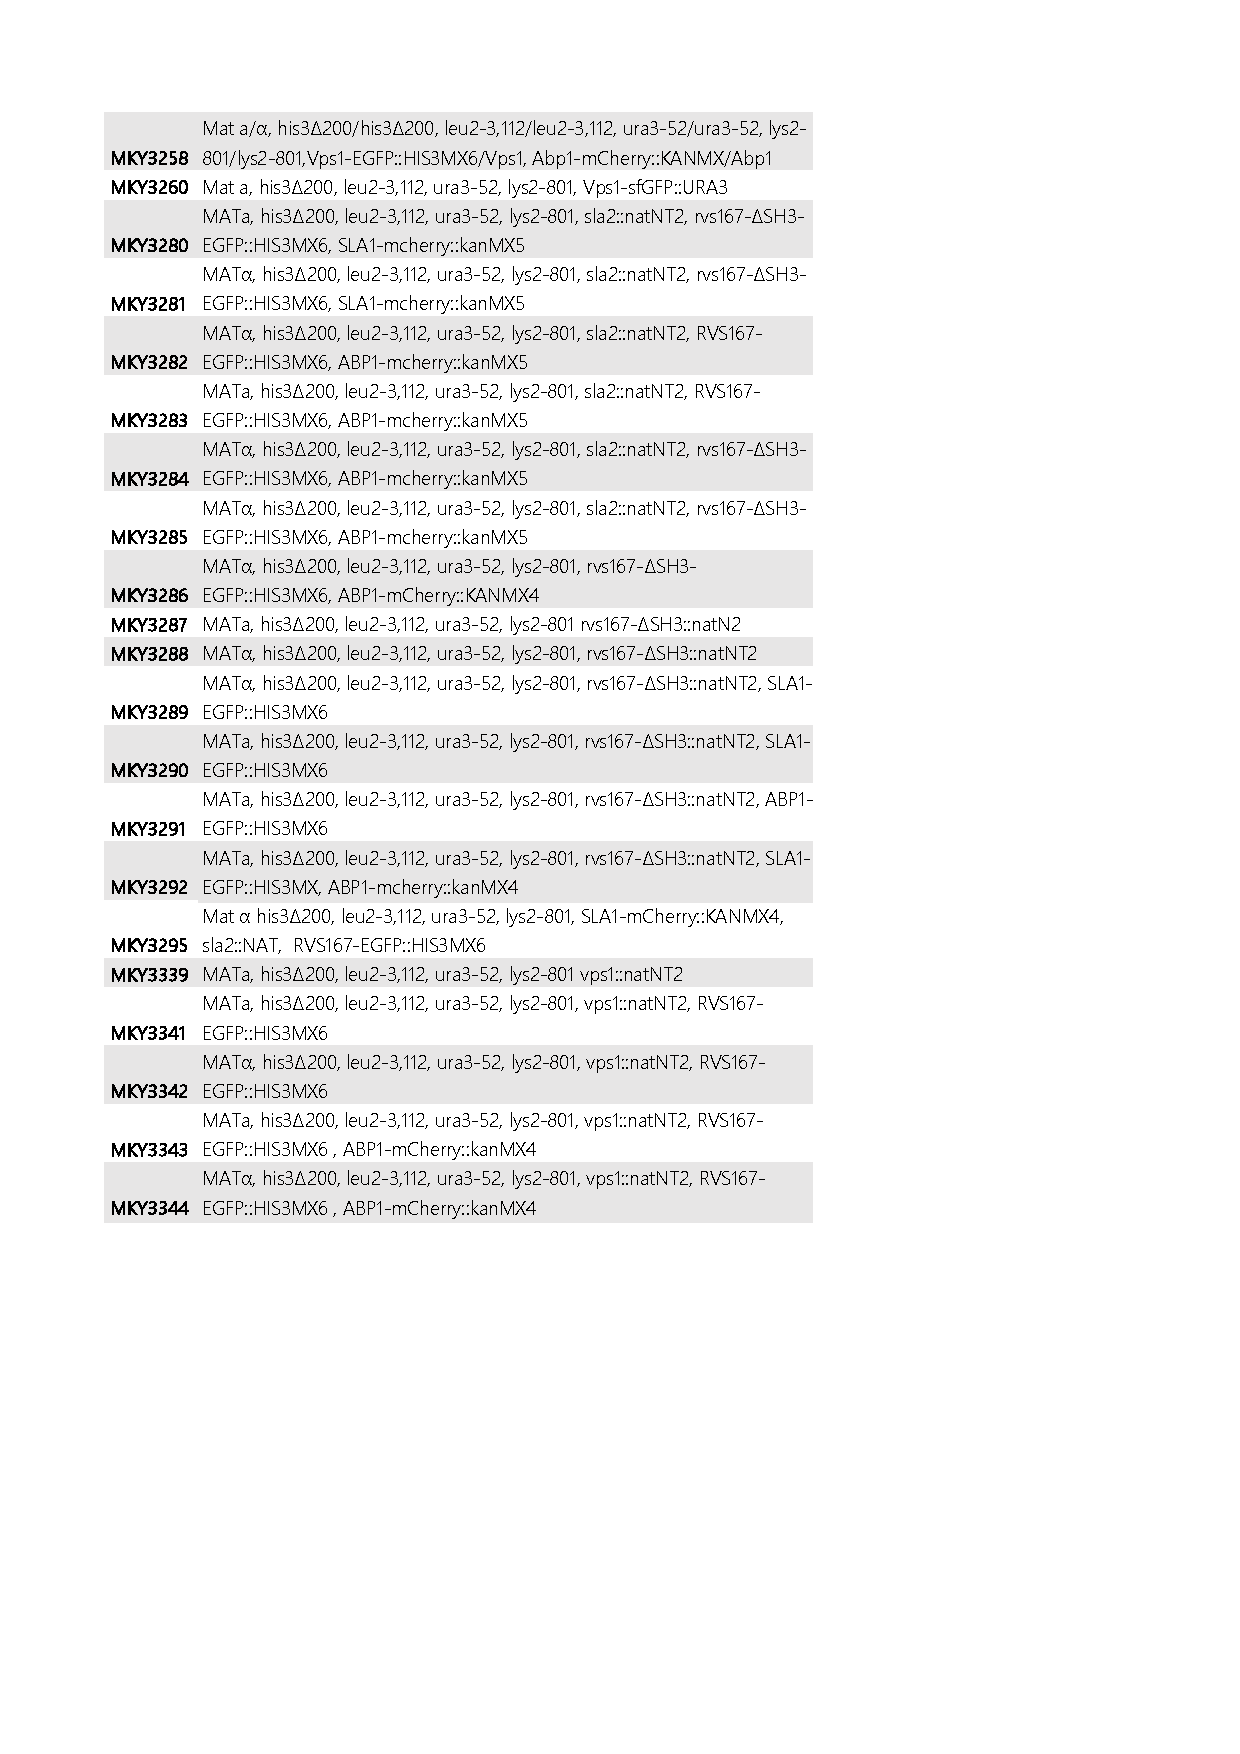
\includegraphics[width=35cm,height=35cm,keepaspectratio, valign=t]{figures/results_final/strains_@2}
\end{table}

\begin{figure}[H]
	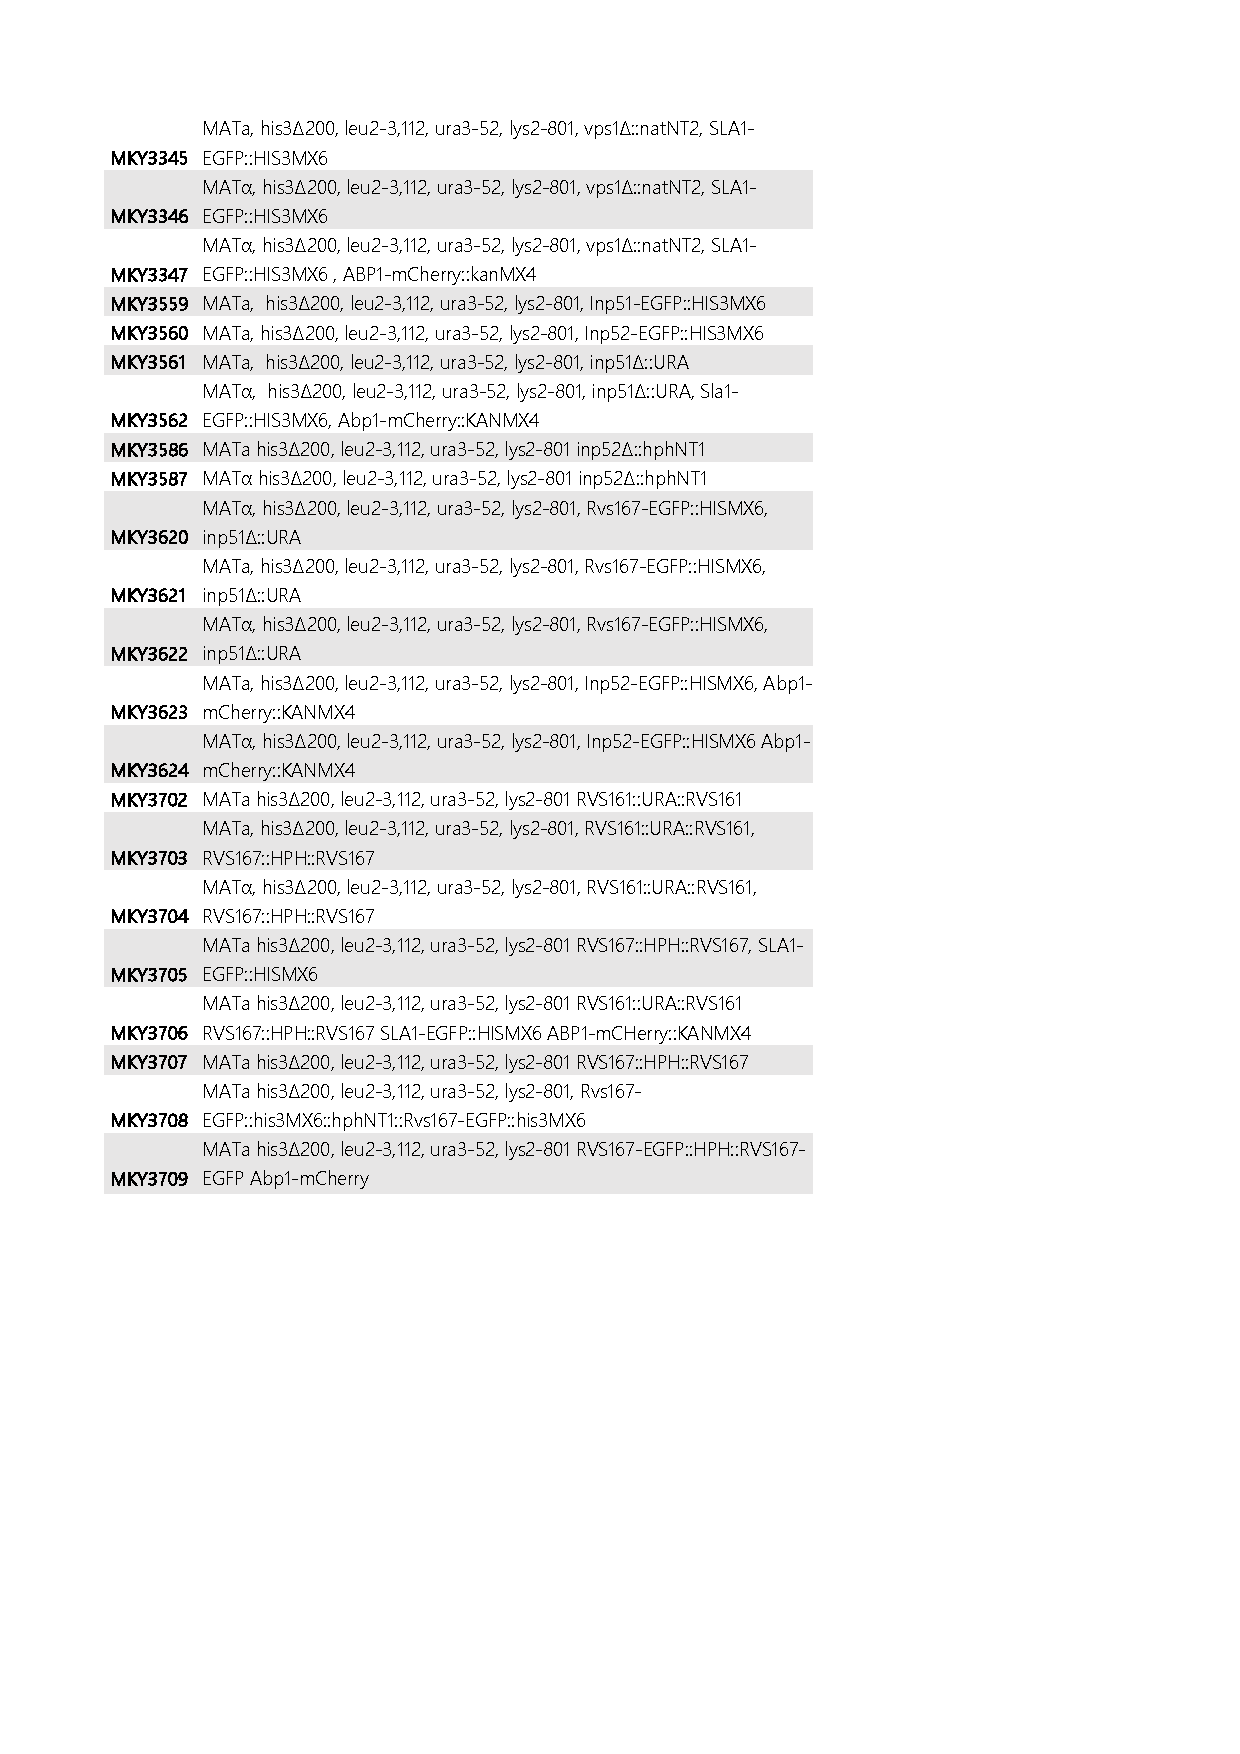
\includegraphics[width=35cm,height=35cm,keepaspectratio, valign=t]{figures/results_final/strains_@3}
\end{figure}

\begin{figure}[H]
	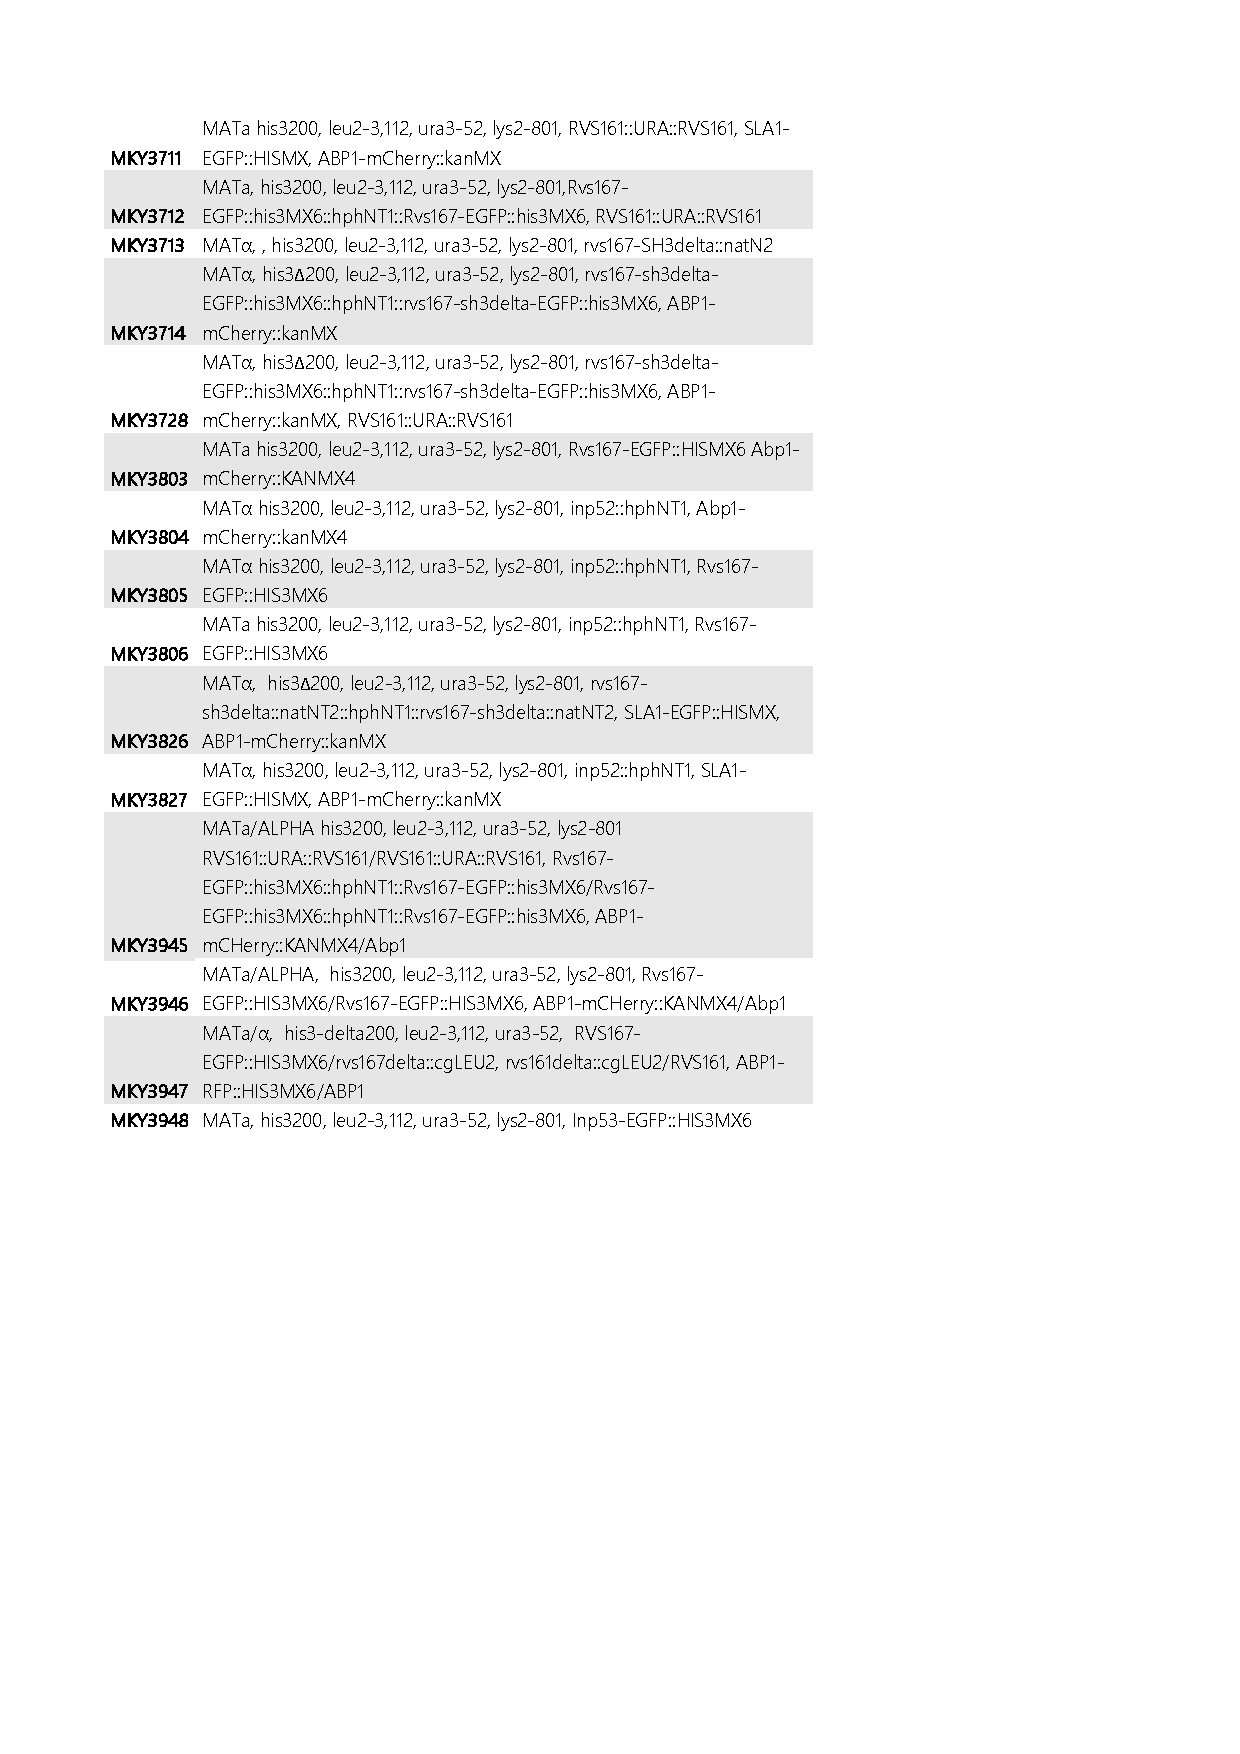
\includegraphics[width=35cm,height=35cm,keepaspectratio, valign=t]{figures/results_final/strains_@4}
\end{figure}

\subsection{Media}
Media was kindly prepared by media kitchens of EMBL and University of Geneva BIochemistry Department, and by Anne-Sophie Riviera of the Kaksonen lab. Plates of all media were made by adding 2\% w/v bacto agar.
All media was autoclaved. Amino acid stocks were filter sterilised and added to the autoclaved media.

\subsubsection{Buffers}

\subsection{Methods}
\subsubsection{Fluorescent tagging yeast with PCR casette insertion}
Tagging or deletion of endogenous genes was done by homologous integration of the product of a Polymerase Chain Reaction using appropriate primers and a plasmid containing a selection cassette and fluorescent tag, or only selection cassette for gene deletions. Primers were designed according to Janke et al, 2004. PCRs used the Velocity Polymerase for fluorescent tagging, and Q5 for gene deletions using the NAT casette. 
All fluorescently tagged genes have a C-terminus tag and are expressed endogenously.
Gene deletions and fluorescent tags are checked by PCR. Vps1del and gene duplications were confirmed by sequencing. 

\subsubsection{Live-cell imaging}
\subparagraph{Sample preparation for live imaging}
			\mbox{}\\
40 μL Concavalin A (ConA) was incubated on a coverslip for 10 minutes. 40 μL Yeast cells incubated overnight at 25C in imaging medium SC-TRP was added to the coverslip after removing the ConA, and incubated for another 10 minutes. Cells were then removed, adhered cells were washed 3x in SC-TRP, and 40 μL SC-TRP was finally added to the coverslip to prevent cells from drying. 

\subparagraph{Sample preparation for live imaging in LatA and Sorbitol treated cells}
\mbox{}\\
Cells went through the same procedure as above till the last washing step. Instead of SC-TRP, 100x diluted LatA, or Sorbitol at a final concentration of 0.2M in SC-TRP was added to the adhered cells. For LatA experiments, cells were incubated in LatA for 10 minutes before imaging. For sorbitol treatments, cells were imaged within 5 minutes of adding sorbitol.

\subparagraph{Epifluorescent imaging for centroid tracking}
			\mbox{}\\
Live-cell imaging was performed as in Picco et al. All images were obtained at room temperature using an Olympus IX81 microscope equipped with a 100×/NA 1.45 PlanApo objective , with an additional 1.6x magnification lens and an EMCCD camera. The GFP channel was imaged using a 470/22 nm band-pass excitation filter and a 520/35 nm band-pass emission filter. mCherry epifluorescence imaging was carried out using a 556/20 nm band-pass excitation filter and a 624/40 band-pass emission filter. GFP was excited using a 488 nm solid state laser and mCherry was excited using a 561 nm solid state laser. Hardware was controlled using Metamorph software. For single-channel images, 80-120ms was used as exposure time. All dual-channel images were acquired using 250ms exposure time. Simultaneous dual-color images were obtained using a dichroic mirror, with TetraSpeck beads used to correct for chromatic abberation.

\subparagraph{Epifluorescent imaging for molecule number quantification}
			\mbox{}\\
Images were acquired as in Picco et al. Z-stacks of cells containing the GFP-tagged protein of interest, incubated along with cells containing Nuf2-GFP, were acquired using 400ms exposure using a mercury vapour lamp, on a CCD camera. Z stacks were spaced at 200nm. 

\subparagraph{TIRF imaging}
			\mbox{}\\
TIRF microscopy was performed under similar conditions on an Olympus IX83 microscope. GFP was excited using a 488 nm solid state laser and mCherry was excited using a 561 nm solid state laser. Lasers, and shutters were controlled by Visitron Systems VS-Laser Control. VisiView software controlled the image acquisition and hardware-software feedback.
Images were processed using ImageJ, quantification was done on R.

\subsubsection{Live-cell Image analysis}
Images were processed for background noise using a rolling ball radius of 90 pixels. Particle detection, and tracking was performed for a particle size of 6 pixels, using scripts that combine background subtraction with Particle Tracker and Detector, that can be found on ImageJ (http://imagej.nih.gov). Further analysis for centroid averaging, alignments between dual-color images and single channel images, for alignment to the reference Abp1 were done using scripts written in Matlab (Mathworks) and R (www.r-project.org), written originally by Andrea Picco, and modified by me. Details of analysis can be found at Picco et al. All movement and intensity plots from centroid tracking show the average centroid with 95\% confidence interval. All molecule number quantifications report either the median or maximum number of molecules with standard error of mean. Maximum number is preferred over median in cases when the rate of change of fluorescent intensity of two populations being compared are not similar, and the lifetime of the protein populations being compared are not similar. The median in this case underreports the differences in protein accumulation. 


\subsubsection{CLEM}
Samples were prepared for CLEM as described in Wanda et al. Briefly, cells expressing Rvs167-GFP and Abp1-mCherry, and BAR-GFP and Abp1-mCherry cells were grown overnight in YPD, at 24C. They were then diluted to an OD600 of 0.2, and grown to OD600 between 0.8 and 1.2. These cells were then concentrated to a filter paper using a vacuum pump, and high-pressure frozen. Samples were freeze substituted in Lowycryl HM20 using the Kukulski freeze substitution protocol using an automated robot. 
\vspace{2mm}
Samples in resin were sliced to 300nm sections using a diamond knife, and loaded to carbon-coated copper grids. TetraSpec beads were incubated on the slices and these slices were imaged using epifluorescence microscopy in GFP and RFP channels for GFP and m-Cherry, and Cyan channel for separating the signal from the Tetraspec beads, that would later be used as fiducials to correlate these fluorescent images with electron tomograms. 
\vspace{2mm}
Gold fiducials were incubated on the grids, and lead citrate was added to stain the membrane. Low magnification tilts were acquired at 3 degree increments. High magnification tilts were perfomed at 1 degree increments from -60 to 60 degrees. Tomograms were reconstructed using IMOD. Invagination lengths were measured at the longest axis of the invagination, using IMOD.



 
\chapter*{Bibliography} % Main chapter title
\addcontentsline{toc}{chapter}{Bibliography}
\pagestyle{plain}

\pm

\begin{figure}[H]
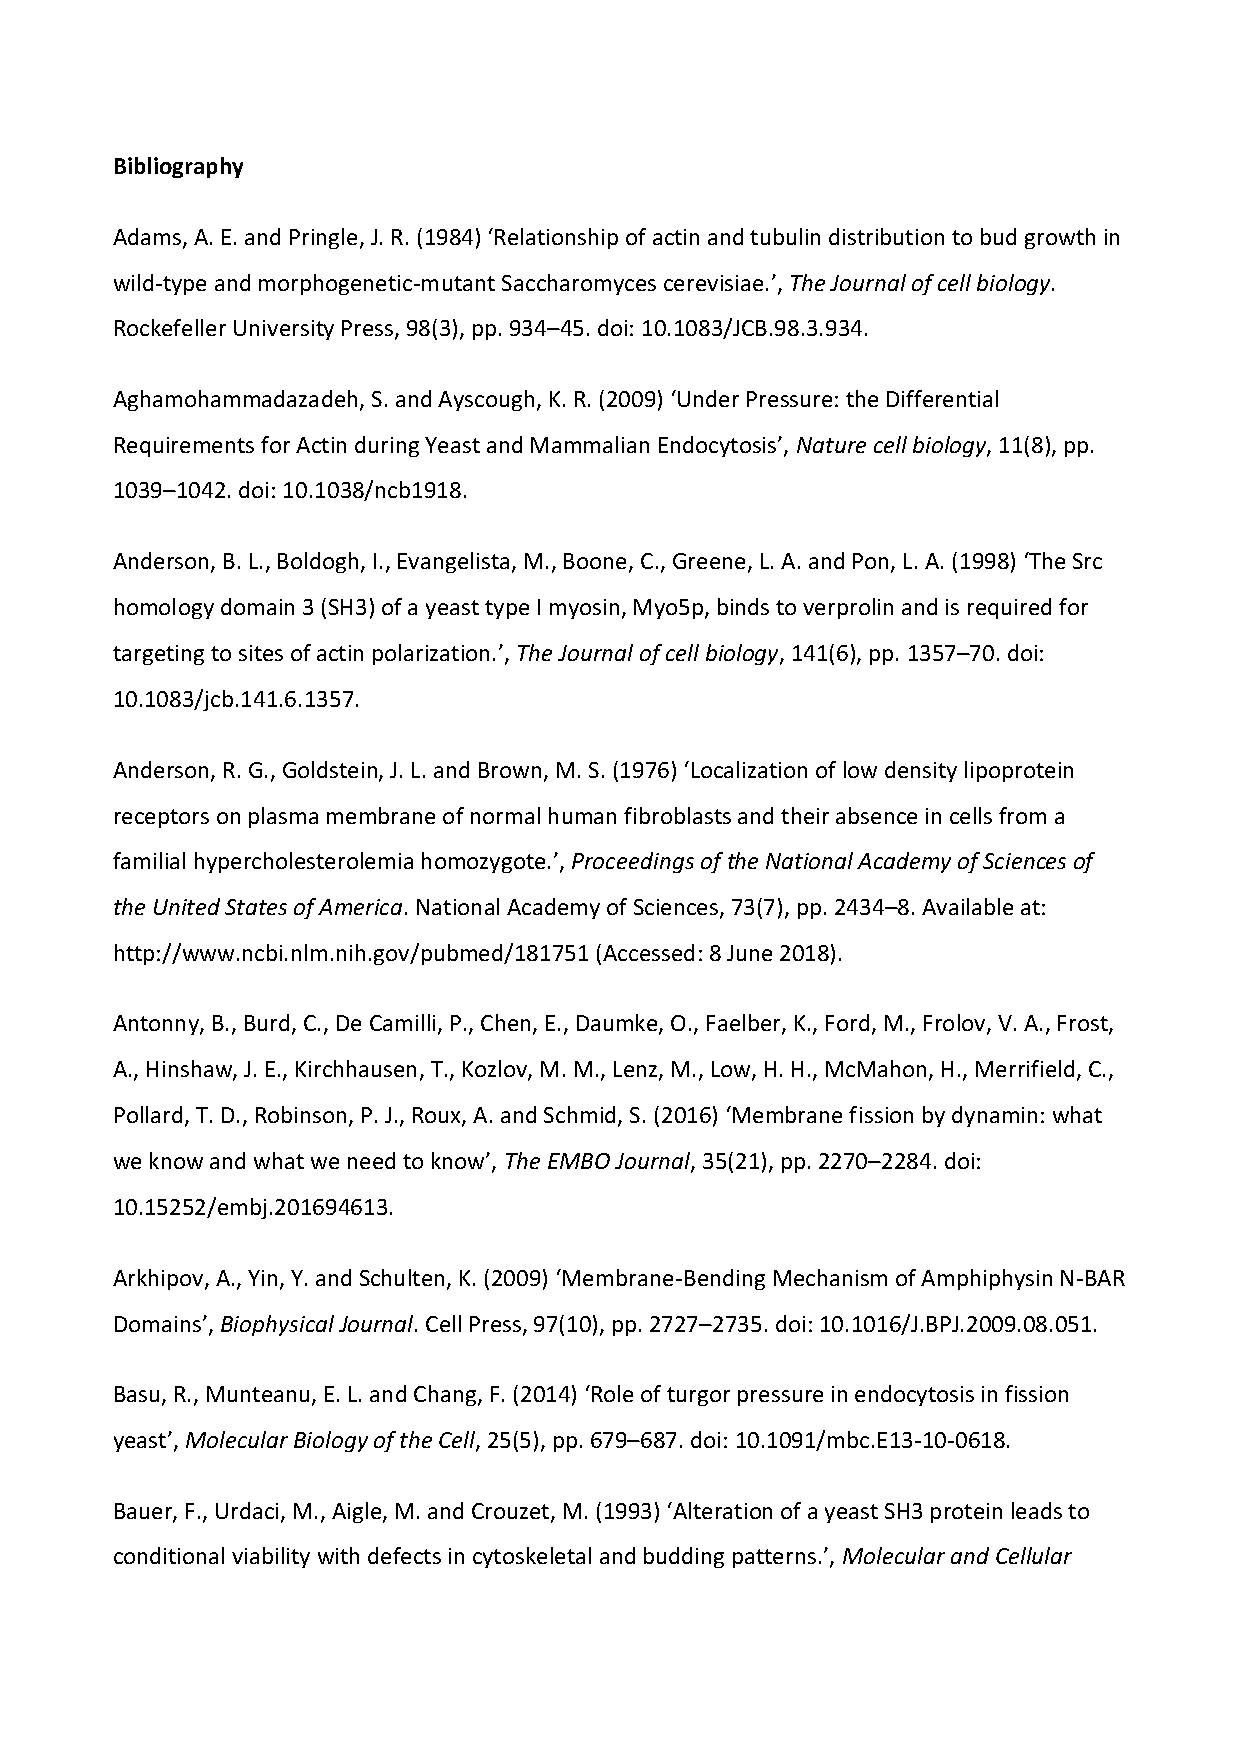
\includepdf[pages={1}]{merge_20180817.pdf}
\end{figure}

%\includepdf[pages=-]{myfile.pdf}
%\includepdf[pages={1}]{myfile.pdf} 

%----------------------------------------------------------------------------------------
%	THESIS CONTENT - APPENDICES
%----------------------------------------------------------------------------------------

\appendix % Cue to tell LaTeX that the following "chapters" are Appendices

% Include the appendices of the thesis as separate files from the Appendices folder
% Uncomment the lines as you write the Appendices

\chapter*{Appendix} % Main chapter title
\addcontentsline{toc}{chapter}{Appendix}

\begin{figure}[H]
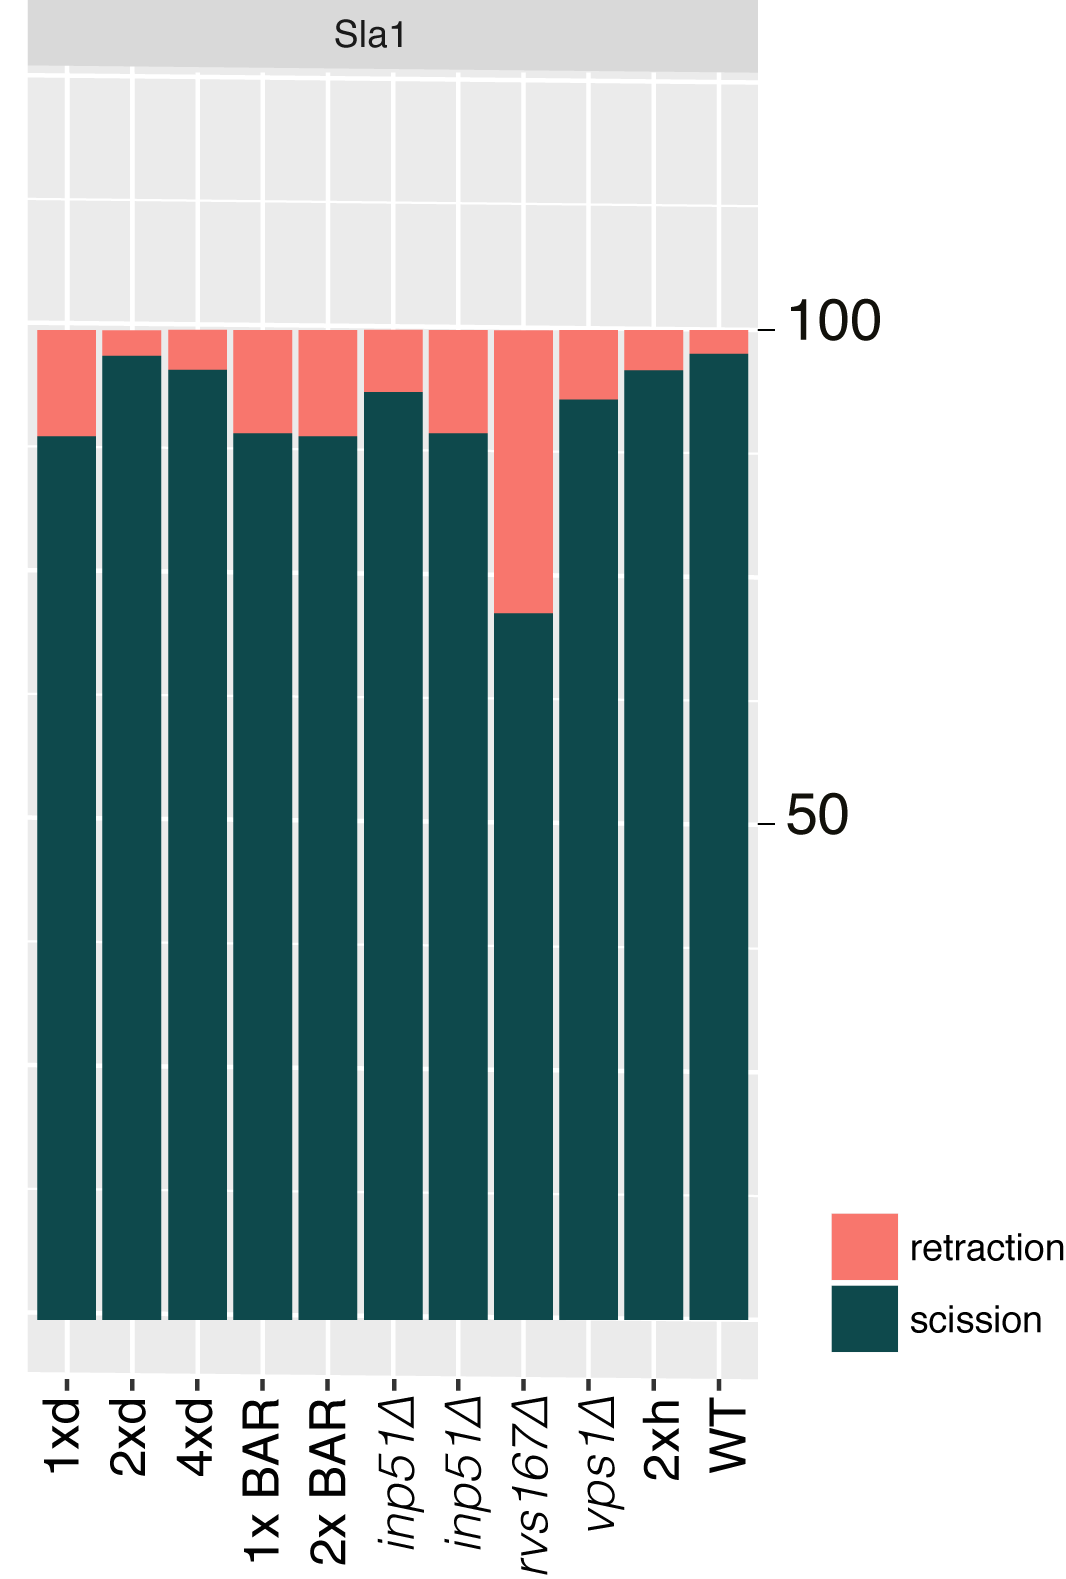
\includegraphics[scale=1.5]{figures/appendix/retraction_rates_all}
\caption{Sla1-GFP retraction rates}
\end{figure}


\begin{figure}[H]
	\includegraphics[scale=1.5]{figures/appendix/table2l}
	caption{Cytoplasmic intensities}
\end{figure}
\include{Appendices/AppendixB}
%\include{Appendices/AppendixC}

%----------------------------------------------------------------------------------------
%	BIBLIOGRAPHY
%----------------------------------------------------------------------------------------
%\appto{\bibsetup}{\raggedright}
%renewcommand*{\bib}{\small}
%\setstretch{0.9}
%\setlength\bibitemsep{6pt}
%\begingroup \sloppy

%\bibliographystyle{plainnat}
%\bibliography{library.bib}

%\printbibliography[heading=bibintoc]
 
%\par \endgroup

%\addcontentsline{file}{section_unit}{Bibliography}
%\chapter{Bibliography}
%\addcontentsline{toc}{chapter}{Bibliography}
%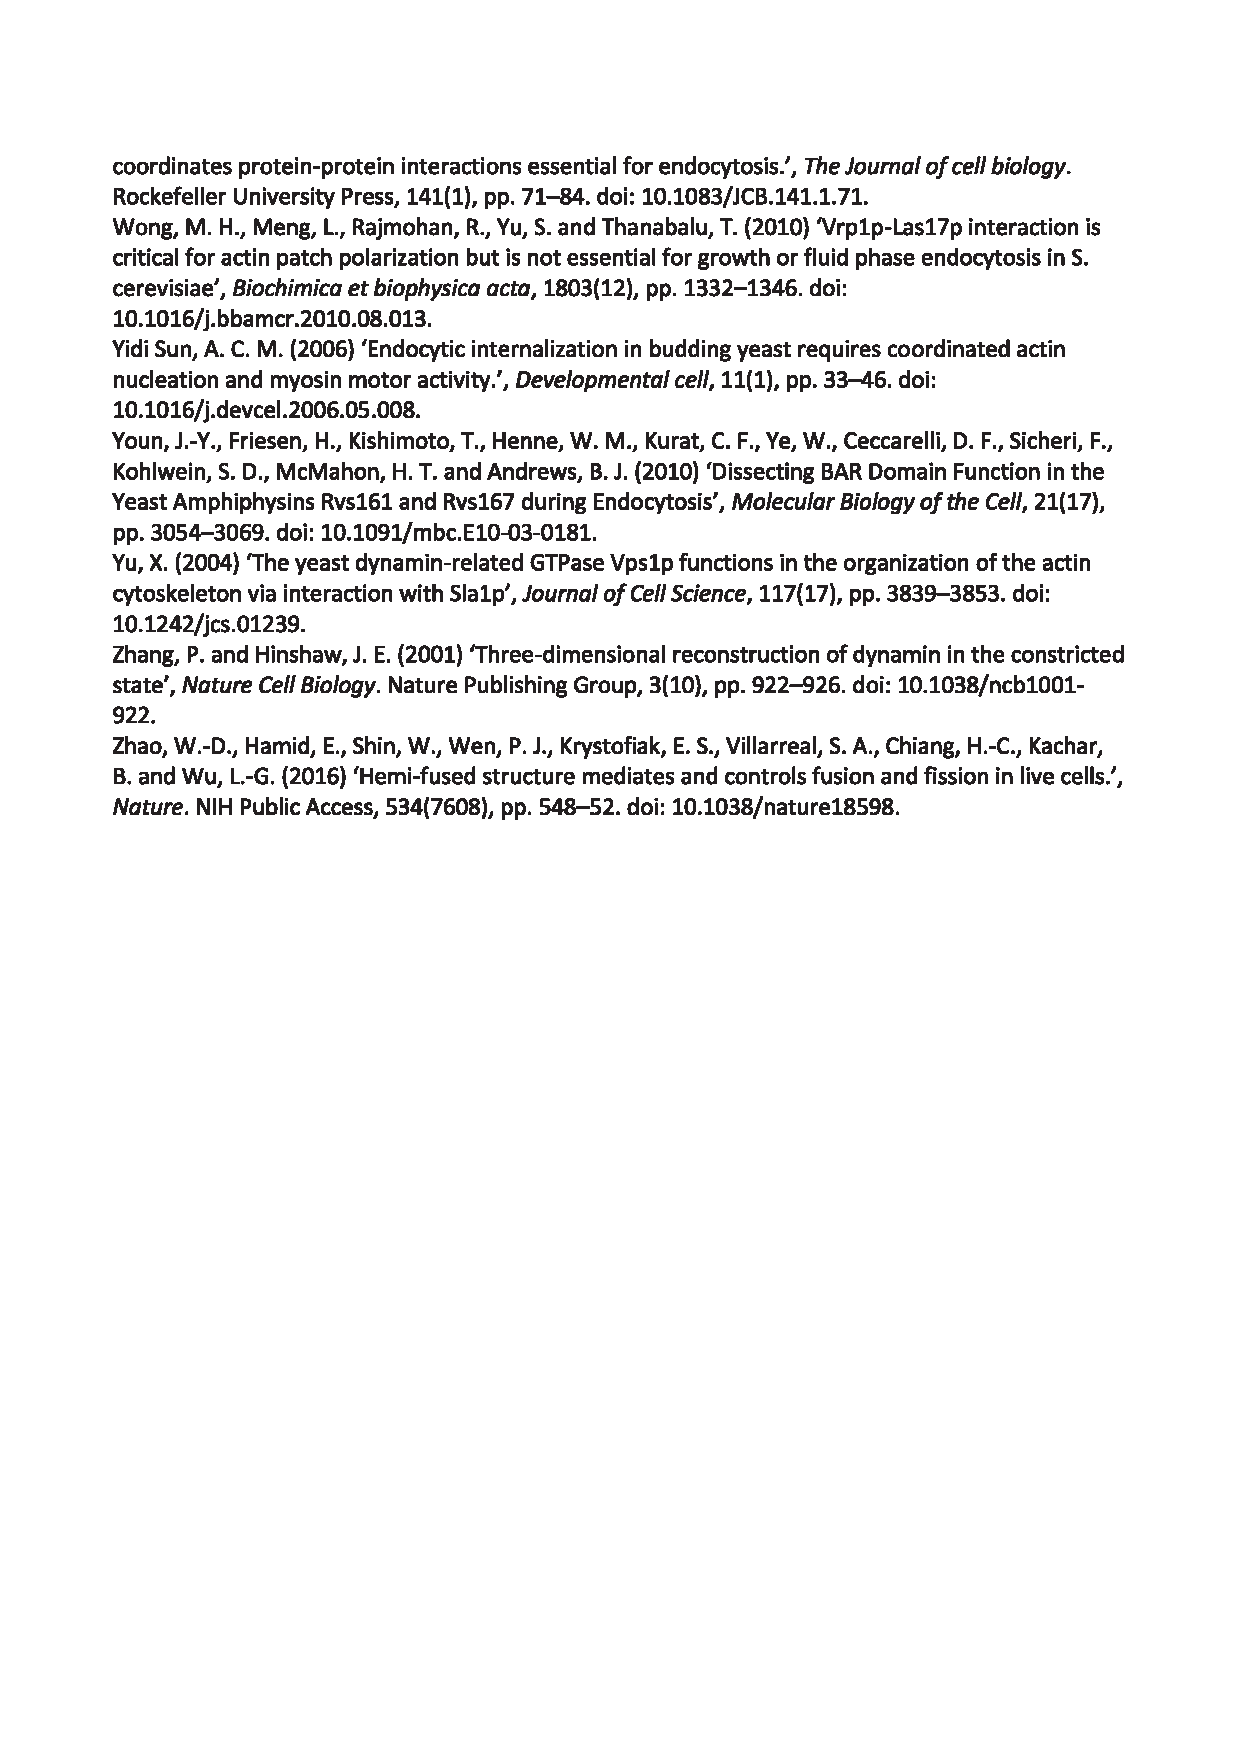
\includegraphics{parts/bib_end}
%----------------------------------------------------------------------------------------

\end{document}  
